%\documentclass[12pt,a4paper]{report}
\documentclass[12pt,a4paper,oneside,onecolumn,openright]{book}
% set the document language
\usepackage[italian]{babel}
% set the encoding used by your editor here (default is utf8)
\usepackage[utf8]{inputenc}
\usepackage[T1]{fontenc}

% math packages
\usepackage{amsmath}
\usepackage{amssymb}
\usepackage{lmodern}
\usepackage{varwidth}
\usepackage{xcolor}
\usepackage[makeroom]{cancel}
% page margins settings
\usepackage[inner=1.5cm,outer=1.5cm,top=1.5cm,bottom=1.5cm]{geometry}
%\usepackage{indentfirst}

% other packages
\usepackage{array}
\usepackage{enumitem}
\usepackage{subfigure}
\usepackage{graphicx}
\usepackage{verbatim}
\usepackage{listings}
\usepackage{url}
\usepackage[hidelinks]{hyperref}
\usepackage[export]{adjustbox}
\usepackage{latexsym}
\usepackage{tabularx}
\usepackage{ragged2e}
\usepackage{mathtools}
\DeclarePairedDelimiter\floor{\lfloor}{\rfloor}
\DeclarePairedDelimiter\ceil{\lceil}{\rceil}
% \usepackage{Mathematics}
% custom colors
\usepackage{color}
\usepackage{wrapfig}
\usepackage{gensymb}
\usepackage{caption}
\usepackage{tikz}
\usetikzlibrary{arrows.meta, positioning}
\usepackage{forest}
\usepackage{tikz-qtree}

\newcommand\myeq{\stackrel{\mathclap{\tiny\mbox{def}}}{=}}

\usepackage[many]{tcolorbox}
\newtcolorbox{boxA}{
    % fontupper = \bf,
    boxrule = 1.5pt,
    colframe = black % frame color
}

\usetikzlibrary{shadows}
\definecolor{light-gray}{gray}{0.96}
\definecolor{cyan}{RGB}{230,230,255}
\definecolor{dkgreen}{rgb}{0,0.6,0}
\definecolor{gray}{rgb}{0.5,0.5,0.5}
\definecolor{mauve}{rgb}{0.58,0,0.82}
\definecolor{iceberg}{rgb}{0.44, 0.65, 0.82}
% \definecolor{blue}{RGB}{44, 44, 210}

\hypersetup{
colorlinks=true,
linkcolor=black,
% filecolor=blue,
urlcolor=blue,
% pdftitle={Overleaf Example},
}

\urlstyle{same}
\graphicspath{ {./images/} }

% environment for bash code
\lstset{ %
  language=bash,                % the language of the code
  basicstyle=\footnotesize,           % the size of the fonts that are used for the code
  numbers=left,                   % where to put the line-numbers
  numberstyle=\footnotesize,          % the size of the fonts that are used for the line-numbers
  stepnumber=1,                   % the step between two line-numbers. If it's 1, each line 
                                  % will be numbered
  numbersep=5pt,                  % how far the line-numbers are from the code
  backgroundcolor=\color{white},      % choose the background color. You must add \usepackage{color}
  showspaces=false,               % show spaces adding particular underscores
  showstringspaces=false,         % underline spaces within strings
  showtabs=false,                 % show tabs within strings adding particular underscores
%  frame=single,                   % adds a frame around the code
  rulecolor=\color{black},        % if not set, the frame-color may be changed on line-breaks within not-black text (e.g. commens (green here))
  tabsize=2,                      % sets default tabsize to 2 spaces
  captionpos=b,                   % sets the caption-position to bottom
  breaklines=true,                % sets automatic line breaking
  breakatwhitespace=false,        % sets if automatic breaks should only happen at whitespace
  title=\lstname,                   % show the filename of files included with \lstinputlisting;
                                  % also try caption instead of title
  numberstyle=\tiny\color{gray},        % line number style
  keywordstyle=\textbf,          % keyword style
  commentstyle=\color{dkgreen},       % comment style
%  stringstyle=\color{mauve},         % string literal style
  escapeinside={\%*}{*)},            % if you want to add a comment within your code
  morekeywords={*,...,insert,-}               % if you want to add more keywords to the setù
}

% environment for python code
\lstset{
	language=Python,
	breaklines=true,
	breakatwhitespace=true ,
	backgroundcolor=\color{light-gray}
}

\newcommand{\grayScale}{0.95} % Can change the gray level here
\definecolor{codeBackground}{rgb}{\grayScale ,\grayScale ,\grayScale}
\definecolor{forestGreen}{rgb}{0.13,0.55,0.13}

\lstset{
    language=C,
    backgroundcolor=\color{codeBackground},
    tabsize=4,
    showstringspaces=false,
    showtabs=false,
    showspaces=false,
    basicstyle=\ttfamily,
    identifierstyle=\ttfamily,
    keywordstyle=\color{blue},
    stringstyle=\color{red},
    commentstyle=\color{gray},
    numberstyle=\color{magenta},
    morecomment=[l][\color{forestGreen}]{\#},
    % escapechar={|}, 
}
% appendices package
%\usepackage{appendix}
% set Appendix name used in the toc
%\renewcommand{\appendixtocname}{Appendice}

% interline
\linespread{1.5}
% set numbers for subsections and show them in the toc
\setcounter{tocdepth}{3} 
\setcounter{secnumdepth}{3}

% layout package, style and settings
\usepackage{fancyhdr}
\pagestyle{fancy}

\fancypagestyle{mainmatter}{%		
		\fancyhf{} 
		\fancyhead{}
		\fancyhead[LE,RO]{\thepage}
		\fancyhead[LO]{\footnotesize{\leftmark}}
		\fancyhead[RE]{\footnotesize{\rightmark}}
		\fancyfoot{}
		\addtolength{\headwidth}{\marginparsep}
		\addtolength{\headheight}{2.5pt}
		\renewcommand{\headrulewidth}{0.3pt}
		\renewcommand{\footrulewidth}{0.0pt}
		}
\fancypagestyle{frontmatter}{%
		\fancyhf{} 
		\fancyhead[LE]{\footnotesize{\MakeUppercase{\thepage}}}
		\fancyhead[RO]{\footnotesize{\MakeUppercase{\thepage}}}
		\fancyhead[RE,LO]{}
		\fancyfoot{}
		\addtolength{\headwidth}{\marginparsep}
		\addtolength{\headheight}{2.5pt}
		\renewcommand{\headrulewidth}{0.0pt}
		\renewcommand{\footrulewidth}{0.0pt}
		}
		
		
\usepackage{fancyhdr}
\pagestyle{fancy}
		\fancyhf{} 
		\fancyhead{}
		\fancyhead[LE,RO]{\thepage} 
		\fancyhead[LO]{\footnotesize{\leftmark}}
		\fancyhead[RE]{\footnotesize{\rightmark}}
		\fancyfoot{}
		\addtolength{\headwidth}{\marginparsep}
		\addtolength{\headheight}{2.5pt}
		\renewcommand{\headrulewidth}{0.3pt}
		\renewcommand{\footrulewidth}{0.0pt}

% empty pages have no numbers
\makeatletter
\def\cleardoublepage{\clearpage\if@twoside \ifodd\c@page\else
\hbox{}
  %Potresti voler togliere il commento dalla linea seguente
  %Questa pagina � stata lasciata intenzionalmente vuota.
\thispagestyle{empty}
\newpage
\if@twocolumn\hbox{}\newpage\fi\fi\fi}
\makeatother
%????
%\textwidth=450pt\oddsidemargin=0pt

%\makeatletter 
%  \DeclareRobustCommand*\textsubscript[1]{% 
%    \@textsubscript{\selectfont#1}} 
%  \newcommand{\@textsubscript}[1]{% 
%    {\m@th\ensuremath{_{\mbox{\fontsize\sf@size\z@#1}}}}} 
\makeatother 

\begin{document}
\begin{titlepage}
\begin{center}
{
    \large
    \textbf{Università  degli studi di Modena e Reggio Emilia} \\
   	\textbf{Dipartimento di Ingegneria Enzo Ferrari} \\
    \vspace{\stretch{0.5}}
    \hspace*{0cm} \hrulefill \hspace*{0cm} \\
    \vspace{\stretch{0.5}}    
	  \vspace{\stretch{12}}
  
  
 		\huge{\bf Crittografia Applicata }}\\
		\vspace{3mm}
		
		\vspace{\stretch{6}}
		\end{center}
		
\vspace{40mm}
\par
\noindent
\vspace{20mm}
\begin{center}
\hspace*{0cm} \hrulefill \hspace*{0cm} \\
{\large{\bf 
Anno Accademico 2023/24}}
\end{center}

\end{titlepage}

\pagestyle{frontmatter}
\frontmatter

% PAGINA VUOTA
%\clearpage\null\thispagestyle{empty}\clearpage
\setcounter{tocdepth}{2}
\tableofcontents

\setlength{\parindent}{12pt}
\setlength{\parskip}{1ex plus 0.5ex minus 0.2ex}
\mainmatter
\pagestyle{mainmatter}

\chapter{Introduction}

\section{Structure and Content}
\begin{itemize}

    \item \textbf{Module 1}: 
    \begin{enumerate}
        \item \textbf{\textit{intra-vehicles communications}}: nodes, sensors, ECU
        \item \textbf{\textit{signal busses}}: CAN, LIN, FlexRay, MOST, Ethernet [ T1/T1S]
        \item \textbf{\textit{car domain and OS}}
    \end{enumerate}
    
    \item \textbf{Module 2}:
    \begin{enumerate}
        \item \textbf{\textit{inter-vehicles communications}}: \textit{V2V} and \textit{V2X} (car is a node)
        \item \textbf{\textit{wireless technologies}}: Bluetooth, LoRa, C-V2X, IEE 802.11p (bd)
        \item application, messages, broadcast, GPS
    \end{enumerate}

\end{itemize}
Different \textbf{domain} or \textbf{application} needs different \textit{communications protocols}, is important to understand how each nodes in domain communicate each other (inside the car).

\newpage
\section{Intra-Vehicles}
From the 80's, where the car's control unit are isolated an there was a dedicated wires connect sensors and actuators with less electronic than now, until the reach the greates goal of evolution in the automotive sector: autonomous drive. The complexity of the number of connection from each ECU's to the other, also the number of ECU's for each car, is growing. While the number of signal increase in a liner way, the connection between ECU's is growing with a quadratic complexity $O(n^2)$.

If we examine the evolutions of the ECUs number inside an ``Audi A6'' we can observe that in 1997 it has 5 ECUs and in the 2007 it has 50 ECUs, instead the ``Tesla M3'' in the 2017 has 70 ECUs. The quadratic increase of ECUs number, however has reach a cap for two main reason: the cost and the space inside the car. Traditionally one ECUs is responsible of one task, but nowadays it could be two type of trends:
\begin{enumerate}[nosep]
    \item \textit{distributed of function across ECUs}
    \item \textit{integration of multiple function in one ECU}
\end{enumerate}

\section{Architectures}

\begin{figure}[h]
    \centering
    \begin{minipage}[t]{0.45\textwidth}
        \centering
        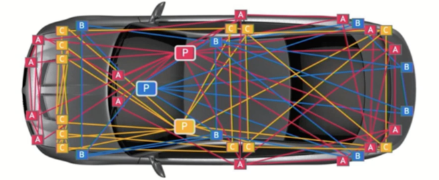
\includegraphics[width=\textwidth]{img/domain_architecture}
        \caption{\textit{Domain Architecture}}
        
        \begin{flushleft}
            \begin{enumerate}[nosep]
                \item central domain controller (\textbf{P}) or high performance computer
                \item ability to handle more complex functions
                \item cost optimization
                \item cable harness is rigid and expensive
            \end{enumerate}
        \end{flushleft}

    \end{minipage}
    \begin{minipage}[t]{0.45\textwidth}
        \centering
        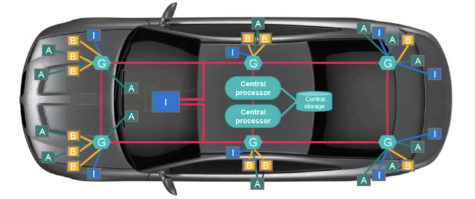
\includegraphics[width=\textwidth]{img/zonal_architecture}
        \caption{\textit{Zonal Architecture}}
        
        \begin{flushleft}
            \begin{enumerate}[nosep]
                \item local ethernet per zone (\textbf{G})
                \item ultra high-speed secured backbone between zone
                \item centralized software
                \item central computer storage
            \end{enumerate}
        \end{flushleft}
        
    \end{minipage}
\end{figure}
\chapter{Crittografia Simmetrica}

\begin{figure}[h]
    \centering
    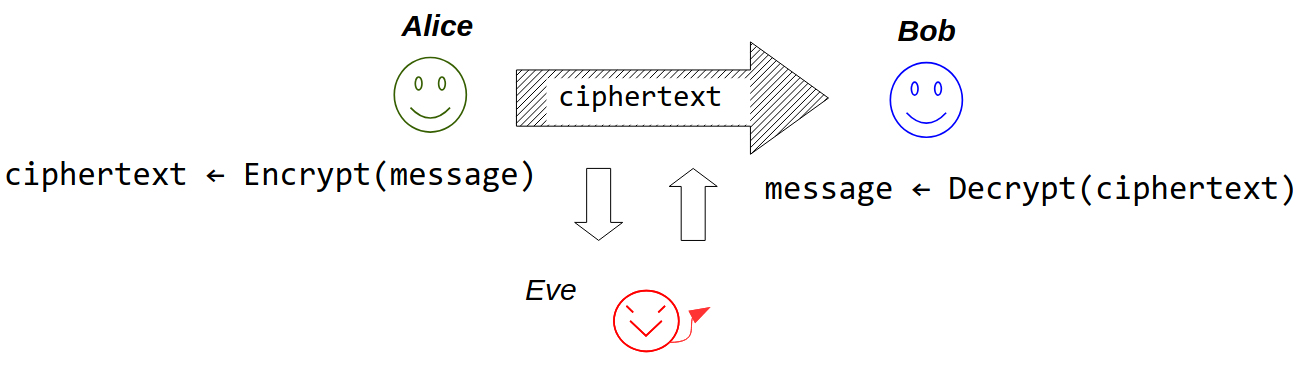
\includegraphics[width=\textwidth]{img/crypto_symm_1.png}
\end{figure}

Le garanzie di sicurezze che si cercano di mantenere sono:
\begin{itemize}[nosep]
    \item \textbf{confidenzialità}: Eve non può accedere a nessuna della informazioni sul messaggio.
    \item \textbf{autenticazione}: Bob può verificare se il messaggio non è stato inviato da Alice, viene anche chiamata \textbf{\textit{data orgin authenticity}} nel contesto della comunicazioni e implica anche la protezione contro modifiche illegittime (\textbf{integrità}).
\end{itemize}

\begin{flushleft}
    La sicurezza non esiste in natura è quindi necessario idearla e modellarla, questa prima parte prende il nome di \textit{Definitional Activity}. È comunque importante ricordare che le \textbf{definizioni} possono essere \textbf{errate} principalmente per errori nella modellazione o nello sviluppo software, ma anche perché non si è stato in grado di modellare quello che era invece richiesto. Un altro errore che si può essere portati a fare è quello di utilizzare in maniera errata certe definizioni ad esempio al di fuori del contesto per cui era stata definita. \newline
    \textbf{\textit{Definitional Activity}}: permette di descrivere che cosa l'avversario può \textbf{fare} e cosa può \textbf{vedere}. Esistono molteplici modi per definire la sicurezza in maniera più formale, uno tra questi è la \textbf{\textit{simulation-based security}} dove viene definita una funzione ideale che soddisfa la definizione di security e poi dimostrare che la funzione costruita si comporti come quella ideale.
\end{flushleft}

\begin{figure}[h]
    \centering
    \begin{large}
        \textbf{\textit{First Adversary Model}} \\
    \end{large}
    Quindi modelliamo e identifichiamo le casistiche e tipologie di un attaccante. \\

    \begin{minipage}[t]{0.50\textwidth}
        \centering
        \begin{boxA}
            \textcolor{red}{\textbf{\textit{Attack Model: Passive Eavesdropper (EAV)}}} \\
            Ha capacità di lettura dei soli \textit{ciphertext} e non è capace di \textbf{scegliere nulla}
        \end{boxA}
    \end{minipage}
    \begin{minipage}[t]{0.45\textwidth}
        \centering
        \begin{boxA}
            \textcolor{red}{\textbf{\textit{Security Goal: Indistinguishably}}} \\
            L'avversario non può distinguere il \textit{ciphertext} da sequenza di caratteri random.
        \end{boxA}
    \end{minipage}
\end{figure}

\begin{flushleft}
    Modellando in questo modo il nostro avversario è possibile osservare che non viene descritto nulla sul nascondere la lunghezza del \textit{plaintext}, infatti per questa prima modellazione l'avversario può vedere la lunghezza del \textit{plaintext}. \\
    \textbf{Nota}: la crittografia non ha come obiettivo quello di nascondere la lunghezza del testo in chiaro, nel caso in cui questa informazione fosse confidenziale, è necessario proteggerla a livello applicativo.
\end{flushleft}

\begin{flushleft}
    Le capacità di un avversario vengono espresse e descritte tramite degli algoritmi chiamati \textbf{esperimenti}, che vengono eseguiti da un'entità chiamata \textbf{\textit{challenger}} (che per semplicità andiamo ad identificare nell'attore onesto). \\
    Come prima andiamo ad analizzare \textbf{\textit{IND-EAV}}, il \textit{challenger} va a scegliere un messaggio \textbf{m} che viene scelto con la stessa probabilità tra:
    \begin{itemize}[nosep]
        \item dati random: $m \leftarrow \{0, 1\}^n$
        \item un messaggio generato attraverso la cifrazione $m = \text{Encryption}(p)$, dove \textbf{p} può essere scelto nello stesso modo di prima $p \leftarrow \{0, 1\}^n$
    \end{itemize}
    All'avversario viene fornito \textbf{m} e deve scegliere se è un messaggio randomico o se è l'output dell'\textit{encryption}, l'avversario vince l'esperimento se la sua decisione è corretta.
\end{flushleft}

\begin{flushleft}
    \textcolor{red}{\textbf{\textit{IND-EAV: Perfect \& Computational Indistinguishably}}} \\
    Andremo a discutere due tipologie di sicurezza:
    \begin{enumerate}[nosep]
        \item \textbf{\textit{perfect}}: la probabilità dell'avversario di vincere l'esperimento è del \textbf{50\%}, viene anche chiamata \textbf{\textit{Unconditional Security}} o \textbf{\textit{Informatition Theoretic Security}}.
        \item \textbf{\textit{computational}}: la probabilità dell'avversario di vincere l'esperimento è \textbf{50\%} più una \textbf{quantità trascurabile}.
    \end{enumerate}
    Qualunque tipologia di schema \textbf{praticabile} garantisce \textbf{sicurezza computazionale}, e se capace di essere sicuro contro un'\textbf{esperimento IND-EAV} viene detto \textbf{\textit{IND-EAV secure}}.
\end{flushleft}

\section{Sicurezza Incondizionata \& One-Time Pad}
\textcolor{red}{\textbf{XOR}}: gli schemi di crittografia moderni sono progettati per \textbf{dati binari}. L'operazione base per la crittografia simmetrica è lo \textbf{XOR}.

\begin{center}
    \begin{minipage}[c]{0.3\textwidth}
        \centering
        $c = m \oplus k$
    \end{minipage}
    \begin{minipage}[c]{0.3\textwidth}
        \centering
        \begin{tabular}{|c|c|c|}
            \hline
            \textbf{m} & \textbf{k} & \textbf{c} \\ \hline
            0 & 0 & 0 \\ \hline
            0 & 1 & 1 \\ \hline
            1 & 0 & 1 \\ \hline
            1 & 1 & 0 \\ \hline
        \end{tabular}
    \end{minipage}
    \begin{minipage}[c]{0.3\textwidth}
        \centering
        \textbf{Nota}: lo \textbf{XOR} può essere anche modellato come la somma bit per bit modulo 2: $c_i = (m_i \oplus k_i) \; \text{mod} \; 2$
    \end{minipage}
\end{center}

\begin{flushleft}
    Lo XOR viene scelto perché dato un certo \textbf{m}, se \textbf{k} viene scelta in maniera randomica la probabilità di \textbf{c} di essere \textbf{0} o \textbf{1} è \textbf{p = 0.5}. \\
    In questo modo sapere \textbf{c} non da informazioni su \textbf{m} e quindi \textbf{c} è indistinguibile da una successioni di bit random: $\{0, 1\}^n$
\end{flushleft}

\begin{flushleft}
    \textcolor{red}{\textbf{\textit{One-Time Pad - Vernam's Cipher}}}: è un algoritmo di crittografia che esegue un XOR bit a bit tra il testo in chiaro e la chiave, le due lunghezze devono essere uguali e la chiave devere essere random. $c_i = m_i \oplus k_i \; \forall i \in \{0, ..., n\}$ dove $n$ è la lunghezza del testo in chiaro. \\
    Per la decifrazione bisogna utilizzare la stessa chiave: $m = c \oplus k = (m \oplus k) \oplus k = m \oplus (k \oplus k) = m$. \\
    Anche se \textbf{OTP} è \textbf{incondizionatamente sicuro} non è praticabile realmente in quanto la generazione della chiave per testo arbitrario è computazionalmente onerosa ed è un algoritmo completamente \textbf{malleabile}. Gli schemi di crittografia oggi usati sono \textbf{computazionalmente sicuri}.
\end{flushleft}

\begin{flushleft}
    \textcolor{red}{\textbf{Nota sulla randomicità in crittografia}}: la randomicità in crittografia è differente da quella ``statistica'', ovvero una \textbf{distribuzione uniforme di 0 e 1} (che è necessaria ma non sufficiente), ma deve essere \textbf{\textit{unpredictable}}, in modo tale che anche osservando una sequenza, più o meno lunga di bit, non sia possibile predirre il bit successivo.
\end{flushleft}

\section{Sicurezza Computazionale: Security Level e Key Sizes}
Gli schemi crittografici moderni hanno come parte dei requisiti i \textbf{\textit{Kerckhoffs principle}} e necessitano uno \textbf{spazio delle chiavi largo} abbastanza per prevenire attacchi di ricerca esaustiva. Inoltre lo schema deve essere progettato in modo che si possa prevenire crittanalisi sul crittogramma, quindi nessuna informazione deve essere ottenuta dal crittogramma indipendentemente dal tipo di dato e deve essere sicura contro l'esperimento IND-EAV. 

Le condizioni necessarie avere degli schemi computazionalmente sicuri sono:
\begin{itemize}[nosep]
    \item gli schemi utilizzati devono essere computazionalmente sicuri.
    \item definiamo $F_k$ come una \textbf{PRF - \textit{Pseudo-Random Function}} con una chiave fissa \textbf{k} scelta randomicamente.
    \begin{itemize}[nosep]
        \item la \textbf{chiave} deve essere ``\textbf{corta}'' (ma lunga abbastanza per resistere ad attacchi a forza bruta).
        \item deve essere capace di cifrare grandi moli di dati.
        \item data la \textbf{chiave} le funzioni di \textbf{\textit{encryption}} e \textbf{\textit{decryption}} devono essere \textbf{efficenti}.
        \item senza la \textbf{chiave} la probabilità di rompere lo schema crittografico deve essere \textbf{trascurabile}.
    \end{itemize}
\end{itemize}

\begin{flushleft}
    È necessario tradurre in termini algoritmici \textbf{efficenti} e \textbf{trascurabile}. Alice e Bob che usano la funzione di \textit{encryption} e \textit{decryption} con la chiave devono essere capaci di eseguire gli algoritmi con costo \textit{efficient}, quindi il \textbf{costo computazionale} e \textbf{di memorizzazione} sono \textbf{polinomiali} sui parametri di sicurezza. Eve, che non conosce la chiave deve operare in maniera attraverso algoritmi \textbf{inefficienti}. \\
    $\rightarrow$ se il costo dell'attacco diverge da quello degli attori legittimi, è possibile scegliere i parametri di sicurezza appropriati in modo tale che la probabilità di completare correttamente l'algoritmo si molto piccola: \textbf{trascurabile}. 
\end{flushleft}

\begin{flushleft}
    Se fissiamo come probabilità di successo per definire un attacco a \textit{brute force} \textbf{inefficiente} $10^{-6}$, identifichiamo il valore di \textbf{N} per funzioni che hanno costo computazionale diverso, per quali valori di \textbf{n > N} le probabilità di sucesso sono inferiori?

    \begin{center}
        \begin{tabular}{lllll}
            \textbf{Costo di Esecuzione} && \textbf{Probabilità di Successo} && \textbf{\textit{Threshold}, b = 2} \\
            $\mathbf{O}(b^n)$ & $\rightarrow$ & $\mathbf{O}(b^{-n})$ & $\rightarrow$ & \textbf{N = 20} \\
            $\mathbf{O}(b^{\sqrt{n}})$ & $\rightarrow$ & $\mathbf{O}(b^{- \sqrt{n}})$ & $\rightarrow$ & \textbf{N = 400} \\
            $\mathbf{O}(b^{\log n})$ & $\rightarrow$ & $\mathbf{O}(b^{- \log n})$ & $\rightarrow$ & \textbf{N = 32}
        \end{tabular}
    \end{center}
    La conoscenza del costo dell'attacco più noto determina il valore del parametro di sicurezza, tra gli altri, la \textbf{dimensione della chiave}, identificato dal valore \textbf{N}.

    {\centering
        $\exists N \; | \; f(n) < \frac{1}{p(n)}, \; \forall n < N$
    \par}
\end{flushleft}

\begin{boxA}
    \textcolor{orange}{\textbf{Esempio}} \\
    Definiamo il costo di cifrazione $c_{enc}(n) = n$ mentre il costo dell'attacco $c_{attack} = n^2$ dove $n$ è la lunghezza della chiave. \\
    Negli anni 2000 l'\textit{encryption} utilizzava una chiave a 64bit e impiegava 1ms, mentre l'attacco a forza bruta, impiegava 2 anni. Dopo 10 anni, nel 2010, con la stessa chiave la cifrazione impiegava 0.1ms e il suo brute force 2 mesi. \\ \newline
    Aumentando la lunghezza della chiave, raddoppiandola, la fase di cifrazione impiegava 0.2ms, mentre quella di \textit{brute force} passava da $2^{64}$ a $2^{128} \simeq 10^{20}$ mesi.
\end{boxA}

\begin{flushleft}
    Grazie a nuove scoperte vengono trovati algoritmi che \textbf{indeboliscono} o \textbf{compromettono} il cifrario. Ad esempio alcuni schemi vengono pubblicamente violati pochi anni dopo la loro scoperta come gli schemi crittografici della famiglia \textit{rc} o \textit{sha1}. È anche possibile che schemi standard vengano indeboliti attraverso \textit{backdoor}, parametri deboli o ``particolari'' e implementazioni deboli.
\end{flushleft}

\begin{flushleft}
    \textcolor{red}{\textbf{\textit{Efficient function}}} $\rightarrow$ \textbf{\textit{polynomial}} \\
    Il costo (computazionale e memorizzativo) sono polinomiali rispetto ad un certo parametro di sicurezza $n$, algoritmi di \textit{encryption} costano al massimo: 
    
    {\centering
        $p(n) := a \cdot n^x$
    \par}

    \textcolor{red}{\textbf{\textit{Negligible function}}} $\rightarrow$ \textbf{\textit{smaller that any inverse polynomial}} \\
    Esiste un valore di \textbf{N} tale che la funzione sia minore di qualsialsi funzione polinomiale:

    {\centering
        $\exists N \; \text{t.c.} \; f(n) < \frac{1}{p(n)}, \; \forall \; n < N$
    \par}
\end{flushleft}

\begin{flushleft}
    \textcolor{red}{\textbf{\textit{PseudoRandom functions}}} \\
    Definiamo una \textbf{funzione ideale} che soddisfa computazionalmente l'esperimento di sicurezza IND-EAV, nel caso di crittografia a chiave privata, questo tipo di funzione si chiama \textbf{\textit{(keyed) family of PseudoRandom Function (PRF)}}.

    {\centering
        $\mathbf{F} \; : \; \mathbf{K} \times \mathbf{P} \mapsto \mathbf{C}$
    \par}

    Dove:
    \begin{itemize}[nosep]
        \item \textbf{K} è uniformemente scelto da $\{0, 1\}^{Lk(n)}$
        \item \textbf{P} è il \textit{plaintext} scelto arbitrariamente da $\{0,1\}^{Lp(n)}$
        \item \textbf{C} soddisfa computazionalmente \textbf{IND-EAV}, dove la ``quantità trascurabile'' è espressa dalla funzione \textbf{negl(n)} 
    \end{itemize}

    Uno schema di crittografia deve essere \textbf{funzionale}. Definiamo \textbf{F} come la \textbf{PRF} allora \textbf{F} si definirà computazionalmente sicura se:
    \begin{itemize}[nosep]
        \item lo spazio della chiavi è ``\textbf{piccolo}'', ma grande a sufficienza per resistere ad attacchi basati su ricerca esaustiva. Quindi $Lk(n)$ \textbf{deve} essere una funzione efficiente.
        \item ha la capacità di generare in output grande quantità di dati \textbf{\textit{pseudorandom}} (è sicuro per IND-EAV).
        \item il costo di computazione di \textbf{F} è \textbf{efficiente}.
        \item senza la chiave, la probabilità di rompere lo schema crittografico è \textbf{trascurabile}, il costo di calcolare $\mathbf{F}^{-1}$ è \textbf{inefficiente}.
    \end{itemize}
\end{flushleft}

\begin{flushleft}
    \textcolor{red}{\textbf{\textit{Concrete parameters for acceptable security guarantees}}} \\
    Gli schemi di crittografia (simmetrica) moderni vengono considerati computazionalmente sicuri, tali schema possono essere violati se si dispone di abbastanza tempo e abbastanza risorse. \\
    Il \textbf{\textit{Security Level}} dello schema è la media del numero di operazioni necessarie per rompere lo schema: gli standard stabiliscono dei valori tali che la quantità di tempo e risorse necessaria per calcolare tale quantità di operazioni è \textit{unfeasible}.
    \begin{itemize}[nosep]
        \item 80-bit di sicurezza $\rightarrow \; 2^{80}$ operazioni in media per rompere lo schema (insicuro dal 2010).
        \item 112-bit di sicurezza $\rightarrow \; 2^{112}$ operazioni in media per rompere lo schema (insicuro dal 2030).
        \item 128-bit di sicurezza $\rightarrow \; 2^{128}$ operazioni in media per rompere lo schema (stimata la sicurezza per ogni scenario successivo).
    \end{itemize}

    Nei moderni \textbf{schemi di crittografia simmetrica}, la \textbf{lunghezza della chiave} definisce il \textbf{livello di sicurezza}, in quanto l'attacco \textit{best-known} è basato sull'indovinare il segreto. A differenza, negli \textbf{schemi di crittografia asimmetrica} dove invece è presente solo una correlazione, in quanto dipende dagli attacchi noti alla matematica sottostante. \\

    Software e librerie \textbf{dovrebbero} implementare configurazioni \textbf{sicure} di \textbf{default} e aggiornate se necessarie
\end{flushleft}

\begin{flushleft}
    \textcolor{red}{\textbf{\textit{Asymmetric Cryptography \& Quantum Computers (PQC)}}} \\
    Si stima che gli attuali standard di crittografia asimmetrica saranno efficacemente violati dai computer quantistici nei prossimi decenni. Nell'ultimo decennio, sono stati ipotizzati e analizzati a fondo nuovi problemi cosiddetti ``\textbf{\textit{post-quantum hard problems}}'', ovvero che non possono essere risolti in modo efficiente nemmeno con un computer quantistico.
\end{flushleft}

\section{Stream Cipher}
\chapter{Hash Function \& MAC}

\begin{flushleft}
    Abbiamo visto che le configurazioni di sicurezza della crittografia simmetrica sono: \textbf{confidenzialità}, \textbf{integrità} e \textbf{autenticità}. Abbiamo anche definito che Alice e Bob condividono la conoscenza di un'unica chiave per la comunicazione. Con i \textit{block cipher} siamo riusciti a ottenere \textbf{confidenzialità}. 

    \medskip

    \textcolor{red}{\textbf{\textit{Integrity}}}: è possibili identificare dal ricevente di un messaggio se quel messaggio è stato modificato durante la trasmissione. Consideriamo una comunicazione tra Alice e Bob, dove il messaggio verrà inviato da Alice, prima di farlo verrà calcolato a \textbf{\textit{small-sized digest}} che rappresenta il dato. In questo modo qualunque modifica al dato o al \textbf{\textit{digest}} può essere verificata - in questo caso non c'è bisogno della chiave - $d = H(m)$ dove:
    \begin{itemize}[nosep]
        \item \textbf{d} è il \textit{digest} della funzione.
        \item \textbf{H} è una funziona che ritorna una sequenza di byte che rappresenta il dato.
        \item \textbf{m} è il messaggio.
    \end{itemize}
    Alice a quel punto invia a Bob $m || d$ in questo modo, Bob può ricalcolarsi $d' = H(m)$ e accettare il messaggio da Alice - quindi verificarne l'\textbf{integrità} - se e solo se $d == d'$.

    \medskip

    \textcolor{red}{\textbf{\textit{Authenticity Guarantess}}}: il destinatario del messaggio può controllare se il mittente è un mittente legittimo - ovvero qualcuno che ha accesso alla chiave segreta simmetrica - è possibile \textit{bindare} una qualche informazione (metadato) per rendere l'informazione identificativa, ma quasto è utile solamente nella crittografia asimmetrica.

    \begin{figure}[h]
        \centering
        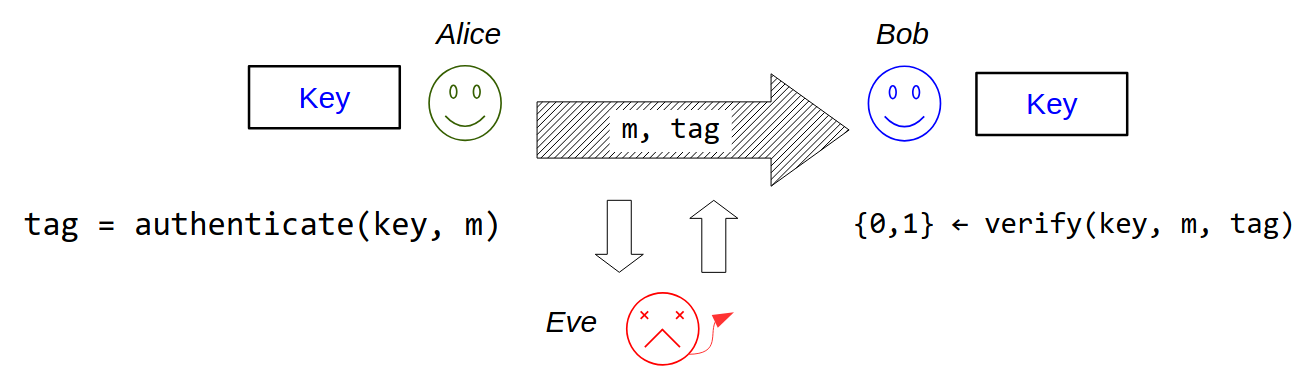
\includegraphics[width=0.55\textwidth]{img/mac_tag.png}
    \end{figure}

    L'integrità dell'informazione è condizione necessaria per l'autenticità, se l'attaccante può modificare il dato, allora può anche impersonificare il mittente del dato, violando l'autenticità.

    \smallskip

    È spesso confusa l'integrità del dato con la sua autenticità, nel contesto della sicurezza informatica noi cerchiamo l'autenticità - e quindi implicitamente l'integrità - per questo motivo andremo ad analizzare \textbf{\textit{authenticated encryption}}. È però fondamentale differenziare le due proprietà in quanto utilizzano schemi di crittografia differenti:
    \begin{itemize}[nosep]
        \item \textbf{\textit{Integrity}} utilizzo delle \textbf{funzioni hash}.
        \item \textbf{\textit{Authenticity}} utilizza i \textbf{\textit{Message Authentication Code - MAC}}, per ora andremo ad analizzarli nell'ambito della crittografia simmetrica.
    \end{itemize}

    \textcolor{red}{\textbf{\textit{Hash function \& cryptographic integrity guarantees}}} \\
    Andiamo, velocemente, ad analizzare quelle situazioni in cui è richiesta \textbf{\textit{integrità}} fuori dai requisiti di crittografia: come ad esempio modifiche al dato per errori di trasmissione o per guasti - normalmente scaturite da fenomeni fisici - per i quali sono presenti molteplici algoritmi, tra i quali: \textbf{\textit{parity}}, \textbf{CRC}, \textbf{\textit{checksum}}. In questo caso è possibile modellare la tipologia di attaccante come un \textbf{attaccante irrazionale} (perdita di bit randomici o a raffica). \\
    Nei settaggi di crittografia moderna, l'attaccante è sempre \textbf{razionale} e conosce gli \textbf{algoritmi crittografici} e si comporta di conseguenza, grazie al requisito di \textbf{\textit{cryptographic integrity-protection}} anche se noti i dati di base non deve essere capace di trovare una soluzione al problema nonostante l'assenza di una chiave condivisa. Anche in questo caso è presente la sicurezza computazione ma viene applicata in maniera differente.

\end{flushleft}

\section{Hash Function}

\begin{flushleft}

    \textcolor{red}{\textbf{Cryptography Hash Function}}: una funzione hash $H$ viene definita come: 

    {\centering
        $H : \{0, 1\}^* \mapsto \{0, 1\}^n$
    \par}

    ovvero è possibile mappare una quantità arbitraria di bit - nelle moderne funzioni hash $*$ è così ampio che può anche considerato a $\infty$ - in una sequenza fissata (piccola) - che è definita dall'algoritmo. L'ouput di $H$ viene chiamato \textbf{\textit{digest}} - le funzioni di hash esistono anche per scopi non prettamente crittografici. La dimensione di \textbf{n} è scelta in maniera tale che sia altamente improbabile che due input differenti generino lo stesso output, in questo modo il \textit{digest} è un informazione ``piccola'' che rappresenta univocamente l'informazione contenuto nel dato. È possibile paragonare il comportamento ad una \textbf{funzione di compressione pseudorandom}

    {\centering
        $m_1 \neq m_2 \longleftrightarrow d_1 \neq d_2$
    \par}

    Il comportamente delle funzioni hash - \textbf{PRF} - può essere applicato anche a circostante non crittografiche, ad esempio: \textbf{MD5} è una funzione hash deprecata, ma viene utilizzata per identificare in maniera univoca i commit su git. È possibile anche utilizzarle come \textbf{primitive} per costruire blocchi per altri schemi crittografici, ad esempio: alcuni \textbf{MAC} si basano su delle \textit{hash function} ed anche alcune \textbf{\textit{Key Derivation Function - KDF}}.

    \medskip

    In base al tipo di applicazione che stiamo utilizzando bisogna che la funzione hash sia resistente a diversi \textbf{\textit{attack model}}, tutti quanti, se no viene definita \textbf{deprecata}.

    \textcolor{red}{\textbf{\textit{Attack Models} Differenti}}
    \begin{center}
        \begin{minipage}[c]{0.75\textwidth}
            \begin{itemize}[nosep]
                \item \textbf{\textit{One Way}} anche nota come \textbf{\textit{first pre-image resistance}}, deve essere \textbf{efficiente} calcolare $H(m) = d$, ma \textbf{inefficiente} calcolare la funzione opposta, ovvero risalire a $m = H^{-1}(d)$
                \item \textbf{\textit{Second pre-image Collision Resistant}} ovvero dato un messaggio $m_1$ è \textbf{inefficiente} trovare un messaggio $m_2$ tale che $H(m_1) = H(m_2)$
                \item \textbf{\textit{Collision Resistant}} è \textbf{inefficiente} trovare una coppia di messaggi - \textbf{arbitrari} - $m_1$ e $m_2$ tale che $H(m_1) = H(m_2)$
            \end{itemize}
        \end{minipage}
        \hfill
        \begin{minipage}[c]{0.1\textwidth}
            \centering
            \begin{tikzpicture}[scale=1]
                \node[rotate=270, anchor=south, text=red] at (0,2.2) {\textbf{stronger attack models}};
                \draw[<-, thick, black] (0,-0.5) -- (0,5.0);
            \end{tikzpicture}
        \end{minipage}
    \end{center}

    \textcolor{red}{\textbf{\textit{First pre-Image Resistance}}}: dato un \textit{digest}, calcolarsi il dato. È tipicamente associato a \textbf{garanzie di confidenzialità} - può essere applicato a schemi di \textbf{KDF}.

    \begin{figure}[h]
        \centering
        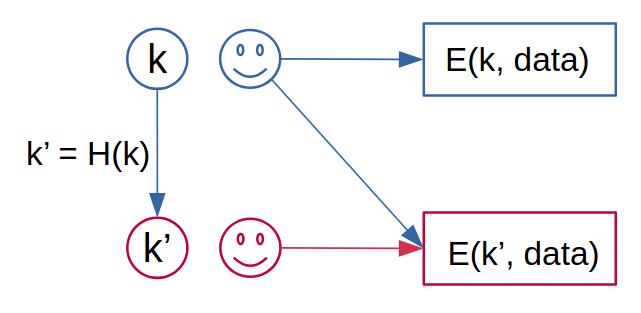
\includegraphics[width=0.45\textwidth]{img/one_way.png}
    \end{figure}
    
    Dato in input una chiave, ottengo in output un'altra chiave $k' = H(k)$ in questo caso cosa dovrebbe rompere Eve per riuscire a decifrare? In questo contesto anche se $H$ \textbf{non} è \textit{collision resistance} non è di interesse infatti anche se si trovasse un $k'' \; \text{t.c.} \; k' = H(k'') \rightarrow k \neq k''$ e quindi Eve non riuscirebbe a rompere lo schema crittografico di cifratura, l'unico modo per Eve di ottenere il dato in chiaro è riuscire a trovare una funzione $H^{-1} \; \text{t.c.} \; k = H^{-1}(k')$ e utilizzarla per decifrare le informazioni di Alice - ci basta: \textbf{\textit{One Way}}. \\
    L'unica limitazione è che se l'input $k$ è debole e quindi vulnerabile a \textit{brute-force} allora sarebbe possibile eseguire una ricerca esaustiva nell'insieme delle chiavi - \textbf{\textit{HKDF}}.

    \medskip

    \textcolor{red}{\textbf{\textit{Second pre-Image Collision Resistance}}}: dato un $d$ e un $m$ tale che $d = H(m)$ trovare un valore $m' \; \text{t.c.} \; d = H(m')$ è tecnicamente richiesta per gli \textbf{\textit{authentication schemes}} ad esempio nel contesto di \textbf{\textit{Keyed Hash Function}} - per l'offuscamento di password su DB - infatti riuscendo o a trovare $H^{-1}$ o trovando un'altro valore $m'$ che generi lo stesso \textit{digest} è possibile bypassare il controllo.
\end{flushleft}

\begin{boxA}
    \textcolor{orange}{\textbf{Esempio}}: \textbf{Download di dati}

    \medskip

    {\centering
        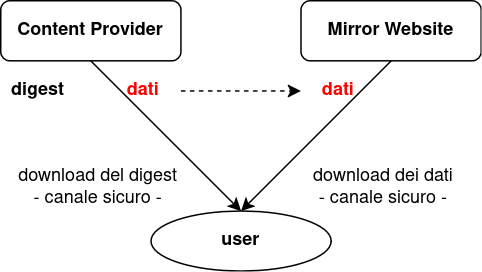
\includegraphics[width=0.45\textwidth]{img/hash_es.png}
    \par}

    Quando un sito mette a disposizione dei dati per il download - ad esempio un \textit{*.iso}, normalmente il contenuto per il download è disponibile su un \textit{server mirror}, quindi il \textit{provider} si calcola il \textit{digest} $d = H(m)$ e poi fa l'upload del contenuto sul \textit{server mirror}. L'utente si scarica il contenuto dal \textit{server mirror} e scarica il \textit{digest} dal \textit{provider}, successivamente calcola l'hash del dato scaricato $d_u = H(m_d)$ se e solo se $d_u = d$ accetta il dato scaricato.

    \smallskip

    In questo caso la funzione hash $H$ deve rispettare la ``normativa'' di sicurezza \textit{second pre-image collision resistance} in quanto il messaggio iniziale - la nostra \textit{*.iso} - viene fornita dal \textit{server mirror}. L'attaccante vincerebbe se riuscisse a trovare un messaggio $m_a \; \text{t.c.} \; H(m_d) = H(m_a)$ e contemporaneamente quel messaggio dovrebbe contenere un \textit{payload} malevolo. Solo in quel caso l'utente lo scaricherebbe il messaggio e la funzione di verifica - chiamata \textbf{\textit{verify}} - andrebbe a buon fine e quindi l'utente accetterebbe il nuovo messaggio.
\end{boxA}

\begin{flushleft}
    \textcolor{red}{\textbf{\textit{Collision Resistance}}}: riuscire ad ottenere, arbitrariamente, due messaggi $m_1$ e $m_2$ tali che $H(m_1) = H(m_2)$ è la più forte come garanzia di sicurezza, nel caso dovesse mancare, la funzione hash sarebbe molto facile da violare.
\end{flushleft}

\begin{boxA}
    \textcolor{orange}{\textbf{Esempio}}

    \medskip

    {\centering
        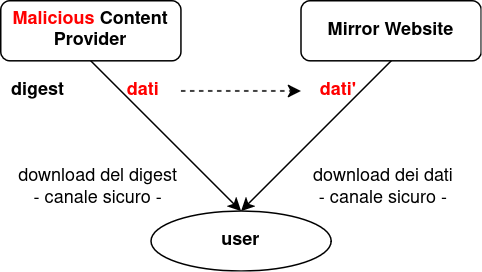
\includegraphics[width=0.45\textwidth]{img/hash_es_2.png}
    \par}

    Il \textit{provider} è malevolo e riesce a trovare due messaggio $m$ e $m'$ tali che $H(m) = H(m')$ a questo punto fa l'upload del messaggio malevolo sul \textit{server mirror}, l'utente che si scarica riesce a verificare la correttezza del \textit{digest}.
\end{boxA}

\begin{flushleft}
    \textcolor{red}{\textbf{\textit{Hash Function Security Parameters}}}: il \textbf{parametro di sicurezza} delle funzioni \textit{hash} è la \textbf{lunghezza del \textit{digest}} in quanto rappresenta le prossibili combinazioni di $n$ bit, ovvero i possibili valori prodotti dalla funzione \textit{hash} ($2^n$). Come discusso nel paragrafo di sicurezza computazionale, il valore di $n$ deve essere scelto considerando l'attacco noto più efficiente, analizzando anche il numero di operazioni richieste per trovare una collisione. 

    \smallskip

    Una funzione hash sicura è quello in cui l'attacco più efficiente per trovare una collisione è il \textbf{\textit{Birthday Attack}} che richiede $2^{n/2}$ ovvero la probabilità di trovare una collisione è del $50\%$ su $N$ ($\sqrt{N}$)

    \medskip

    Alcune delle più popolari funzioni hash:
    \begin{itemize}[nosep]
        \item \textbf{md5}: ad oggi deprecata, molto facile trovare delle collisioni.
        \item \textbf{sha1}: anche questa ad oggi deprecata, vi sono trovate delle collisioni. 160bit di \textit{digest}.
        \item \textbf{sha2}: sha1 ``potenziata'' ha diverse lunghezze del \textit{digest} in base alla versione: \textbf{sha224}, \textbf{sha256}, \textbf{sha384} e \textbf{sha512}.
        \item \textbf{sha3}: è stata implementata con una primitiva differente rispetto a sha1 e sha2, è stata standardizzata ufficialmente nel 2015, ha le stesse sottoversioni del sha2.
        \item \textbf{blake2}: utilizza come primitiva \textbf{chacha} non è ancora stata standardizzata dal NIST ma è molto popolari in certi ambienti, ad esempio, quello del \textit{software open source}.
    \end{itemize}

    Sia le funzioni \textbf{\textit{hash}} che le funzioni \textbf{\textit{mac}} vengono definite come funzioni con un solo input, ma è possibile concatenare più input, ma bisogna farlo in maniera sicura.

    {\centering
        $H('builtin' || 'security') = H('built' || 'insecurity') = H('builtinsecurity')$
    \par}

    Concatenare i risultati cercando di rendere univoco l'output:
    \begin{itemize}[nosep]
        \item utilizzando \textbf{caratteri speciali} per concatenare, se possibile: considersiamo che il carattere $;$ non sia ammesso come input allora sarà possibile concatenare gli input come: $d = H('builtin' \; || \; ';' \; || \; 'security')$
        \item \textbf{esplicitando} la \textbf{lunghezza dell'input}: $d = H('7buildinsecurity')$ 
    \end{itemize}
\end{flushleft}

\section{Message Authentication Code}

\begin{flushleft}
    Il destinatario può rilevare se il messaggio non è stato mandato da un mittente legittimo, che nel caso lo si andasse a definire all'interno della crittografia simmetrica, identificherebbe colui che conosce il segreto condiviso. Il \textbf{MAC} è una funzione che ha due input: la chiave e il message e come output un \textbf{\textit{tag}}.

    {\centering
        \textbf{tag} = \textbf{MAC}(\textit{key}, \textit{message})
    \par}

    La funzione \textbf{\textit{verify}} è simile a quella delle funzioni hash, ma include come input anche la chiave simmetrica.

    {\centering
        $\{0, 1\} \leftarrow$ \textbf{verify}(\textit{key}, \textit{message}, \textit{tag})
    \par}

    Il \textbf{MAC} permette a Bob di verificare che il messaggio è stato generato da Alice.
\end{flushleft}

\begin{flushleft}
    \textcolor{red}{\textbf{\textit{Attack Models for MAC}}}

    \medskip

    \begin{minipage}[c]{0.45\textwidth}
        \centering
        \textbf{\textit{Existential Forgery for Passive Eavesdropper}} \\
        L'attaccante osserva coppie $(m_i, t_i)$ trasmesse tra gli attori benevoli (Alice e Bob) ed è capace di \textit{forgiare} una nuova coppia $(m', t')$ mai inviata e l'attacco ha successo nel caso in cui il messaggio venga accettato.

        \smallskip

        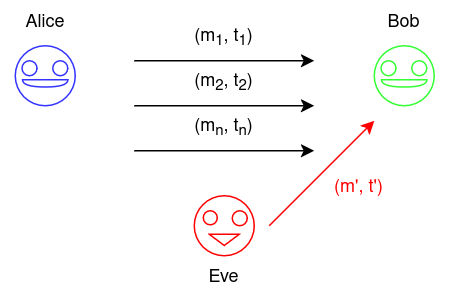
\includegraphics[width=\textwidth]{img/mac_am_1.png}
    \end{minipage}
    \hfill
    \begin{minipage}[c]{0.45\textwidth}
        \centering
        \textbf{\textit{Existential Forgery for Chosen Message}} \\
        In questo caso l'attaccante controlla i messaggi che vengono autenticati, quindi sceglie $n$ volte un messaggio $m_i$ e osserva il tag generato $t_i$ a quel punto se riesce a generare una nuova coppia $(m', t')$ non ancora inviata che verrà accettata l'attacco avrà avuto successo.

        \smallskip

        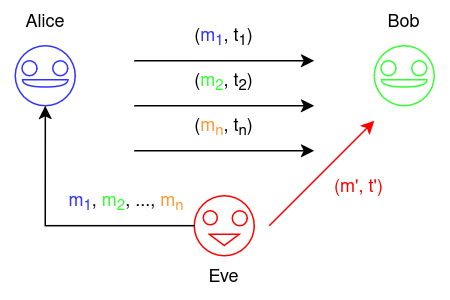
\includegraphics[width=\textwidth]{img/mac_am_2.png}
    \end{minipage}

    \smallskip

    \textcolor{red}{\textbf{\textit{MAC: Security Parameters}}}:
    \begin{itemize}[nosep]
        \item la \textbf{lunghezza della chiave}: l'attacco più efficiente deve essere quello di \textit{brute force}.
        \item la \textbf{lunghezza del \textit{tag}}: permette di determinare la dimensione del dato o il numero di messaggi autenticabili con la stessa chiave (dipende dal tipo di \textbf{\textit{MAC scheme}} che si vuole utilizzare). Ricordiamo che il \textit{tag} è \textbf{\textit{overhead}} sul messaggio e quindi è possibile minimizzarlo ma aggiungendo a livello di protocollo altri fattori di sicurezza. 
    \end{itemize}

    La scelta del \textbf{MAC} dipende dai requisiti nei quali va applicato. Disponibilità software (presenza di librerie), disponibilità hardware (accelleratore hardware) e l'abilità di soddisfare requisiti degli schemi (creare \textit{nonce}). Ogni tipologia di \textbf{MAC} offre un diverso \textit{trade-offs} in termini di: lunghezza e numero di messaggi, modelli di attacco e lunghezza del tag consentita.

    \medskip

    Consideriamo i \textbf{MAC} all'interno di una situazione di \textcolor{red}{\textbf{\textit{Replay Attack}}}. Abbiamo detto che il \textbf{MAC} può garantire che il \textit{tag} sia stato creato con una certa \textbf{chiave simmetrica}, ma nel contesto in cui siamo Eve re-invia lo stesso messaggio che ha inviato Alice a Bob, che è valido, perché creato da Alice - se Alice e Bob fossero due banchieri e Alice inviasse un messaggio con scritto "Aggiungi 1000 euro nell'account di Carlo". Con queste tipologie di attacco utilizzando la crittografia è difficile arginarle, è possibile però metterci una ``pezza'' lato architetturale (a livello \textbf{trasporto} o \textbf{applicazione}) ad esempio aggiungendo un \textbf{contatore univoco} al messaggio:
    
    {\centering
        \textbf{m} = (id=n, data), tag
    \par}

    Se consideriamo che la comunicazione sia \textit{full-duplex} - \textbf{\textit{Reflection Attacks}} - la possibilità che il messaggio venga inviato al mittente dello stessa e che venga verificato il \textit{tag} non è nulla, quindi si è aggiunto un bit di direzione del messaggio:

    {\centering
        \textbf{m} = (id=n, dir=val, data), tag
    \par}

    Il bit di direzione è aggiunto come \textbf{metadato} per un verifica ulteriore da parte del destinatario. È anche possibile utilizzare una difesa diversa, gestire la comunicazione \textit{full-duplex} come due \textbf{comunicazioni sicure \textit{half-duplex}} quindi utilizzare due \textbf{chiavi differenti} entrambe condivise, ma se invia Alice, verrà utilizzata $k_1$, se invia Bob $k_2$.

    \medskip

    \textcolor{red}{\textbf{\textit{MAC \& Hash function}}} \\
    Consideriamo un \textit{tag} generato in questo modo: \textbf{H}(\textbf{key} || \textbf{message}), ovvero ci calcoliamo l'hash di una stringa generata concatenando la chiave con il messaggio. Si potrebbe pensare che se la funzione hash è \textit{collision resistance} un'attaccante non riuscirebbe a calcolare un \textit{digest} la cui pre-immagine è (parzialmente) sconosciuta. In verità questo tipo di costrutto è vulnerabile al \textbf{\textit{length extension attack}} in quanto molte funzioni hash si basano sulla primitiva di \textbf{\textit{Merkle-Damgard}} (non vale per \textbf{sha3})
\end{flushleft}

\begin{boxA}
    \textcolor{red}{\textbf{\textit{Merkle-Damgard Design}}} \\

    {\centering
        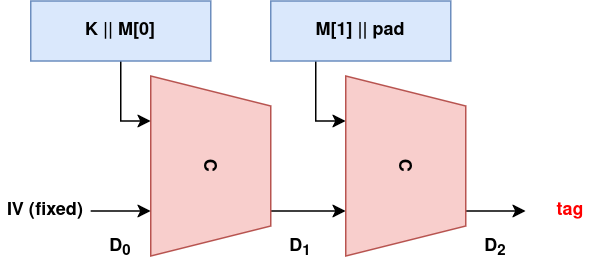
\includegraphics[width=0.45\textwidth]{img/hash_md.png}
    \par}

    È la primitiva che viene utilizzata da \textit{hash function} come \textbf{md5}, \textbf{sha1}, \textbf{sha2}. Considerando la figura, vediamo che:
    \begin{itemize}[nosep]
        \item \textbf{K} è il segreto.
        \item \textbf{M[0]} e \textbf{M[1]} è pubblico.
        \item la costruzione del \textbf{pad} è pubblica.
        \item $D_2$ è pubblico (\textbf{\textit{tag}})
    \end{itemize}
    In questa circostanza l'attaccante vince se riesce a generare un \textit{tag} valido per un certo messaggio arbitrario senza conoscere la chiave \textbf{K}. Noi (come attaccante) sappiamo che il \textit{tag} è generato \textbf{H}(\textbf{key} || \textbf{message}) dove \textbf{K} è un segreto con una data lunghezza \textbf{l} fissata, noi vogliamo calcolare un certo \textit{tag'} che venga generato \textbf{H}(\textbf{key} || \textbf{message} || \textbf{message'}).
    \begin{enumerate}[nosep]
        \item Consideriamo di utilizzare la stessa \textit{hash function}, e di ripristinare il suo stato interno come, quindi ponendo come nostro \textbf{IV} il \textit{tag} generato dalla computazione legittima, ma è necessario impostare anche il punto iniziale da dove andare a calcolare il \textbf{pad'} e deve essere pari a $len(K) + len(M) + len(pad)$.
        \item Inviamo come messaggio \textbf{M || pad || M'} e come tag quello appena calcolato \textbf{\textit{tag'}}.
        \item il destinatario calcolerà \textbf{H}(\textbf{K} || \textbf{pad} || \textbf{M} || \textbf{pad} || \textbf{M'}) e produrrà lo stesso \textit{tag'} 
    \end{enumerate}
\end{boxA}

\begin{flushleft}
    \textcolor{red}{\textbf{\textit{HMAC}}}: è un MAC che viene costruito con alla base una funzione hash (alcune volte chiamato \textbf{\textit{keyed-hash function}}), è necessario che mantenga due requisiti funzionali:
    \begin{itemize}[nosep]
        \item il \textbf{MAC} deve essere sicuro fintanto che la primitiva hash su cui è costruito è \textit{collision resistance}.
        \item per molti degli scenari presi in considerazione è sufficiente una \textit{second pre-image collision resistance}
    \end{itemize}
    Viene definito come:

    {\centering
        \textbf{HMAC}(\textbf{K}, \textbf{M}) = \textcolor{blue}{\textbf{H(}}(Kp $\oplus$ opad) || \textcolor{red}{\textbf{H(}}(Kp $\oplus$ ipad) || (m)\textcolor{red}{\textbf{)}}\textcolor{blue}{\textbf{)}}
    \par}
    Dove: 
    \begin{itemize}[nosep]
        \item \textbf{K} è un segreto a lunghezza variabile, mentre \textbf{Kp} è la sua versione \textit{zero-padded}.
        \item \textbf{opad}(\textbf{\textit{outer padding}}) e \textbf{ipad}(\textbf{\textit{inner padding}}) sono costanti con un elevata distanza di Hamming (ovvero che le posizioni di bit diversi sono elevate), utilizzate per consentire alle due funzioni hash di utilizzare chiavi diverse.
    \end{itemize}
\end{flushleft}

\begin{flushleft}
    Andiamo a considerare i \textbf{MAC} costruiti su \textit{block cipher}, il primo e il più semplice per costruire un \textbf{MAC} basato su \textit{block cipher} fu quello di utilizzare la \textbf{CBC} \textit{mode of operation} e utilizzare come \textit{tag} il testo cifrato dell'ultimo blocco.

    {\centering
        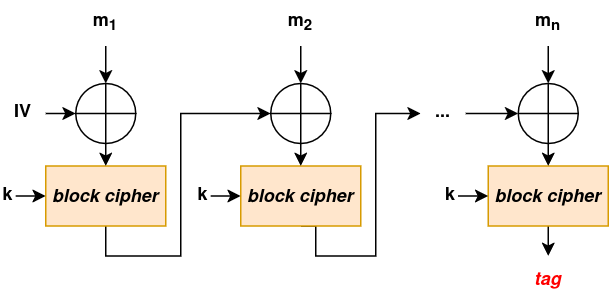
\includegraphics[width=0.45\textwidth]{img/cbc_mac.png}
    \par}

    È possibile \textit{forgiare} un messaggio, da parte di un attaccante, infatti dato \textbf{(m, t)} e \textbf{(m', t')}, un \textcolor{red}{\textbf{CBC-MAC}} producerà \textbf{t'} per un messaggio costruito come: \textbf{m || t $\oplus$ m' || m'}.

    \medskip
    
    \textcolor{red}{\textbf{\textit{CMAC}}} è il successore del \textbf{CBC-MAC} utilizza come primitiva \textbf{AES-SIV}(\textbf{CTR-CMAC}), lo schema è molto simile ma aggiunge due operazioni sull'ultimo blocco prima di utilizzarlo. Lo schema deriva due chiavi $k_1$ e $k_2$ dalla chiave originale e una delle due viene \textit{xorata} con l'ultimo blocco del messaggio $m_n$ (\textbf{\textit{tweak block}}) prima di utilizzare il blocco del \textbf{CMAC}.

    {\centering
        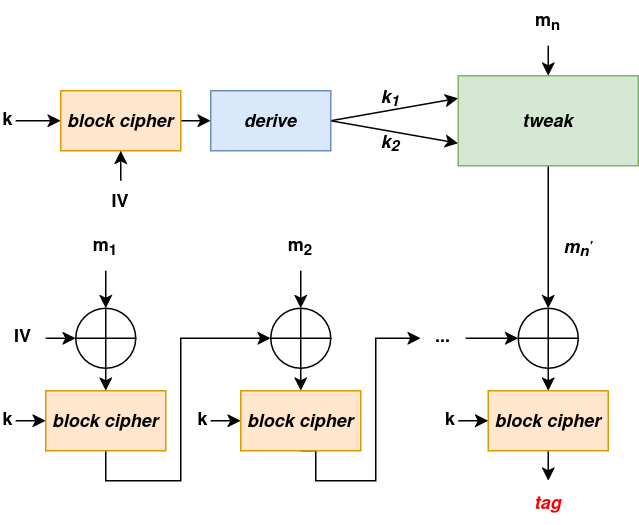
\includegraphics[width=0.45\textwidth]{img/cmac.png}
    \par}

    \newpage

    \textcolor{red}{\textbf{\textit{UHF - Universal Hash Function}}} si riferisce ad una \textbf{\textit{keyed hash function}} che prende due input: una chiave \textbf{k} e un messaggio \textbf{m}. Questa funzione garantisce che la probabilità - che dati due messaggi distinti $m_1$ e $m_2$ - di avere $UHF(m_1) = UHF(m_2)$ è \textbf{trascurabile}. Un'implementazione popolare per una funzione \textbf{UHF} è quella basata su \textbf{polinomi modulo p} (con \textbf{p} primo):
    \begin{itemize}[nosep]
        \item scegliamo un primo \textbf{p}
        \item consideriamo il messaggio $m$ come un vettore di interi in $\mathbb{Z}_p$ con un massimo di $n$ elementi: $m = [m_1, m_2, ..., m_n]$
        \item la funzione hash \textbf{H} viene calcolata utilizzando gli elementi di $m$ come coefficienti del polinomio $F(k)$:
        
        {\centering
            $H(k, M) = \overset{n}{\underset{i=1}{\sum}} (m_i \cdot k^i) \mod p$
        \par}

    \end{itemize}

    \medskip
    
    \textcolor{red}{\textbf{\textit{One-Message Polynomial evaluation MACs}}}: è possibile costruire un \textbf{MAC} partendo da delle \textbf{UHF}, consideriamo il messaggio $m = m_1, m_2, ..., m_n$

    {\centering
        $mac(m, k, r) = r + H(m, k) = r + \overset{n}{\underset{i=1}{\sum}} (m_i \cdot k^i) \mod p$
    \par}

    In questo caso il \textbf{MAC} è un polinomio di grado $n$, \textbf{p} è fissato ed è pubblico, se $m_i$ è 128bit allora $p > 128$. \textbf{k} e \textbf{r} vengono scelti randomicamente:
    \begin{itemize}[nosep]
        \item \textbf{k} lavora come la chiave per la computazione, può essere utilizzata per più messaggi.
        \item \textbf{r} ha la stessa funzionalità di un \textbf{\textit{nonce}} random, e bisogna utilizzarlo assolutamente per un unico messaggio, in questo caso \textbf{r} è \textbf{segreto}.
    \end{itemize}
    Nel caso in cui \textbf{r} venisse ripetuto per due \textit{tag}:
    \begin{align*}
        \mathbf{t_1} &= mac(m_1, k, r) = r + H(m_1, k) \\
        t_1 - r - H(m_1, k) &= 0 \\
        \mathbf{t_2} &= mac(m_2, k, r) = r + H(m_2, k) \\
        t_2 - r - H(m_2, k) &= 0
    \end{align*}

    \begin{align*}
        t_1 - \cancel{r} - H(m_1, k) &= t_2 - \cancel{r} - H(m_2, k) \\
        \overset{n}{\underset{i=1}{\sum}}(m_{1,i} \cdot k^i) + t_1 &= t_2 + \overset{n}{\underset{i=1}{\sum}}(m_{2,i} \cdot k^i) \\
        \overset{n}{\underset{i=1}{\sum}}((m_{1, i} - m_{2, i}) \cdot k^i) + t_1 - t_2 &= 0 \mod p
    \end{align*}
    In questo modo la chiave \textbf{k} è tra le radici del polinomio $m_2 - m_1 + t_1 + t_2$. 
    \smallskip
    È possibile estendere \textit{one-message poly MACs} ad un \textit{multi-message} utilizzando o una \textbf{PRF} oppure \textbf{PRP} (ad esempio un \textit{block cipher}), in questo modo, invece che utilizzare un valore di \textbf{r} random possiamo calcolarlo partendo da una chiave e un \textit{nonce}:

    {\centering
        $mac(m, k = \langle k_1, k_2 \rangle, n) = AES(n, k_1) + H(m, k_2)$
    \par}

    Se $k_1$ è segreta, un avversario, non sarebbe in grado di calcolarsi \textbf{AES}(n, $k_1$) anche se il valore $n$ fosse pubblico e non randomico, ma utilizzare lo stesso \textit{nonce} più volte esporrebbe $k_2$ e quindi romperebbe lo schema.

    \medskip

    \textcolor{red}{\textbf{\textit{GMAC}}} è basato su \textbf{AES-GCM} e in questo caso i rischi per la sicurezza in caso di errori di utilizzo sono molto più elevati a causa del comportamento lineare della funzione. Richiede un \textbf{\textit{unpredictable nonce}}, riutilizzare lo stesso \textit{nonce} per firmare messaggi diversi permette la \textbf{\textit{key recovery}}, in questo caso è molto importante utilizzare la variante \textbf{SIV} - molto più robusti a discapito delle \textit{performance} - come primivita dello schema (\textbf{AES-GCM-SIV}). La probabilità di successo in caso di attacco \textbf{aumenta} all'\textbf{aumentare della dimensione del messaggio}.

    \smallskip

    Non possiamo effettuare un'analisi a \textit{black-box} per definire come la dimensione del \textit{tag} influenzi il \textbf{livello di sicurezza}. Il dimensionamento richiede la conoscenza dello schema e le analisi sono parecchio complesse. Alcuni esempi:
    \begin{itemize}[nosep]
        \item \textbf{HMAC} e \textbf{CMAC}: è possibile mandare un numero di messaggi pari alla radice quadrata della dimensione del \textit{digest}
        \item \textbf{GHASH} (e \textbf{GMAC}): il numero dei messaggi è lineare con la dimensione del \textit{digest}, ma diminuisce rispetto alla dimensione di ogni messaggio.
        \item \textbf{Poly1305}: rappresenta un \textit{trade-off}, alto numero di messaggi dimensionalmente limitati.
    \end{itemize}
\end{flushleft}
\chapter{Security Guarantees \& Attack Model \\ \small{for Symmetric Encryption}}

\begin{flushleft}
    Ogni schema crittografico garantisce sicurezza contro un certo attaccante a condizione che siano soddisfatti certi requisiti:
    \begin{itemize}[nosep]
        \item dobbiamo decidere quale modello si adatta allo schema considerato.
        \item dobbiamo considerare i vincoli funzionali e non.
    \end{itemize}

    Lo scopo finale dell'attaccante è quello di violare la \textbf{confidenzialità}, per ora abbiamo solo considerato un attaccante che non ha alcuna conoscenza \textbf{EAV}, ma a volte, l'attaccante può anche:
    \begin{itemize}[nosep]
        \item avere \textbf{conoscenza} aggiuntiva sul \textit{plaintext}.
        \item violare l'\textbf{integrità} di un vettore di attacco per ottenere delle informazioni.
        \item \textbf{interagire} con le parti fidate.
    \end{itemize}

    È importante ricordare che la confidenzialità nella crittografia moderna è modellata come \textbf{indistinguibilità} da una sequenza random. Infatti l'avversario vince nel caso in cui è capace di riconoscere un crittogramma da un messaggio random con una proabilità maggiore del $50\% + negl(n)$

    \smallskip

    Non è possibile enumerare tutti i possibili attacchi di uno scenario reale, quello che si prefigge la crittografia moderna è considerare alcuni modelli formali contro i quali la sicurezza degli schemi crittografici è comprovata. Il che ci permette di progettare il protocollo o l'applicazione andando a scegliere il modello più adatto al proprio scenario. Gli schemi di sicurezza sono dimostrati sicuri in presenza di determinati modelli di attacco.

    \medskip

    \textcolor{red}{\textbf{\textit{Attack Model}}} \\
    I modelli di attacco vegono pensati basandosi su due criteri di misura: \textbf{\textit{knowledge}} - che cosa sa l'avversario del nostro sistema - \textbf{\textit{attack surface}} - quali interfacce espone il nostro sistema che anche un avversario potrebbe utilizzare.

    \smallskip

    La crittografia formale moderna chiama queste interfacce \textbf{oracoli}, e normalmente andiamo a definirne di due tipologie:
    \begin{itemize}[nosep]
        \item \textbf{\textit{encryption oracle}}: l'attaccante può dare \textbf{input} all'oracolo e gli verrà ritornato un dato cifrato in \textbf{output} che corrisponde a \textbf{E}(input).
        \item \textbf{\textit{decryption oracle}}: è il duale dell'\textit{encryption oracle}.
    \end{itemize}
    Un vincolo aggiuntivo che si può aggiungere alla superficie di attacco quando si considera la distribuzione di un applicativo nel mondo reale è la tipologia di computazione che deve eseguire un attaccante: \textbf{\textit{online}} - l'interazione è con l'oracolo - e \textbf{\textit{offline}} - non è necessario consultare l'oracolo.

    \smallskip

    \textcolor{red}{\textbf{\textit{Attack Models} Differenti}}
    \begin{center}
        \begin{minipage}[c]{0.75\textwidth}
            \begin{itemize}[nosep]
                \item \textbf{\textit{Eavesdropper - EAV}} anche nota come \textbf{\textit{Ciphertext-Only Attack - COA}} l'avversario è passivo e non ha conoscenza sui crittogrammi che riesce ad intercettare.
                \item \textbf{\textit{Known-Plaintext Attack - KPA}} in questo caso l'avversario ha la conoscenza della coppia $(p_i, c_i)$
                \item \textbf{\textit{Chosen-Plaintext Attack - CPA}} 
                l'attaccante ha accesso ad una \textit{encryption interface} e quindi è in grado di cifrari messaggi arbitrari.
                \item \textbf{\textit{Non-Adaptive Chosen-Ciphertext Attack - CCA1}}: l'avversario ha accesso ad una \textit{decryption interface}, ma accesso limitato al risultato e limite sul numero di \textit{query} che può eseguire.
                \item \textbf{\textit{Adaptive Chosen-Ciphertext Attack - CCA2}}: l'avversario ha accesso ad una \textit{decryption interface} e anche al risultato e quindi modificare l'attacco in base ai risultati.
            \end{itemize}
        \end{minipage}
        \hfill
        \begin{minipage}[c]{0.1\textwidth}
            \centering
            \begin{tikzpicture}[scale=1]
                \node[rotate=270, anchor=south, text=red] at (0,2.2) {\textbf{stronger attack models}};
                \draw[<-, thick, black] (0,-3.0) -- (0,7.0);
            \end{tikzpicture}
        \end{minipage}
    \end{center}

    Come detto in precedenza la \textbf{confidenzialità} in crittografia modeerna equivale a dire che il crittogramma prodotto è \textbf{indistinguibile} da un \textit{random bitstring}. Associando \textbf{IND} ad un modello di attacco andiamo a definire una \textbf{garanzia di sicurezza} dello schema preso in considerazione, ad esempio dire che il nostro schema di crittografia è \textbf{IND-CPA} significa che lo schema è \textbf{indistinguibile da un \textit{random} contro un modello di attacco \textit{Chosen-Plaintext Attack}}.

    \smallskip

    \textcolor{red}{\textbf{IND-EAV (\textit{Indistinguishably under Eavesdropper Attack})}}: è la tipologia di attacco più debole, in quanto un attaccante non sa nulla. Eve è un attaccante passivo che osserva crittogrammi senza eseguire alcuna modifica su di essi e senza interagire con le parti fidate, ma soprattutto senza alcuna conoscenza del testo in chiaro.
\end{flushleft}

\begin{boxA}
    \textcolor{red}{\textbf{\textit{Semantic Security Games on IND-COA}}} \\
    Tutti i \textit{security games} per la confidenzialità sono basati sul concetto di \textbf{indistinguibilità}, un algoritmo eseguito dall'attaccante che ha come scopo di distinguere informazioni dal \textit{plaintext}. 
    
    \smallskip

    Nel modello di attacco \textbf{COA}, l'avversario legge i crittogrammi in transito e prova a indovinare il bit successivo. Riuscirà a vincere il gioco solo se ha un \textit{distinguisher} che indovina il bit corretto con una probabilità $ > 0.5$, nei moderni modelli di attacco, l'avversario non deve necessariamente ottenere la chiave di cifrazione o il contenuto effettivo del testo in chiaro affinché uno schema si consideri ``rotto''.
\end{boxA}

\begin{flushleft}
    \textcolor{red}{\textbf{IND-KPA (\textit{Indistinguishably under Know-Plaintext Attack})}}: Eve è un attaccante passivo che osserva i crittogrammi senza eseguire alcuna modifica su di essi e senza interagire con le parti fidate, ma può conoscere vecchie corrispondenze tra $m$ e $c$ o informazioni sullo spazio dei testi in chiaro, come la distribuzione statistica.
    
    \smallskip

    \textcolor{red}{\textbf{IND-CPA (\textit{Indistinguishably under Chose-Plaintext Attack})}}: è la sicurezza minima richiesta da tutti i moderni crittosistemi, l'attaccante viene modellato per avere accesso ad un \textit{encryption oracle}.

    {\centering
        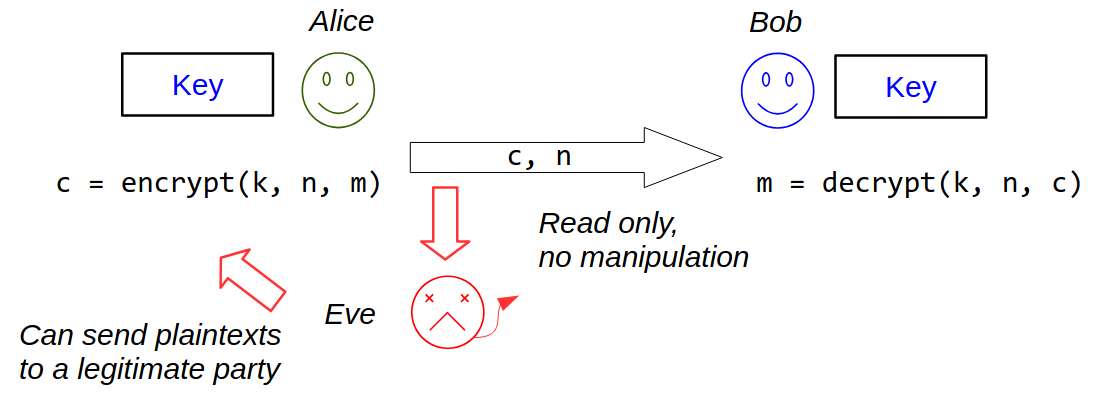
\includegraphics[width=0.45\textwidth]{img/ind_cpa.png}
    \par}

    \textbf{\textit{Security Games}}
    \begin{enumerate}[nosep]
        \item il \textbf{\textit{challenger}} genera una chiave segreta.
        \item l'\textbf{\textit{adversary}} sceglie due messaggi $m_0$ e $m_1$ della stessa lunghezza e gli invia al \textit{challenger}.
        \item il \textit{challenger} genera randomicamente un bit $b \leftarrow \{0, 1\}$ e genera $c = E(m_b)$ e lo invia all'avversario.
        \item l'\textit{adversary} analizza il crittogramma e può scegliere se ripetere gli step dal secondo o passare al quinto.
        \item l'avversario espone come output un valore $b \leftarrow \{0, 1\}$ in base a quale messaggio - se $m_0$ o $m_1$ - è il corrispondente di $c$.
    \end{enumerate}
    L'\textit{adversary} vince il gioco se è capace di riconoscere con una probabilità $ > 0.5\% + negl(l)$ a quale messaggio corrisponde il crittogramma ricevuto.
    
    \smallskip

    Qualunque schema \textbf{deterministico} è intrinsecamente vulnerabile a un attacco del tipo \textbf{IND-CPA}, in quanto basterebbe all'attaccante ripetere lo stesso messaggio per un più iterazioni consecutive e vincere, infatti schemi crittografici sono sicuri sotto la modellazione \textbf{\textit{Distinc Chosen-Plaintext Attack - DCPA}} che obbligano l'\textit{adversary} a scegliere una coppia di messaggi diversi per ogni iterazione del \textit{security game}. Crittografia deterministica è spesso implementata fornendo \textit{nonce} o \textit{IV} fissi (costanti) allo schema, cercando di evitare schemi che sono vulnerabili contro \textit{re-use} di \textit{nonce} o \textit{IV} oppure preferendo schemi che utilizzano \textbf{SIV}. \\
    \textbf{\textit{Deterministic Encryption with Associated Data - DAEAD}} framwork.
\end{flushleft}

\begin{boxA}
    \textcolor{red}{\textbf{IND-CPA e il requisito di impredicibilità dell'IV in CBC}}
    \begin{itemize}[nosep]
        \item \textit{adversary}: sceglie un $m$ che ha lunghezza pari alla \textit{block size} del \textit{block cipher} e lo invia.
        \item \textit{challenger}: sceglie un \textit{IV} e calcola il \textit{ciphertext} $c$, ritornando la coppia $(c, iv)$.
    \end{itemize}
    Facciamo ora un'\textbf{assunzione}: l'avversario conosce l'\textit{IV} successivo - \textbf{\textit{predictable IV}}. \\
    L'avversario può calcolarsi un messaggio $m'$ come $m' = (m \oplus iv \oplus iv')$ dove \textbf{\textit{iv'}} è l'\textit{IV} successivo che utilizzerà il \textit{challenger}. Se il \textit{challenger} cifrerà il messaggio 
    
    {\centering
        $c' = E(iv', m') = E(m' \oplus iv', k) = E(m \oplus \cancel{iv'} \oplus iv \oplus \cancel{iv'}, k) = E(m \oplus iv, k) = c$
    \par}
\end{boxA}

\begin{flushleft}
    \textcolor{red}{\textbf{\textit{IND-CCA1 (Indistinguishably under Chosen-Ciphertext Attack)}}} permette di difendersi contro attacchi attivi sul crittogramma. L'attaccante è capace di manipolare il \textit{ciphertext} al \textit{decryption oracle} (gli input dell'attaccante non sono adattivi per via della definizione data).

    {\centering
        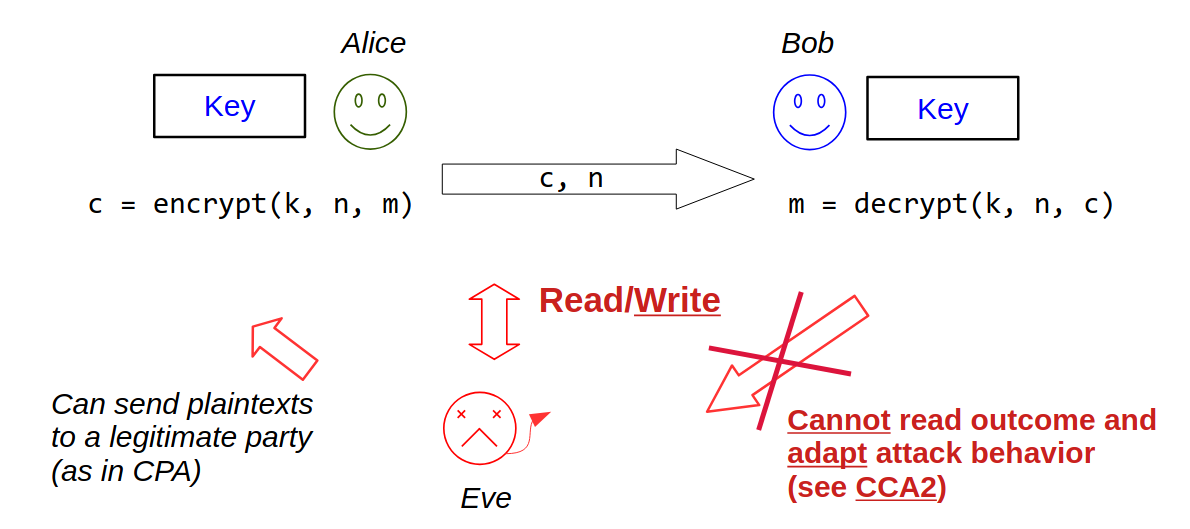
\includegraphics[width=0.45\textwidth]{img/ind_cca1.png}
    \par}

    \textbf{IND-CCA} coinvolge anche \textbf{modifiche al crittogramma} e \textbf{attacchi all'integrità per violare la confidenzialità}. 

    \smallskip

    \textcolor{red}{\textbf{\textit{Malleability}}} si riferisce alla capacità di un'attaccante di ricotruire quali bit del crittogramma sono influenzati dalla modifica di un bit nel testo in chiaro.

    \smallskip

    Un schema crittografico basato su \textcolor{red}{\textbf{\textit{stream cipher}}} viene definito \textbf{\textit{fully malleable}} in quanto una modifica nel testo cifrato in una certa posizione $c_i$ porta ad una modifica nel testo in chiaro nella medesima posizione $p_i$, ad esempio:
    \begin{enumerate}[nosep]
        \item \textit{flipping} il \textbf{bit di direzione} in uno protocollo di comunicazione per eseguire un \textbf{\textit{reflection attack}}.
        \item \textit{flipping} il numero di versione per effettuare un \textbf{\textit{downgrade attack}}.
    \end{enumerate}

    \smallskip

    Per ottenere una certa garanzia di \textbf{integrità} (senza utilizzare \textbf{MAC}) è necessario ricorrere a modalità di crittografia basate su \textit{block cipher}. Andiamo ad osservare il comportamento di uno schema crittografico basato su un qualunque \textit{block cipher} ma che abbia come \textit{mode of operation} \textbf{CBC}, in questo caso analizzando lo schema per decifrare un crittogramma generato, ad esempio, con \textbf{AES-CBC} è fattibile modificare l'\textit{IV}.

    {\centering
        
\includegraphics[width=0.45\textwidth]{img/ind_cca1_cbc.png}
    \par}

    Assumiamo che l'attaccante conosca il testo originale $p$ e voglia che in decifrazione venga generato il testo $p'$, nel \textbf{primo blocco}, allora sarebbe possibile calcolarsi un \textit{IV} tale che $IV' = (IV \oplus p \oplus p')$ e sostituire l'\textit{IV} originale con quello generato, in quel caso il primo blocco sarebbe $p'$ e i restanti blocchi rimerrebbero invariati.

    \medskip

    \textcolor{red}{\textbf{\textit{IND-CCA2 (Indistinguishably under Adaptive Chosen-Ciphertext Attack)}}} difende da attacchi attivi iterati e potenzialmente illimitati (l'attaccante è ancora \textbf{polinomiale}), in cui l'attaccante adatta i suoi attacchi in base alla risposta di Bob. L'attaccante invia un testo cifrato manipolato al \textit{decryption oracle}.

    {\centering
        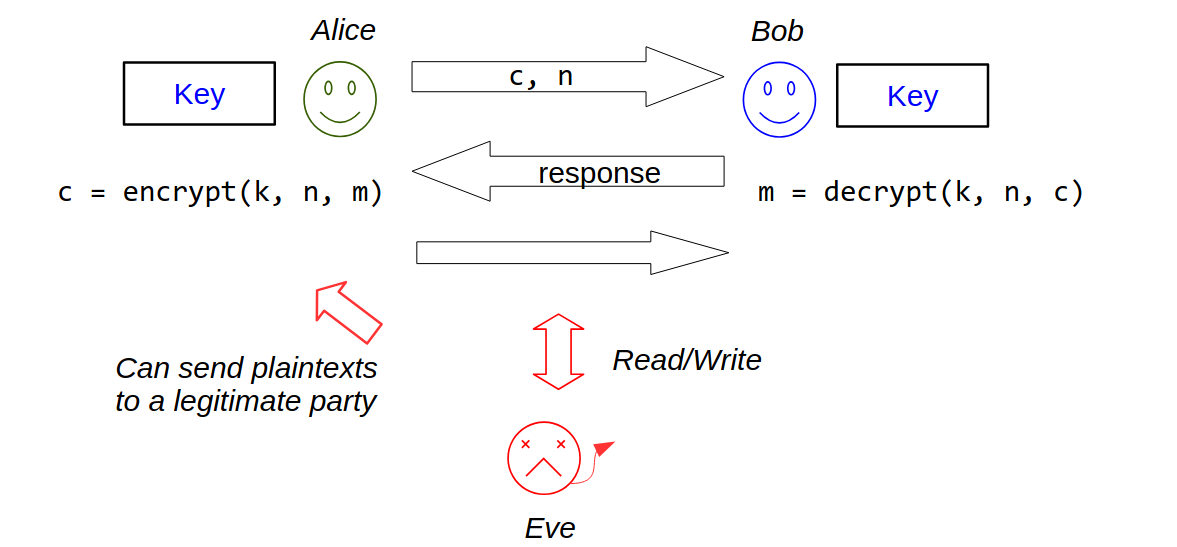
\includegraphics[width=0.45\textwidth]{img/ind_cca2.png}
    \par}
\end{flushleft}

\begin{boxA}
    \textcolor{red}{\textbf{\textit{Padding Oracle Attack}}} \\
    Consideriamo un attacco alle funzioni di \textbf{decifrazione} e \textbf{\textit{unpadding}}, l'attacco ha successo se riusciamo a generare un crittogramma che decifrandolo ha la struttura del \textit{padding} corretto. Gli attacchi al \textit{padding} mirano a manipolare un blocco di un crittogramma $c[i]$ per manipolare il blocco successivo di \textit{plaintext} $p[i+1]$. È simile alla manipolazione dell'\textit{IV} ma in questo caso andiamo a considerare gli ultimi due blocchi del \textit{ciphertext}, modificare il penultimo blocco per manipolare l'ultimo. In questo caso non abbiamo la certezza di come manipolare il crittogramma, ma possiamo \textit{guessare} - questo comporta che, in caso, di un unico tentativo ci siano probabilità trascurabili di successo, se avessimo più tentativi rientraimo nei \textbf{\textit{CCA2 attacks}}.
\end{boxA}

\begin{figure}[h]
    \begin{lstlisting}[mathescape=true]
import string

for character in string.printable:
    c[-2][-1] = character
    p[-1] = c[-2] $\oplus$ D(c[-1])

    if p[-1] has valid padding:
        attack ok
    else:
        attack failed
        \end{lstlisting}
        \label{lst:padding_oracle}
\end{figure}

\begin{boxA}
    Fissiamo \textbf{X} come il \textit{forged ciphertext} e con $\mathbf{X}_n$ l'$n$-simo \textbf{LSB}, \textbf{P} è il \textit{plaintext} originale e \textbf{T} l'output della funzione di decifrazione.
    \begin{enumerate}[nosep]
        \item impostiamo $n=1$ e $\mathbf{X}_n = 0$
        \item eseguiamo la \textit{decryption query} con $D(iv=X, \text{ciphertext}=V)$ e osserviamo la risposta:
        \begin{itemize}[nosep]
            \item \textbf{errore}: il crittogramma decifrato non ha il \textit{padding} valido, quindi $\mathbf{X}_n += 1$ e ripetiamo dal passo 2.
            \item \textbf{ok}: attacco andato a buon fine (tentativi massimo: 256, 128 in media), procediamo al punto 3.
        \end{itemize}
        \item segnamo $\mathbf{X}_n$ come $\mathbf{X}_{n,n}$
        \item se $n=16$ procediamo al passo 5, se no definiamo 
        
        {\centering
            $\mathbf{X}_{m, (m+1)} = [\mathbf{X}_{m,m} \oplus m \oplus (m+1)] \forall \; m \; \in [1, n]$
        \par}
        
        e $n += 1$ e ripetiamo dal passo 2.
        \item in fine possiamo decifrare il \textit{plaintext} originale, nell'ultimo blocco, calcolando:
        
        {\centering
            $P = C \oplus X \oplus [16]$
        \par}

        Dove $[16]$ è un blocco di padding nello standard \textbf{PKCS\#7}
    \end{enumerate}
    Questo attacco funziona perché:
    \begin{itemize}[nosep]
        \item \textbf{V} non viene mai modificato e quindi anche \textbf{T} che è sconosciuto.
        \item la decifratura non modificata esegue: $T \oplus C = P$.
        \item il \textit{padding oracle} ci permette di calcolare \textbf{X} in modo tale che $(T \oplus \mathbf{X}) = [16]$.
        \item $T = (\mathbf{X} \oplus [16])$ e $P = (C \oplus T) = (C \oplus C \oplus [16])$
    \end{itemize}
\end{boxA}

\newpage

\begin{flushleft}
    In questo caso non riuscire a sfruttare la \textbf{malleabilità} del sistema implicherebbe l'impossibilità di effettuare questo tipo di attacco, infatti la probabilità di indovinare il \textbf{padding} di dimensione $n$ sarebbe in media $2^{8n + 1}$ che è \textbf{inefficiente} in $n$. Siccome però in questo caso siamo capaci di sfruttare la malleabilità l'algoritmo abbassa il suo costo a $2^{8 - 1} \cdot n$ tentativi per un padding di dimensione $n$. Per \textbf{AES} sono necessarie all'incirca $\simeq 2000$ iterazioni per decifrare un blocco, è possibile decifrare l'intero crittogramma andando a \textbf{troncare} il crittogramma all'ultimo blocco. 
    
    \smallskip

    In alcuni casi potrebbe essere necessario gestire i falsi positivi del caso 2, al passaggio $n$ potremmo trovare un padding di dimensione $n' > n$
\end{flushleft}

\begin{flushleft}
    \textcolor{red}{\textbf{\textit{Authenticated Encryption}}}: tutti quelli schemi di crittografia che sono resistenti a modelli di attacco \textbf{IND-CCA2} verranno chiamati \textit{authenticated encryption scheme} ovvero schemi che non sono malleabili e che quindi nel caso di modifica, questa verrà rilevata, internamente utilizzano schemi di crittografia insieme a funzioni \textbf{MAC}, alcuni esempi:
    \begin{itemize}[nosep]
        \item \textbf{AES-GCM}: utilizza \textbf{AES-CTR} insieme ad un \textbf{GMAC}.
        \item \textbf{ChaCha20Poly1305}: utilizza \textbf{ChaCha20} insieme ad un autenticatore \textbf{Poly1305}.
        \item \textbf{AES-CCM}: utilizza \textbf{AES-CTR} insieme ad un \textbf{CMAC}.
    \end{itemize}
    Un esempio è quello di \textcolor{red}{\textbf{\textit{EFAIL vulnerability}}}.

    {\centering
        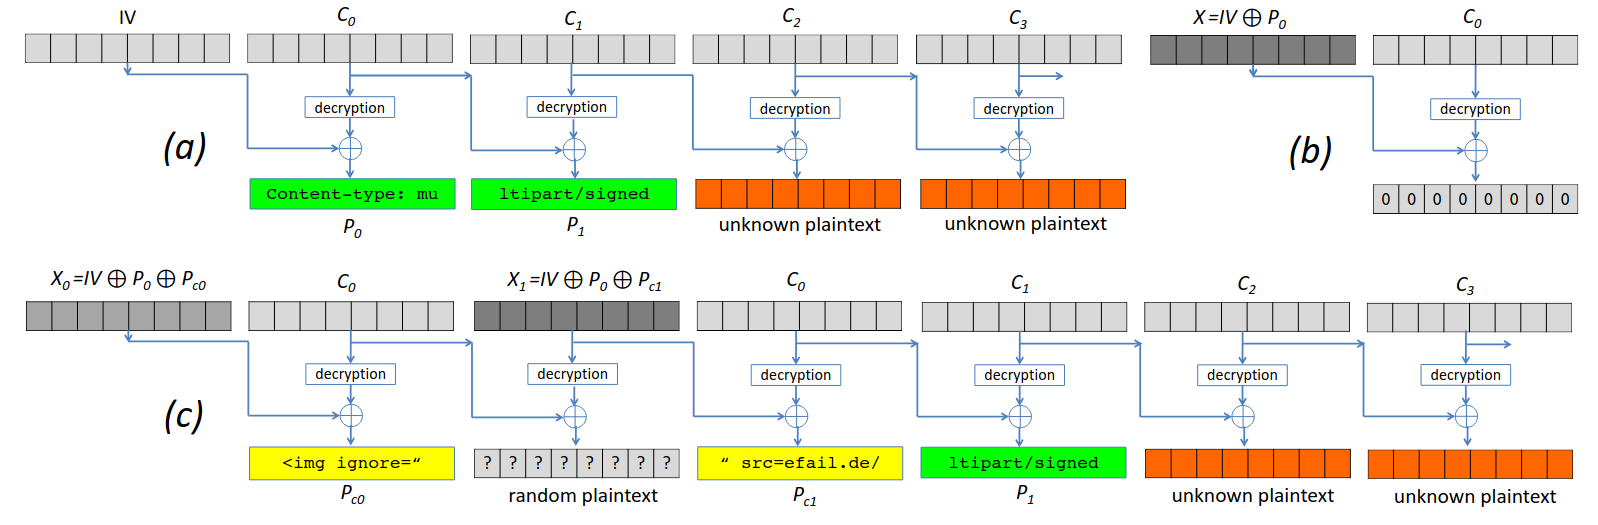
\includegraphics[width=\textwidth]{img/efail.png}
    \par}

    Protocolli crittografici: \textbf{s/MIME} + \textbf{OpenPGP} (\textbf{AES-CBC}), vettore di attacco: \textbf{\textit{Man in the middle}}. L'attaccante esponeva un servizio web che corrispondeva a \textbf{http://efail.de/ltipart/signed} e riuscia a leggere la mail in chiaro all'interno della richiesta.
\end{flushleft}
\chapter{Encryption schemes with integrity guarantees}

\section{IND-CCA2 Authenticated Encryption}

\begin{flushleft}
    La crittografia ``normale'' deve rispettare il requisito di \textbf{confidenzialità} contro un modello di attaccante del tipo \textbf{CPA} e \textbf{CCA1}. Per quanto riguardo la modellazione \textbf{CCA2} per riuscire a garantirne confidenzialità è necessario aggiungerci anche garanzie di \textbf{integrità} (tramite le \textit{hash funciton}) e \textbf{autenticità} (tramite \textit{MAC}). Chiameremo \textbf{\textit{Authenticated Encryption}} questi schemi crittografici che garantiscono \textbf{confidenzialità}, \textbf{integrità} e \textbf{autenticità}. In casi di utilizzo reale:
    \begin{itemize}[nosep]
        \item utilizzare schemi standard che garantiscono tutti questi requisiti.
        \item se non fossero disponibili, bisogna costruirsene uno partendo da uno schema non autenticato e da un MAC.
    \end{itemize}

    In maniera generale per riuscire ad ottenere \textit{authenticated encryption} sono necessarie due primite che verranno utilizzate a \textit{black-box}: \textit{block cipher} e \textit{MAC scheme}. È possibile combinare questi tre elementi in tre maniere differenti.

    {\centering
        \begin{minipage}[c]{0.30\textwidth}
            \centering
            \textbf{\textit{Encrypt-and-MAC}} \\
            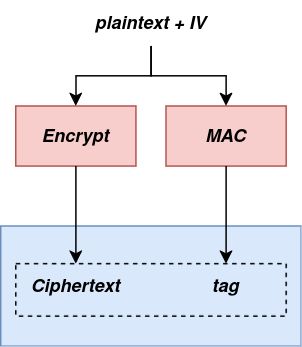
\includegraphics[width=0.75\textwidth]{img/enc_and_mac.png}
            
            In questo caso viene cifrato il testo in chiaro e composto il MAC in maniera parallela e poi vengono concatenati i risultati. Non ho alcuna garanzia che garantisca la confidenzialità del messaggio.

        \end{minipage}
        \begin{minipage}[c]{0.30\textwidth}
            \centering
            \textbf{\textit{MAC-then-Encrypt}} \\
            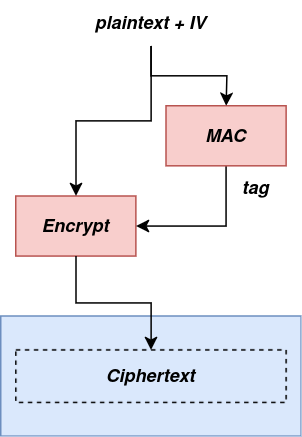
\includegraphics[width=0.75\textwidth]{img/mac_then_enc.png}

            Prima calcola il \textit{tag} e poi cifra la concateazione tra \textit{tag} e \textit{plaintext}.

        \end{minipage}
        \begin{minipage}[c]{0.30\textwidth}
            \centering
            \textbf{\textit{Encrypt-then-MAC}} \\
            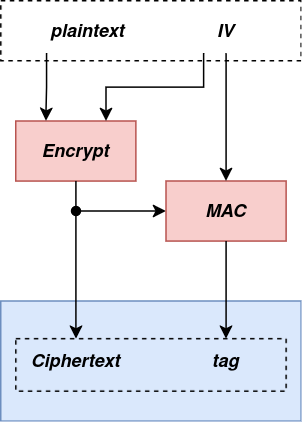
\includegraphics[width=0.75\textwidth]{img/enc_then_mac.png}

            Prima si calcola il crittogramma che poi verrà utilizzato per generare il \textit{tag}, concatenando in seguito il risultato. Il MAC è calcolato sul testo cifrato quindi non è possibile informazioni aggiuntive

        \end{minipage}
    \par}

    Considerando tutti e tre le combinazioni degli schema l'unica che garantisce il rispetto dei requisiti di sicurezza anche senza considerare le primitive sottostantei è l'\textbf{\textit{encrypt-then-MAC}}.
    \begin{enumerate}[nosep]
        \item la funzione \textbf{MAC} deve autenticare non solo il testo cifrato, ma anche l'IV.
        \item lo schema di crittografia e la funzione di MAC devono utilizzare due tipologie di \textbf{chiavi differenti}.
        \item nella fase di \textit{decryption} il \textbf{tag} deve essere verificato \textbf{prima} di iniziare la decifratura in quanto un'attaccante potrebbe mettere in pratica un \textbf{\textit{timing attack}}, ovvero ottenere informazioni dal tempo di esecuzione di una certa funzione.
    \end{enumerate}
    Un'altra cosa fondamentale è che le funzioni crittografiche (\textit{encryption} e \textit{decryption}) devono essere \textbf{\textit{time-constant}}
\end{flushleft}

\newpage

\begin{flushleft}
    \textcolor{red}{\textbf{\textit{Authenticated Encryption with Associated Data - AEAD}}}
    \begin{lstlisting}
    key = keygen([size])
    cipher = encrypt(key, nonce/iv, a, plain)
    plain = decrypt(key, nonce/iv, a, cipher)
    \end{lstlisting}
    \vspace*{-\baselineskip}
    I \textbf{dati associati} non sono cifrati né inclusi nel crittogramma (principalmente per vincoli definiti dal contesto in cui sono), ma l'autenticità è invece vincolata anche a quell'informazione. In questo modo l'operazione di decifratura verificherà che gli \textit{associated data} siano gli stessi dell'\textit{encryption}, in caso contrario, \textbf{fallirà} riuscendo a garantire:
    \begin{itemize}[nosep]
        \item confidenzialità, autenticità e integrità del \textit{plaintext}.
        \item autenticità e integrità dei dati associati.
    \end{itemize}
    Aggiungono \textit{overhead} sia a livello computazine che di \textit{storage}.
\end{flushleft}

\section{IND-CCA1 Encryption Schemes \\ \small{length-preserving scheme for disk encryption}}

\begin{flushleft}
    Non è possibile garantire forte autenticità (CCA2) senza adottare l'uso di MAC, ma in questo modo uno schema \textit{CCA2 secure} introdurrà dell'\textit{space overhead} rispetto a schemi non autenticati. In certi scenari è preferibile - se non richiesto - che il testo cifrato abbia la \textbf{stessa dimensione} del \textit{plaintext}, molti di questi scenari sono i \textbf{\textit{disk (sector) encryption}}. In questi scenari la migliore sicurezza che riusciamo a garantire è \textbf{IND-CCA1}.

    \smallskip

    Per come si è descritto lo scenario un \textit{stream cipher} - che per definizione è completamente \textbf{malleabile} - è la peggior progettazione possibile in quanto non possiamo autenticare (in quanto introducerebbe un \textit{overhead}), è quindi guidata la scelta verso i \textit{block cipher} - storicamente è sempre stato preferito il \textit{mode of operations} \textbf{CBC}. I problemi di \textbf{CBC} legati ad attacchi attivi sono:
    \begin{itemize}[nosep]
        \item molto vulnerabili contro la \textbf{manipolazione dell'\textit{IV}}.
        \item molto vulnerabili contro attacchi del tipo \textbf{\textit{ciphertext substitutions}} (es. \textit{efail}).
        \item il \textit{padding} può aiutare l'attaccante.
        \item ``\textit{functional issue}'': i blocchi sono \textbf{interdipendenti}.
    \end{itemize}

    \smallskip

    Per la cifratura del disco ci sono alcuni requisiti che vanno rispettati, tra cui: la lunghezza del testo cifrato deve essere uguale al testo in chiaro (nessun \textit{IV} o \textit{nonce} e nessun \textit{tag}), livello di sicurezza contro \textbf{attacchi CCA1} (è impossibile per l'attaccante avere un riscontro di cosa è stato modificate - scenario non adattivo) e ultimo, ma non per importanza è che devono essere veloci. Da questo possiamo andare a definire cosa alcune intuizioni di progettazione:
    \begin{itemize}[nosep]
        \item la crittografia deve essere a \textbf{blocchi}.
        \item i blocchi devono essere \textbf{indipendenti} uno dall'altro, ma comunque non malleabili (\textbf{no CTR}) e random (\textbf{no ECB}).
        \item la randomicità non deve però introdurre problematiche di malleabilità e deve essere indipendente da ogni blocco (\textbf{no CBC-IV} con effetto a valanga).
        \item è possibile utilizzare i \textbf{\textit{sector number}} - anche noti come \textbf{\textit{tweaks}} - al posto del nonce.
    \end{itemize}
    Ricordiamoci che la garanzia di sicurezza richiesta da questo scenario è \textbf{\textit{CCA1 secure}}, senza però essere autenticata il che comporta non riuscire a rilevare modifiche a livello crittografico. È possibile però incorporare una struttura aggiuntiva a livello di codifica per avere un'autenticazione forte - il \textit{filesystem} può garantire l'integrità ad esempio con un \textit{checksum}.
\end{flushleft}

\begin{flushleft}
    \textcolor{red}{\textbf{\textit{XTS operation mode}}}: è stata standardizzata nel 2007 dalla \textit{IEEE} e nel 2010 dal \textit{NIST}, garantisce che una modifica nel \textit{ciphertext} causi una modifica random nel \textit{plaintext}, queste modifiche sono propagate unicamente in quel blocco
    
    \smallskip

    \textcolor{red}{\textbf{\textit{Adiantum}}} encryption: molto veloce in \textit{software}, consigliata nel momento in cui non è presente un acceleratore hardware per AES. È utilizzato come default per versioni di Android $\geq 10$ e per \textit{lower-end device} senza supporto AES hardware (negli altri casi viene preferito \textbf{AES-XTS}). Può utilizzare diversi \textit{block cipher} come primitive (NH hash, ChaCha12, Poly1305, AES) ed è stata resa disponibile nel kernel main-line di linux dalla versione 5.0.

    \smallskip

    \textcolor{red}{\textbf{\textit{HCTR2}}}: necessita accelerazione hardware per AES, è stato integrato nel kernel di linux nel Maggio 2022.

    \textbf{Adiantum} e \textbf{HCTR2} sono \textbf{CCA1 \textit{secure \underline{wide}-block encryption}}.

    {\centering
        \begin{minipage}[t]{0.45\textwidth}
            \textbf{\textit{Narrow Block Encrypt}} \\
            \textbf{XTS} è \textbf{\textit{IND-CCA1 narrow block encryption}} e lavora con blocchi di lunghezza pari alla \textit{block size} (128bit per \textbf{AES}). Nel caso di compromissione o tentata manipolazione di un bit, questa verrà propagata unicamente all'interno del blocco corrente.
        \end{minipage}
        \hfill
        \begin{minipage}[t]{0.5\textwidth}
            \textbf{\textit{Wide Block Encrypt}} \\
            \textbf{Adiantum} e \textbf{HCTR2} sono invece \textbf{\textit{IND-CCA1 wide block encryption}} ovvero lo schema accetta un'altro parametro: la \textbf{\textit{block size}}, riesce a ricostruire uno algoritmo partendo da \textit{block cipher} con \textit{block size} più piccola (esistono limitazini legate alla sicurezza). Viene modellato come una \textbf{\textit{Super Pseudo Random Permutation - SPRP}}. Nel caso di compomissione o tentata manipolazione di un bit, questa verrà propagata anche nei blocchi adiacenti aiutando ad identificarle in maniera più precisa.
        \end{minipage}
    \par}
    Un \textbf{\textit{disk sector}} è di 4096 bytes, se noi andiamo ad impostare la dimensione del blocco in un algoritmo \textbf{\textit{wide block encryption}} questo sarà molto più ottimizzato.
\end{flushleft}

\section{XTS Operation Mode \\ \small{CCA1 narrow block encryption}}

\begin{flushleft}
    \textcolor{red}{\textbf{\textit{X}}}\textbf{\textit{EX}}-based \textcolor{red}{\textbf{\textit{T}}}\textbf{\textit{weaked-codebook}} mode with \textbf{\textit{ciphertext }}\textcolor{red}{\textbf{\textit{S}}}\textbf{\textit{tealing}}
    \begin{itemize}[nosep]
        \item \textcolor{red}{\textbf{\textit{Tweakable Block Cipher}}}: può essere considerata una \textbf{primitiva crittografica} che estende un classico \textbf{block cipher} con un input aggiuntivo: il \textbf{\textit{tweak}} che è simile al \textit{nonce} in modello che è resistente al \textit{nonce-reuse}: pubblico, univoco (la duplicazione non rompe la cifratura) e non ha requisiti di randomicità. È applicato ad un singolo blocco.

        {\centering
            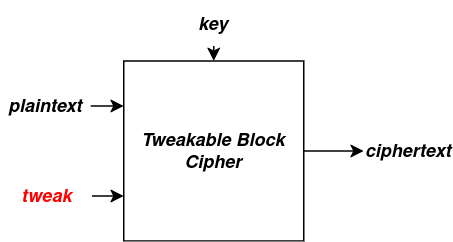
\includegraphics[width=0.45\textwidth]{img/tweak_bd.png}
        \par}

        \item \textcolor{red}{\textbf{\textit{Xor Encrypt Xor - XEX}}} è una progettazione standard per costruire un \textit{tweakable cipher} basandosi su un \textit{block cipher} standard, garantendo \textbf{\textit{length-preserving}} accetta in input dati che abbiano dimensione multipla della \textit{block size}. \textbf{XEX} necessita di \textbf{due chiavi distinte}, che possono essere derivate o estese dalla stessa dal \textit{layer} sopra.

        \begin{figure}[h]
            \centering
            \begin{minipage}[c]{0.45\textwidth}
                \centering
                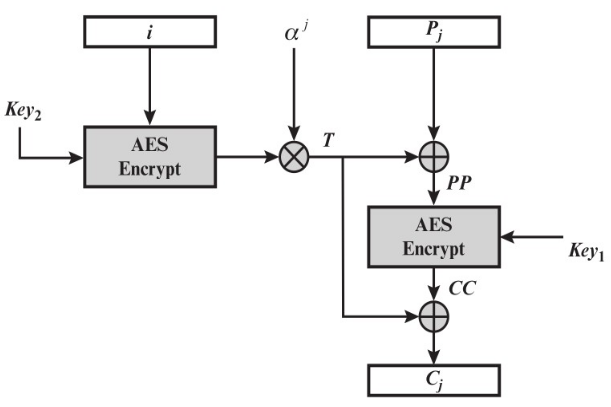
\includegraphics[width=\textwidth]{img/xex_enc.png}
                \caption{XEX Encryption}
            \end{minipage}
            \hfill
            \begin{minipage}[c]{0.45\textwidth}
                \centering
                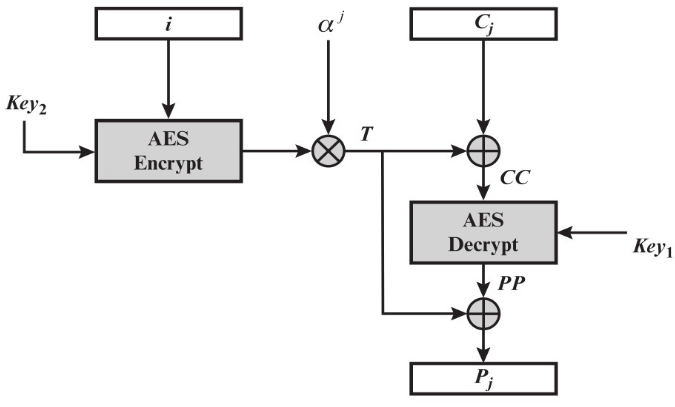
\includegraphics[width=\textwidth]{img/xex_dec.png}
                \caption{XEX Decryption}
            \end{minipage}
        \end{figure}
        
        \item \textcolor{red}{\textbf{\textit{Ciphertext Stealing - CTS}}}: è una tecnica utilizzata per supportare dati di lunghezza variabile negli schemi di cifratura a blocchi, tuttavia introduce un stretta dipendenza tra gli ultimi due blocchi, a volte è stata anche utilizzare per mitigare gli attacchi legati al \textit{padding oracle}, oggi si preferisce la cifratura autenticata.

        \begin{figure}[h]
            \centering
            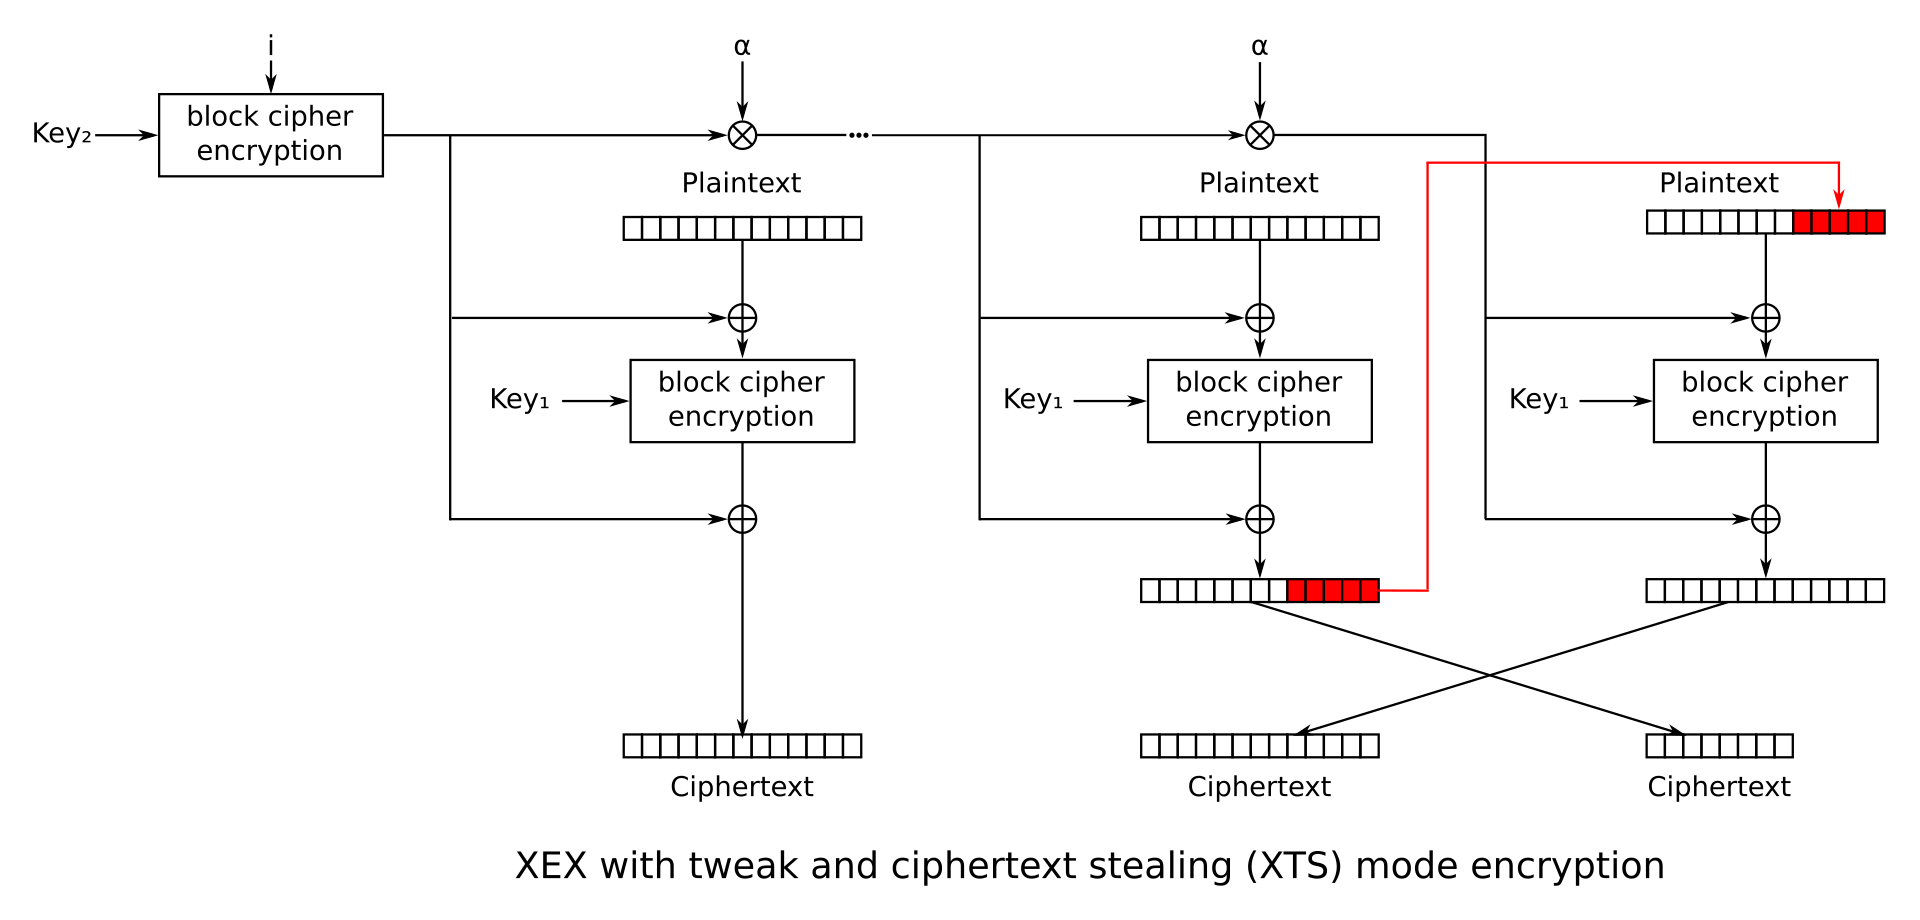
\includegraphics[width=\textwidth]{img/xts.png}
            \caption{XTS Encryption}
        \end{figure}
    \end{itemize}
\end{flushleft}

\section{Wide Block Encryption}
\begin{flushleft}
    Un blocco \textbf{\textit{wide encryption}} è modellato per la cifratura di \textit{disk sector} ed è rappresentabile come un \textbf{\textit{Super Pseudo Random Permutation}} che accetta come parametri:
    \begin{itemize}[nosep]
        \item un \textbf{\textit{tweak}} per supportare la randomizzazione basata sulla locazione dell'informazione.
        \item una \textbf{\textit{block size}} che regola la quantità di dati che è contenuta nella permutazione.
    \end{itemize}
    È basato su un \textit{block cipher} con una dimensione ridotta e fissa.

    \begin{figure}[h]
        \centering
        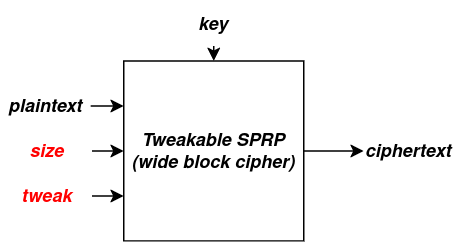
\includegraphics[width=0.45\textwidth]{img/wide_block.png}
    \end{figure}
\end{flushleft}
\chapter{Randomness}
\begin{flushleft}
    I protocolli di crittografia sono spesso basati su \textbf{generatori di dati random}, ad esempio per la generazione delle \textbf{chiavi} o dell'\textbf{IV}. È importante differenziare un valore random con un valore \textbf{crittograficamente randomico} ovvero dati \textbf{impredicibili} che possono essere campionati da una distribuzione uniforme o coinvolgere altre tipologie di distribuzione - ad esempio quella Gaussiana. \\
    Molti eventi del mondo reale sono noti - nella fisica - come governati  da:
    \begin{itemize}[nosep]
        \item eventi probabilistici che sono ``realmente'' casuali o imprevedibili, ad esempio quelli studiati dalla fisica quantistica.
        \item comportamenti deterministici che sono molto difficili da prevedere in quanti gli output sono molto sensibili anche a variazioni molto piccole degli input, normalmente studiati nella teoria del caos.
    \end{itemize}

    \smallskip

    \textcolor{red}{\textbf{Entropia}}: in ambito crittografico rappresenta l'imprevedibilità di un'informazione, maggiore è l'entropia, più è difficile per un attaccante indovinare o ricostruire quel dato. Ad esempio consideriamo una chiave a 128bit generata partendo da una scelta casuale di un solo bit attraverso un algoritmo deterministico, a quel punto avremo che la lunghezza della chiave sarà 128bit, ma i suoi bit di entropia sarà soltanto uno e questo fatto la rende facilmente attaccabile. \\
    Normalmente in crittografia si richiede che la chiave abbia $n$ bit di \textbf{entropia}, ovvero il nostro spazio delle chiavi sarà formato da $2^n$ tutti \textbf{equiprobabili}. Queste congettura, tuttavia, non valgono per \textbf{password} o \textbf{PIN}.

    \smallskip

    Consideriamo \textbf{chiavi crittografiche segrete uniformemente casuali} su stringhe binarie: in questo caso la lunghezza in bit è pari all'entropia della chiave. Nel caso di \textbf{PIN} avremo una sequenza di $n$ numeri, possiamo calcolare la probabilita che esca un determinato numero: $\log_2(10^n)$ - ad esempio per $n = 4$ avremo che i bit di entropia saranno $\log_2(10^4) \simeq 13.28$bit. Invece, per una \textbf{password}, dipende dall'alfabeto scelto ($n$) - quindi la sua cardinalità - e dalla lunghezza della password ($N$), il calcolo dei bit di entropia sarà: $N \times \log_2(10^n)$. Nel caso di \textbf{password} il reale livello di sicurezza è molto più basso in quanto il campionamento dei simboli non è sempre uniforme all'interno del loro dominio o indipendentemente l'uno dall'altro. Infatti difficilmente la mente umana è capace di ricordarsi dati completamente random e quindi la sicurezza di una password di dimensione $N$ è molto inferiore alla precendente stima.

    \smallskip

    Considerando applicativi su cui è necessario far girare algoritmi di crittografia, e considerando che tali applicativi sono software, per ottenere un dato random ``buono'' non possiamo affidarci ad un computer in quanto sono intrinsecamente \textbf{deterministici} e \textbf{predicibili} è quindi necessario fare affidamente su \textbf{fonti esterne} che sono associate a dati intrinsecamente randomici o eventi fisici impredicibili (camere, input dell'utente, \textit{interrupt hardware}). Esisto degli hardware dedicati, chiamati: \textbf{\textit{True Random Number Generator - TRNG}} che venono alimentati da eventi fisici (\textit{thermal noise}) che vengono quindi utilizzati come fonti esterne di bit random (molto utili per server e sistemi embedded), queste sorgenti esterne vengono spesso identificate come \textbf{\textit{noise source}}
    
    \smallskip

    Le \textbf{sorgenti di entropia} vengono prima processate dal sistema operativo prima di essere rese disponibili ad altri servizi. Questo permette di ottenere fonti di entropia miste:
    \begin{itemize}[nosep]
        \item aumento di ``fiducia'' nella qualità dei dati casuali.
        \item mitigare potenziali rischi di attacchi alle fonti.
        \item ridurre i rischi relativi alle fonti di \textbf{backdoor}
    \end{itemize}
    Inoltre permette anche di espandere i ``veri'' dati casuali per aumentare la disponibilità di dati ad alta entropia.

    \begin{figure}[h]
        \centering
        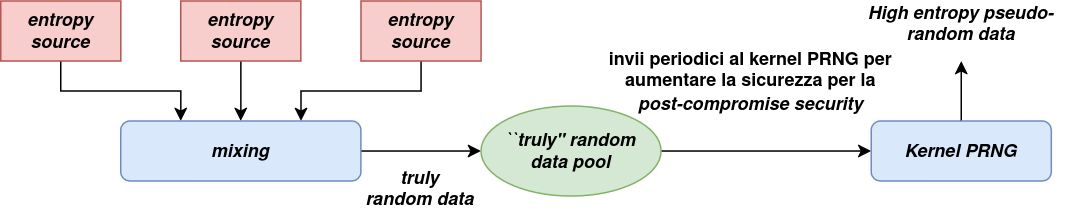
\includegraphics[width=0.75\textwidth]{img/prng_pool.png}
    \end{figure}

    Il lavoro del \textbf{\textit{Kernel PRNG}} è simile a quello di uno \textit{stream cipher} ma il suo schematico è leggermente differente in quanto vi è una modellazione dell'avversario diversa. Che permette di aumentare la sicurezza attraverso lo sviuppo di mitigazioni contro a \textbf{compromissioni non permanenti}:
    \begin{itemize}[nosep]
        \item \textbf{\textit{forward secrecy}}: se l'avversario compromette il sistema in un istante di tempo $t_i$ non dovrà riuscire ad ottenere informazioni su istanti di tempo $t_k$ con $k < i$, per ottenere questa garanzia si possono utilizzare delle funzioni \textbf{\textit{one-way}} - ad esempio le \textit{hash function}.
        \item \textbf{\textit{post-compromise security}}: è duale alla \textit{forward secrecy} ovvero che se l'avversario compromette il sistema in un istante $t_i$ non dovrà riuscire ad ottenere stati futuri in maniera deterministica.
    \end{itemize}
    Queste due proprietà (\textbf{\textit{Security Guarantees}}) vanno a descrivere un attaccante che non deve essere capace di creare persistenza nel sistema.

    \smallskip

    \textbf{\textit{Kernel vs. User space}}, in passato molte librerie crittografiche non si fidavano della routine del sistema operativo per generare numeri casuali sicuri, infatti si credeva che il \textbf{kernel} avesse una \textbf{PRNG} debole venne quindi adottata una soluzione, ovvero le librerie crittografiche \textbf{implementavano} un priorio \textit{PRNG custom} in \textbf{\textit{user space}} - chiamato anche \textbf{\textit{userland PRNG}}, ma veniva spesso sbagliata l'impementazione e questi dati avere un entropia molto bassa. Un esempio famoso fu nel 2008 che debian, dopo una modifica al codice sorgente rese prevedibile la generazione della chiave private ssh. Oggigiorno ci si affida maggiormente al sistema operativo e alle API per la generazione di valori randomici.
    
    \smallskip

    Un altro problema molto importante era il \textbf{\textit{reesiding at fork}} infatti se non specificato, nel momento in cui veniva eseguita una \textbf{fork} e successivamente \textit{spawnato} un processo figlio se non veniva aggiornato il pool di entropia, sia il padre che il/i figli avrebbero generato la stessa sequenza di valore \textit{pseudo-random}.

    \smallskip

    \textbf{\textit{Virtual Machine Cloning}}: clonare una macchina virtuale poteva causare problemi al \textit{kernel PRNG} simili all'utilizzo di una \textbf{fork} questo comportava:
    \begin{itemize}[nosep]
        \item multi-VMs accese nello stesso istante generavano gli stessi pseudo-random data.
        \item la soluzione fu quella di re-inizializzare il pool durante l'avvio della VMs
    \end{itemize}

    \smallskip

    \textbf{\textit{Low entropy in early boot phases and embedded devices}} nelle fasi iniziali di boot, soprattuto nei dispositivi embedded, il pool potrebbe essere molto basso, se non inesistente questo comportava l'arresto o la generazione di pseudo-random deboli a seconda della strategia adottata - bloccante o attesa - la soluzione fu quella di adottare una \textbf{\textit{TRNG Hardware}}
\end{flushleft}
\chapter{Derived Schema of Symmetric Crypto}

\section{SHA3 Derived Schemes}
\begin{flushleft}

    Abbiamo detto che una funzione hash ritorna come output una quantità fissa di bytes. Se quindi ci dovesse essere la necessità di avere \textbf{meno dati}, allora ``basterebbe'' \textbf{troncare} il \textbf{\textit{digest}}, nel caso opposto invece possiamo ri-progettare un algoritmo simile a \textbf{CTR} e invocarlo più volte, il che, però, porterebbe molto più sforzo da parte degli sviluppatori e rischierebbe di introdurre delle vulnerabilità nel codice.
    
    \smallskip

    È stato quindi introdotto il \textbf{\textit{eXtendible Output Function - XOF}} ovvero una \textbf{\textit{variable-length hash funciton}}.

    \smallskip

    \textcolor{red}{\textbf{\textit{cSHAKE}}}: è una variante di SHA3 e accetta i seguenti input addizionali:
    \begin{enumerate}[nosep]
        \item \textbf{\textit{output length}}: definisce la dimensione del digest.
        \item \textbf{\textit{custom string}}: specializza l'esecuzione della funzione \textit{hash} per un certo \textbf{contesto}. È molto utile per \textbf{\textit{domain (contest) separation}}.
    \end{enumerate}

    \begin{figure}[h]
        \centering
        \begin{minipage}[c]{0.45\textwidth}
            \textbf{cSHAKE128} ha 128bit di sicurezza ed è una variante di SHA3-256.
        \end{minipage}
        \hfill
        \begin{minipage}[c]{0.45\textwidth}
            \textbf{cSHAKE256} ha 256bit di sicurezza ed è una variante di SHA3-512.
        \end{minipage}
    \end{figure}

    \smallskip

    \textcolor{red}{\textbf{\textit{TupleHash}}}: è una funzione \textit{hash} ha delle interfacce con un astrazione \textit{high-level}, infatti permette di accettare una \textbf{lista di valori} e una \textbf{\textit{custom string}} come input. È un \textit{wrap} di \textbf{cSHAKE} che permette di supportare delle liste come valore di input, alle quali viene prima applicata una codifica in modo non ambiguo assegnando ad ogni elemento un'unica sequenza di bit - bitstring - poi verrà passata a cSHAKE come input. La \textit{custom string} ha un valore di default al quele viene concatenato quello dell'utente: \textit{TupleHash}. È utilizzata per evitare ambiguità di concatenazione. È deterministica e strutturate, utile in contesti crittografici dove serve un hash sicura su strutture dati complesse.

    \smallskip

    \textcolor{red}{\textbf{\textit{ParallelHash}}}: è progettato per per sfruttare ambienti paralleli (multi-core, GPU, ecc.) allo scopo di accelerare il calcolo dell'hash su grandi quantità di dati.
    \begin{enumerate}[nosep]
        \item i dati vengono suddivisi in blocchi.
        \item per ogni blocco viene calcolato il \textit{digest} in parallelo.
        \item i \textit{digest} dei vari blocchi (\textbf{\textit{digest parziali}}) vengono poi combinati per calcolare un \textit{digest} finale sugli output precedenti, ottenendo il digest complessivo del messaggio.
    \end{enumerate}
    Questo approccio ricorda un \textbf{\textit{Merkle Hash Tree - MHT}} dove le foglie sono gli hash dei blocchi e il nodo radice è l'hash finale ottenuto dall'unione degli hash sottostanti. \\ 
    \textbf{\textit{N.B.}} esistono funzioni di hash - ad esempio \textbf{Blake2} - che hanno meccanismi interni che la rendono automaticamente parallelizzabili anche senza un architettura come quella di ParallelHash.

    \smallskip

    \textcolor{red}{\textbf{\textit{MAC for SHA3}}}: \textbf{SHA3} è stato progettato e sviluppato per evitare \textbf{\textit{length extesion attack}} è quindi possibile non utilizzare l'\textbf{HMAC} basato su SHA3, in quanto ci sarebbe dell'\textit{overhead} inutile, ma sarebbe possibile avere un MAC che si basa su SHA3 come:

    {\centering
        \textbf{tag} $\leftarrow$ \textcolor{red}{\textbf{SHA3(k || message)}}
    \par}

    Bisogna solo fare attenzione a non utilizzare questo metodo con funzioni di hash che utilizzano come primitiva la costruzione \textbf{Merkle-Damgard} - per SHA2 utilizzare HMAC.

    \smallskip

    \textcolor{red}{\textbf{\textit{KMAC}}}: è un \textbf{MAC} a dimensione variabile che si basa su \textbf{cSHAKE}. Come input \textbf{KMAC} richiede:
    \begin{enumerate}[nosep]
        \item una \textbf{chiave} segreta $k$.
        \item un \textbf{messaggio} $m$.
        \item una \textbf{\textit{custom string}} che verrà concatenato al valore di default \textit{KMAC}.
        \item una \textbf{lunghezza} desiderata dell'output.
    \end{enumerate}
    Vengono combinati, in maniera sicura, la chiave, il messaggio e la \textit{custom string}, il tutto viene passato in input a cSHAKE che ne calcola il \textbf{tag}.

    \begin{figure}[h]
        \centering
        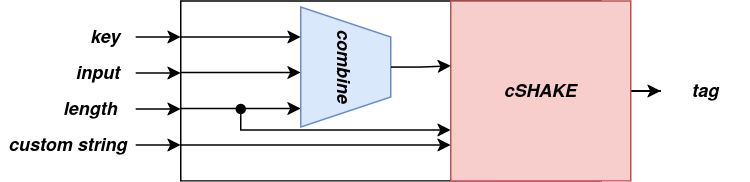
\includegraphics[width=0.75\textwidth]{img/kmac.png}
    \end{figure}
\end{flushleft}

\newpage

\section{Key Derivation Function}

\begin{flushleft}
    Molti schemi crittografici e protocolli spesso richiedono almeno due chiavi segrete non correlate, ma di contro si cerca di dover gestire un'unica chiave durante le procedure di \textit{key management} e di \textit{key distribution}.

    \smallskip

    Le \textbf{\textit{KDF}} sono funzioni che permetto di generare più \textit{pseudo-random keys} partendo da una singola chiave. Le \textbf{KDF} sono simili a delle \textbf{PRF}, infatti, prendono in input una singola stringa segreta e in maniera \textbf{deterministica} in output verrà generata una sequenza più lunga di dati pseudo-random che possono essere utilizzate come chiavi indipendenti e multiple. A differenza dei \textbf{PRF}, però, la \textbf{KDF} è progettata per generare una sequenza più corta e in più possono supportare altre funzionalità - ad esempio \textbf{\textit{input string}}, \textbf{\textit{explicit salting}} e lo \textbf{\textit{scoping}}. \\
    È possibile re-implementare una \textbf{KDF} utilizzando come primitive \textit{block cipher}, \textit{stream cipher}, MAC o \textit{hash function}. Esistono, però, delle \textbf{KDF} stardandizzate dal NIST, la più popolare è chiamata \textbf{HKDF} e si basa su un \textbf{HMAC}.

    \smallskip

    Un'implementazione di alto livello di una \textbf{KDF} ha due funzioni interne:
    \begin{enumerate}[nosep]
        \item \textcolor{red}{\textbf{\textit{extraction}}}: che dato una \textit{secret string} - possibilmente \textbf{non uniforme} e con un \textbf{alto livello di entropia} (comparabile con il \textit{security level}) - genera \textbf{una} chiave segreta (pseudo-random) uniforme.
        \item \textcolor{blue}{\textbf{\textit{expansion}}}: data una \textit{secret key} uniforme genera una chiave \textbf{pseudorandom} più lunga - ad esempio generare una chiave da un'altra per \textit{key scoping} o \textit{key rotation}
    \end{enumerate}

    \begin{figure}[h]
        \centering
        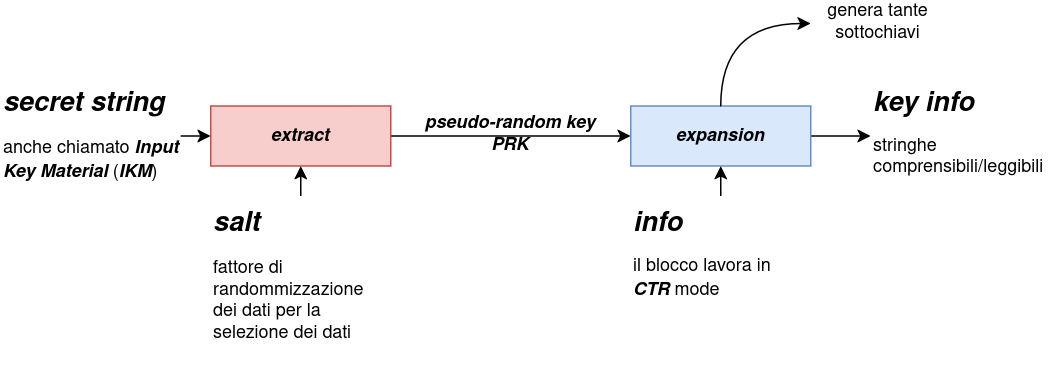
\includegraphics[width=\textwidth]{img/kdf.png}
    \end{figure}

    Una \textbf{KDF} è un metodo sicuro per derivare una chiave segreta anche se l'input è una string non uniforme (uniforme = alta entropia), ma l'input deve avere alta entropia e, ad esempio, una password per definizione - segreto che può essere ricordato da un umano - raramente ha abbastanza entropia $\rightarrow$ \textbf{\textit{Password-Based Key Derivation}} anche note come \textbf{\textit{Password Hashing}}. Nel caso in cui si abbia già un segreto random binario possiamo \textit{bypassare} il blocco di \textbf{\textit{extract}} e passare subito all'\textbf{\textit{expansion}}. Una \textbf{KDF} può dare funzionalità aggiuntive tra cui: aggiungere \textbf{randomicità} e aggiungere \textit{scoping information} (ad esempio per fare \textit{domain separation}).

    \smallskip

    Gli input di una \textbf{KDF} sono:
    \begin{itemize}[nosep]
        \item l'\textbf{algoritmo}: la funzione di hash interna (SHA256).
        \item \textbf{\textit{string}}: è la stringa segreta (con alta entropia).
        \item \textbf{\textit{length}}: lunghezza desiderata per la chiave derivata - simile all'input della dimensione per \textbf{XOF} e \textbf{KMAC}.
        \item \textbf{\textit{info}}: è una stringa che rappresenta il contesto per la separazione dei domini.
        \item \textbf{\textit{salt}}: è una stringa, è opzionale, se viene utilizzata normalmente è una stringa randomica con lunghezza compatibile con la dimensione dell'algoritmo di hash utilizzato per l'\textbf{HMAC}
    \end{itemize}
    L'output è una \textbf{chiave pseudorandom} di dimensione \textbf{\textit{length}}.
\end{flushleft}

\chapter{Authenticated Protocol pt. 1}

\begin{flushleft}
    I moderni sistemi informativi devono implementare dei controlli per l'\textbf{identificazione}, l'\textbf{autenticazione} e \textbf{autorizzazione} per gli utenti:
    \begin{itemize}[nosep]
        \item \textbf{identificazione}: bisogna garantire univocità nel riconoscimento di un utente.
        \item \textbf{autenticazione}: permette di prevenire che un'attaccante impersonifichi un attore legico.
        \item \textbf{autorizzazione}: determina a quali risorse un utente autenticato può accedere.
    \end{itemize}

    \textcolor{red}{\textbf{\textit{AutN} - Autenticazione}}: è il processo per determinare se un utente ha o meno \textbf{accesso} al \textbf{sistema}.
    
    \smallskip

    \textcolor{red}{\textbf{\textit{AutZ} - Autorizzazione}}: è il processo per regolare a quali risorse un utente autenticato è autorizzato ad accedere - la tipologia di regole che vengono applicate dipendono dal \textit{access model control} adottato.
\end{flushleft}

\begin{boxA}
    \textcolor{orange}{\textbf{Esempio - \textit{Authentication in WebApp}}}

    \begin{center}
        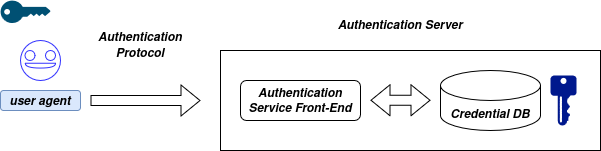
\includegraphics[width=0.75\textwidth]{img/web_app_auth.png}
    \end{center}

    È possibile estendere la complessità dell'architettura in modo da permettere \textbf{\textit{Single Sign On (SSO)}}, \textbf{\textit{Identity Federation (OpenID)}}, \textbf{\textit{Authorization delegation (OAuth2)}}, ma tutti questi hanno come blocco base (primitiva) l'autenticazione dell'utente.
\end{boxA}

\begin{flushleft}
    La procedura di \textbf{autenticazione} si basa su \textbf{fattori di autenticazione} (\textbf{\textit{authentication factor}}), ovvero dei metodi che utilizza un utente per dimostrare la sua identità, vengono anche chiamate \textbf{credenziali}. Ci sono diverse tipologie di fattori di autenticazione:
    \begin{itemize}[nosep]
        \item qualcosa \textbf{posseduto} dall'utente, ad esempio: \textbf{PIV - \textit{Personal Identifty Verification card}} o \textbf{U2F - \textit{Universal 2nd Factor}}.
        \item qualcosa \textbf{conosciuto} dall'utente, ad esempio una \textbf{password} o un \textbf{PIN}.
        \item Qualcosa che può essere eseguito dall'utente, tipologie di gesti.
    \end{itemize}
    Una procedura di autenticazione può richiedere ad un utente di fornire uno o più fattori di autenticazione - al giorno d'oggi è consigliato avere la \textbf{\textit{two-factor authentication}}.

    \medskip

    \textbf{Classi di Attacco}:
    \begin{enumerate}[nosep]
        \item attacchi \textit{client-side} (attacchi all'utente o al dispositivo dello stesso): possono essere ``\textbf{\textit{on-site}}'' ovvero un attacco allo \textbf{\textit{user-agent}} oppure attacchi ``\textbf{\textit{in motion}}'' quindi un attacco al canale di comunicazione, come ad esempio \textbf{\textit{snooping}}, \textbf{\textit{man-in-the-middle}} e \textbf{\textit{phishing}}
        \item attacchi \textit{server-side} che possono essere divise a loro volta in: \textbf{sfruttamento di \textit{weak credentials}} presenti nel servizio di autenticazione oppure \textbf{accesso alle credenziali del DB} anche noto come \textbf{\textit{data breach}}
    \end{enumerate}
\end{flushleft}

\section{Types of AuthN Protocol}

\begin{boxA}
    \textcolor{red}{\textbf{\textit{CAPTCHA - ``Turing Test''}}} \\
    Definiamo il concetto di utente: vogliamo differenziare gli ``umani'' da computer, anche detti \textbf{bot}. Vorremmo che l'autenticazione fosse riservata a persone, in modo da escludere bot che potrebbero essere degli \textit{exploit} eseguiti da un attaccante per automatizzare, ad esempio, il \textit{brute force} delle password. Il \textbf{CAPTCHA} è una procedura che ne ingloba altre, normalmente definite difficili o impossibili per un computer, per escludere che un utente sia un bot.

    \smallskip

    Un tipo particolare di CAPTCHA viene detto \textbf{reCAPTCHA} e si basa su degli input presi dal mondo reale. Spesso vengono fornite dalle aziende in maniera ``\textit{as-a-service}''
\end{boxA}

\begin{flushleft}
    \textcolor{red}{\textbf{\textit{Bearer Token}}} - \textit{basic authentication} \\
    Il protocollo di autenticazione più semplice è la dimostrazione di conoscere un segreto, che deve essere inviato al servizio ``\textit{as-is}'', ma deve essere ovviamente fatto attraverso un canale di comunicazione sicuro, nel caso opposto un avversario sarebbe capace di leggerlo. Il \textit{bearer token} può essere implementato in vari modi, ad esempio: password, \textit{API key}, \textbf{JWT}. Lo svantaggio maggiore è che se l'attaccante è capace di ottenere il segreto in transito è capace di \textbf{impersonificare permanentemente} l'utente - almeno finché la credenziale non verrà revocata.
\end{flushleft}

\begin{flushleft}
    \textcolor{red}{\textbf{\textit{One-time credentials}}} \\
    Permette di mitigare il danno in caso di accesso alla password sul canale di comunicazione tramite l'invio di \textbf{diverse \textit{authentication information} per ogni autenticazione}. Dopo ogni autenticazione il server \textbf{invalida} la credenziale utilizzata. Il \textcolor{olive}{\textbf{vantaggio}} è che anche violando il canale trasmissivo il danno è limitato, lo \textcolor{red}{\textbf{svantaggio}} è che il \textit{client} e \textit{server} devono riservare dello spazio propozionale al numero di procedure di autenticazione.
    
    \smallskip

    \textbf{\textit{Backup OTP codes}}: credenziali monouso pregenerate da mantenere offline in maniera sicura.
\end{flushleft}

\begin{flushleft}
    \textcolor{red}{\textbf{\textit{Challenge-Response}}} \\
    I protocolli del tipo \textit{challenge-response} consentono agli utenti di calcolare un valore in relazione ad una \textit{challenge} utilizzando le proprie credenziali utente. Le credenziali non vengono mai inviate attraverso il canale trasmissivo, e la sfida è monodirezionale per evitare attacchi del tipo \textbf{\textit{reply}}. Le credenziali potrebero non essere note all'utente ma solamente controllate. Alcuni esempi possono essere \textit{challenge} basate sul \textbf{tempo} (preso nell'istante di tempo iniziale della comunicazione, con una certa \textbf{tolleranza}) - nei server web è sempre presente (\textbf{NTP}) a differenza degli apparati embedded.

    \smallskip

    I protocolli \textit{challenge-response} possono essere implementati sia con crittografia \textbf{simmetrica} che tramite crittografia \textbf{asimmetrica}. In un caso la chiave di autenticazione è uguale a quella di verifica, nell'altro divergono.
\end{flushleft}

\begin{flushleft}
    \textcolor{red}{\textbf{\textit{Credential Ddatabases}}}: i database richiesti per permettere protocolli di autenticazione possono includere diverse tipologie di informazioni in relazione al tipo di protocollo utilizzato.
    \begin{itemize}[nosep]
        \item \textbf{\textit{bearer token}} (o informazioni derivate)
        \item \textbf{\textit{public keys}} (crittografia asimmetrica)
        \item \textbf{\textit{secret keys}}
        \item altri \textbf{metadati} o materiale crittografico
    \end{itemize}
    Il \textbf{database delle credenziali} è normalmente \textbf{statico} - a differenza \textcolor{red}{\textbf{\textit{dynamic credential database}}} che permette di aumentare la \textbf{resilienza} delle credenziali salvate modificandolo - il che implica che non varia durante tutta la procedura di autenticazione.
\end{flushleft}

\newpage

\section{OTP, OATH OTP}

\begin{flushleft}
    Andiamo ad analizzare i protocolli \textcolor{red}{\textbf{\textit{Challenge-Response based on Symmetric Cryptography}}}. \textbf{\textit{One-Time Password}} - è riferito alla credenziali $\neq$ password - sono funzioni \textit{challenge} che si basano sugli \textbf{HMAC}, esistono due standard:
    \begin{enumerate}[nosep]
        \item \textbf{HOTP, RFC4226 - \textit{Hash-based Ont Time Password}} è basato su un \textbf{HMAC} $\rightarrow \; \text{HTOP}(k, c) = \text{Truncate}(\text{HMAC}(k, c))$ dove $k$ è una \textbf{chiave}, $c$ è un \textbf{\textit{counter}} e la funzione $\text{Truncate}$ dipende dal livello di sicurezza che volgiamo garantire. In questo caso il \textit{client} non mantiene alcuno stato (ad eccezione della chiave) - a differenza del \textit{server} il cui stato è il \textbf{\textit{counter}} - quando il client vuole accedere, il server gli invia il \textbf{counter} e il client si riesce ad autenticarsi, contemporaneamente il server incrementa il counter.

        \begin{figure}[h]
            \centering
            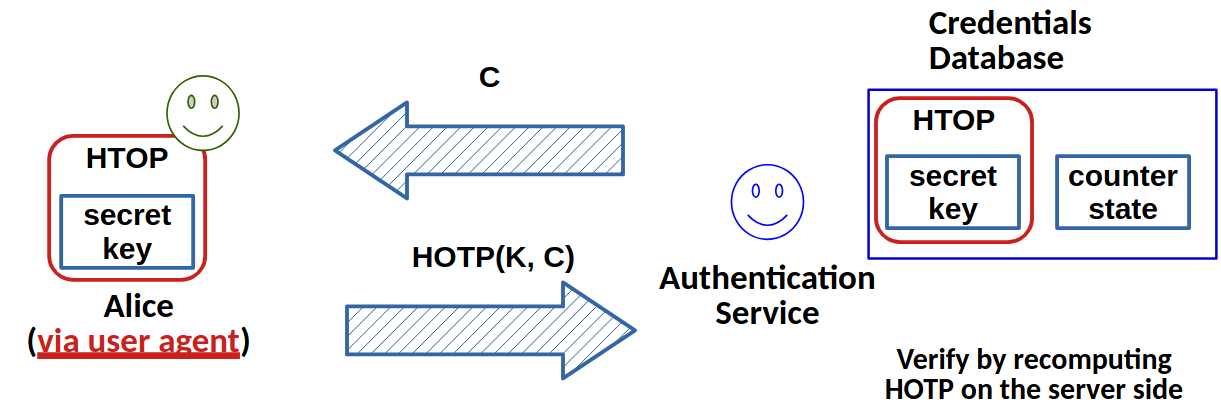
\includegraphics[width=0.65\textwidth]{img/hotp.png}
        \end{figure}

        Questo tipo di protocollo prova che Alice ha \textbf{controllo} sull'informazione secreta, ma potrebbe anche non averla - il segreto potrebbe essere gestito da un ``device'' differente tipo \textbf{\textit{Trust Platform Module - TPM}}. È possibile evitare di inviare esplicitamente la \textit{challenge} se abbiamo una sorgente comune (\textbf{variabile}) di informazioni, ad esempio il \textbf{tempo}.

        \begin{figure}[h]
            \centering
            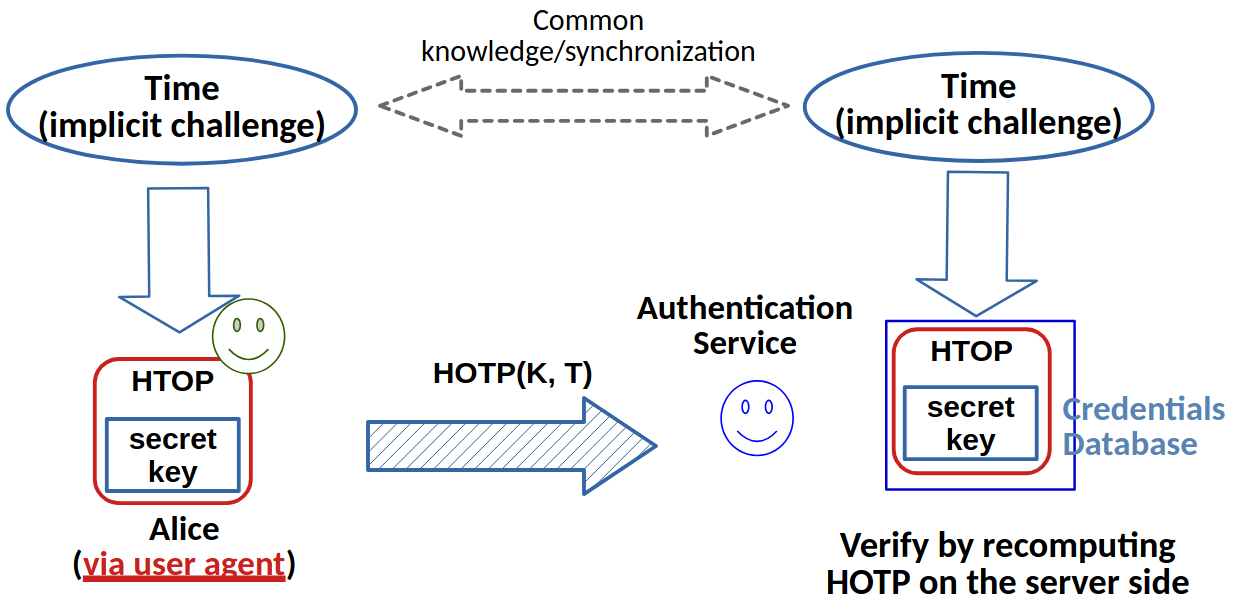
\includegraphics[width=0.65\textwidth]{img/hotp_1.png}
        \end{figure}

    \item \textbf{TOTP, RFC6238 - \textit{Time-Based One-Time Password}}: è un caso speciale dell'\textbf{HOTP}, infatti $\text{HTOP}(k, t) = \text{TOTP}(k, t)$ dove $t$ esprime \textbf{\textit{time step}} calcolati $t = \lfloor \frac{(\text{CurrentUnixTime} - T_0)}{X}$ dove $T_0$ è un tempo base Unix che decreta dove iniziare il conteggio, $X$ è il parametro che indica gli \textit{step} temporali. Assumiamo che client e server hanno accesso ad un'\textbf{informazione condivisa} - normalmente \textbf{\textit{UTC time}}.
    \end{enumerate}
\end{flushleft}

\section{Password e PIN}

\begin{flushleft}
    Il più semplice sistema di autenticazione richiesto ad un client è quello di fornire le sue credenziali, \textit{username:password}. L'utente invia le sue credenziali (attraverso un canale sicuro), il server esegue una \textit{query} al database per ottenere la password salvata per un certo username e poi effettua il confronto tra quella fornita e quella salvata.

    \smallskip

    \textbf{Definizione}: Le \textbf{password} sono dei segreti ricordabili dagli umani e quindi \textbf{deboli} per definizione. Questo non toglie la possibilità che utenti possano scegliere ``password forti'', ma nella maggior parte degli scenari dobbiamo assumere il contrario.

    \smallskip

    Andiamo a definere cosa vuol dire ``\textbf{segreto debole}'': un avversario può ``indovinare'' il segreto con un numero fattibile di tentativi. Il che può essere dovuto a:
    \begin{itemize}[nosep]
        \item \textbf{\textit{enumeration}}: con molti pochi tentativi, abbiamo un segreto ``molto debole'': \textbf{\textit{dictionary attack}}.
        \item \textbf{\textit{brute-forcing}}: il numero di tentativi diventa non trascurabile, numero limitato di password possibili.
    \end{itemize}

    \smallskip

    \textbf{Password}: segreti a bassa entropia, facilmente memorizzabili. Possono essere scelte corte e con un alfabeto ridotto. Anche password che non sono ``deboli'' possono diventare vulnerabili nel lungo periodo, infatti vengono considerate deboli in termini crittografici. \\
    \textbf{PIN}: segreti a bassa entropia (molto bassa), sono intrinsecamente vulnerabili a \textbf{ricerca esaustiva}, devono essere utilizzati solo in contesti vincolati dall'interfaccia per l'immissione.

    \medskip

    Un avversario può provare ad ``\textbf{indovinare}'' la password di un utente che sa che esiste, andando a fare richieste ripetute fino a che non riesce ad ottenere il login. 

    \begin{figure}[h]
        \centering
        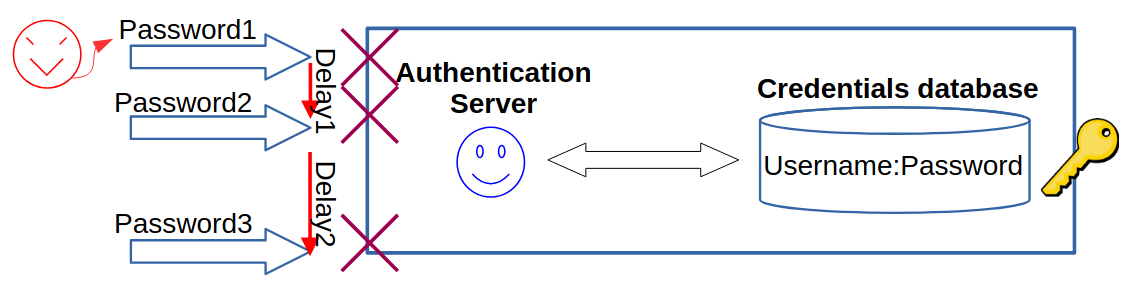
\includegraphics[width=0.55\textwidth]{img/int_attack.png}
        \caption{\textbf{\textit{Interactive Attack}}}
    \end{figure}

    Per conoscere il risultato del tentativo l'attaccante deve interagire con il server, per attenuare l'attacco il server può e deve applicare un \textbf{\textit{delay}} tra i tentativi del login per mitigare l'attacco di \textit{brute-force}. Con i \textbf{PIN} l'idea è la medesima, ma siccome sappiamo che il \textbf{PIN} è molto più debole è quindi necessario inserire un \textbf{numero massimo di tentativi} e in caso di mancata autenticazione si ricade in un altro sistema di \textbf{AuthN} più ``forte'' (\textbf{\textit{fallback}}). \\

    Libreria \textbf{python} per \textbf{HOTP} e \textbf{TOTP}: \textbf{\textit{pyotp}}.

\end{flushleft}

\section{Password Protection against Data Breaches}

\begin{flushleft}
    Focalizziamoci sul problema di \textbf{protezione delle password}, assumendo che il server sia completamente \textbf{compromesso} dall'avversario. I vincoli intrinsici che espone questa assunzione sono:
    \begin{enumerate}[nosep, start=0]
        \item non bisogna salvare le password in chiaro
        \item bisogna essere protettti conto \textit{pre-computational attacks}
        \item aumentare al protezione contro le password deboli.
        \item essere in grado di difenderci contro \textbf{attacchi ``specializzati''}
    \end{enumerate}

    \medskip

    \textcolor{red}{\textbf{[0] Non salvare le password in chiaro}}: salvare le password in chiaro comporta che se il server è completamente compromesso e l'attaccante ha accesso a tutte le coppie \textit{(username, password)}. La sua speranza è il riutilizzo della stessa coppia per altri applicazioni.

    \smallskip

    \textcolor{red}{\textbf{[1] Proteggere le credenziali nel database utilizzando le \textit{hash function}}}: in questo modo sarà possibile fare il confronto con il \textit{digest} salvato e il \textit{digest} ottenuto dall'applicazione della funzione hash alla password immessa dall'utente per autenticarsi. Siccome la funzione hash è \textbf{unidirezionale} se l'attaccante ha compromesso il sistema non sarà capace a partire dal \textit{digest} ottenere la password (\textbf{\textit{one-way}}).
    \begin{itemize}[nosep]
        \item se l'attaccante ottiene $H(p)$ dove $p$ è la password dell'utente, l'unico modo per ottenere $p$ è trovare una funzione inversa $H^{-1}$ (che dalle proprietà delle \textit{hash function} dovrebbe essere impossibile) oppure riuscire a trovare una password $p'$ (tramite \textbf{attacco esaustivo} sullo spazio delle password o con un \textbf{attacco a dizionario}) il cui \textit{digest} è uguale ad $H(p) = H(p')$
        \item quindi l'attaccante fallisce fintanto che $h$ è una funzione crittografica sicura? se le password venissero scelte come \textbf{chiavi crittografiche} allora \textbf{si}, nel caso in cui vengano scelte da un utente non paranoico allora \textbf{no}.
        \item infatti l'attaccate riesce a fare un \textbf{\textit{pre-computation attack}} potrebbe diminuire il tempo per trovare delle collisioni, soprattutto in caso di password corte; tipico esempio di \textbf{compromesso-spazio tempo} (possono essere violate anche password buone).
        \item non è possibile difendersi se l'avversario compromette la logica applicativa, quindi unicamente in caso di \textbf{\textit{data breach}}.
    \end{itemize}
\end{flushleft}
\begin{boxA}
    \textcolor{red}{\textbf{\textit{Pre-computation Attack to Credential Database}}}

    \begin{center}
        
\includegraphics[width=\textwidth]{img/pre_attack_pwd.png}
    \end{center}

    L'obiettivo dell'attaccante è quello di ottenere una pre-immagine della password con l'hash non appena accede al database. Una possibilità sarebbe quella di \textbf{pre-calcolare} tutte le possibili password e il \textit{digest} corrispondente, la problematica di questa tipologia di approccio è che richiederebbe un mole memoria infattibile $\rightarrow$ \textbf{\textit{rainbow tables}} permettono di pre-calcolare attachi agli hash delle password senza dover memorizzare tutte le possibili corrispondenze per un dato \textit{domain}, la loro dimensione dimenta infattibile per lunghi input (16bytes alfanumerici).

    \smallskip

    $\Delta(t_0, t_1) \rightarrow 0$ in modo tale da limitare il tempo in cui un attaccante proverà l'\textit{offline cracking}, tramite il monitoraggio del traffico, del \textit{dark web} per osservare le \textit{disclosure} dei \textit{data breach} e segnalazione da parte di altri utenti.
\end{boxA}

\begin{flushleft}
    \textcolor{red}{\textbf{[2] Protezzione contro \textit{pre-computational attack} attraverso il \textit{Salt}}}: la difesa migliore è rendere \textbf{randomico l'\textit{hash function}}. Per ogni utente la password viene hashata con un differente valore \textbf{unico e randomizzato}, chiamato \textbf{\textit{salt}}, che viene salvato insieme al \textit{digest} nel database. Per ogni utente la sua riga di autenticazione sarà quindi formata da: 
    
    {\centering
        | \textit{username} | \textbf{\textit{salt}} | \textbf{\textit{hash(salt, password)}} |
    \par}

    In questo moto l'attaccante non può costruire la \textbf{\textit{rainbow table}} fino a che non ottiene il valore del \textbf{\textit{salt}}, ma siccome il valore del \textit{salt} viene ottenuto dall'attaccante durante la fase di \textbf{\textit{data breach}}, la generazione della \textit{rainbow table} avviene \textbf{online}, se si utilizzasse lo stesso \textit{salt} per più password una \textit{rainbow table} permetterebbe di aumentare l'efficenza del \textit{cracking} anche se online. In ogni caso l'attaccante è comunque capace di violare agilmente password deboli.

    \smallskip

    \textcolor{red}{\textbf{[2a] \textit{Secret Salt}}}, anche noto come \textbf{\textit{pepper}} è ottenibile dividendo l'\textbf{\textit{authentication server}} da un compomente esterno che genera il \textbf{\textit{secret salt}}, attraverso una \textbf{KDF}:

    {\centering
        \textbf{pepper} = \textbf{KDF}(\textbf{\textit{key}}, dimensione, ``\textbf{\textit{user}} || '\textbf{versione}')
    \par}
    
    Se viene compromesso questo componente esterno il \textit{fallback} è tornare all'utilizzo del \textbf{\textit{public salt}}, è anche importante ricordare che non è una soluzione semplice ed è difficilmente integrabile con framework di sviluppo web.

    \smallskip

    \textcolor{red}{\textbf{[3] Difendersi contro le password ``deboli''}}: introduciamo un nuovo \textbf{schema crittografico}: \textbf{\textit{password-based hash functions}}, chiamate \textcolor{red}{\textbf{\textit{PBKDF - Password-Based Key Derivation Functions}}}. Il loro obiettivo è quello di \textbf{aumentare} il tempo di esecuizione del calcolo dell'hash (\textit{slow down}) in modo tale che comunque rimanga \textbf{moderato}, ma che il suo inverso sia comunque \textbf{infattibile}. L'idea non è quella di bloccare completamente gli attacchi \textit{offline} delle password, se la password è debole è imposibile senza modificare anche l'architettura, ma cercare di \textbf{rallentarli} attacchi esaustivi \textbf{senza compromettere l'esecuzione del servizio legittimo}.
    \begin{itemize}[nosep]
        \item i ritardi devono essere valutati e aggiornati nel tempo in base all'hardware disponibile e al suo costo.
        \item se l'attaccante vuole andare più veloce, deve spendere di più.
    \end{itemize}

    Alcuni esempi di \textbf{PBKDF}:
    \begin{enumerate}[nosep]
        \item \textbf{PBKDF1}: procedura iterativa: $\underset{\text{n volte}, \; n \simeq 10^6}{\underbrace{H(H(...(H(}}\text{salt}, \text{password}))))$
        \item \textbf{PBKDF2}: in alcuni scenari potrebbe essere necessario utilizzare questa funzione perché approvata da molti standard.
        \item \textbf{Bcrypt}: supportata, comunemente, in scenari \textit{open-source}, anche questa ha un approccio iterativo.
    \end{enumerate}

    \smallskip

    \textcolor{red}{\textbf{[4] Difendersi contro attacchi ``specializzati''}}: gli attacchi specializzati utilizzano \textbf{hardware dedicato} per riuscire ad annullare (rendere trascurabile) il \textbf{gap} introdotto da funzioni ``lente''. Cercando, ad esempio, rendere le \textbf{PBKDF egalitarie} ovvero standardizzare nel tempo l'esecuzione indipendentemente dall'hardware sottostante.
    \begin{itemize}[nosep]
        \item negli anni '90 gli attaccanti avevano lo stesso hardware.
        \item negli anni '00 gli attaccanti utilizzavano le GPU.
        \item negli anni '10 gli attaccanti iniziano ad utilizzare hardware dedicati.
    \end{itemize}
    Il ritardo introdotto con le \textbf{PBKDF} è reso inutile visto il crescente gap di risorse (sia computazionali che economiche) tra gli attori legittmi e avversari.

    \smallskip

    Abbiamo detto che per mitigare queste tipologie di attacchi bisogna rendere le \textbf{PBKDF \textcolor{red}{egalitarie}}, idealmente, l'attaccante non deve essere capace di sfruttare il vantaggio che potrebbe dare architettura specializzate per ogni calcolo rispetto ad un attore legittimo.

    \smallskip

    \textcolor{red}{\textbf{memory-hard hash functions}}: siccome l'hardware dedicato normalmente vuol dire estremamente parallelizzato, ma normalmente queste disposibitivi (ad esempio GPU) hanno molta meno memoria rispetto ad una classica CPU. Pertanto se progettiamo un algoritmo che impieghi quanto più tempo se gli viene messa a disposizione quanta meno memoria evitiamo che gli aggressori possano forzarli in modo più efficiente rispetto agli attori legittmi. In sostanza \textbf{sono molto più lenti da calcolare se viene utilizzata poca memoria}.

    \begin{figure}[h]
        \centering
        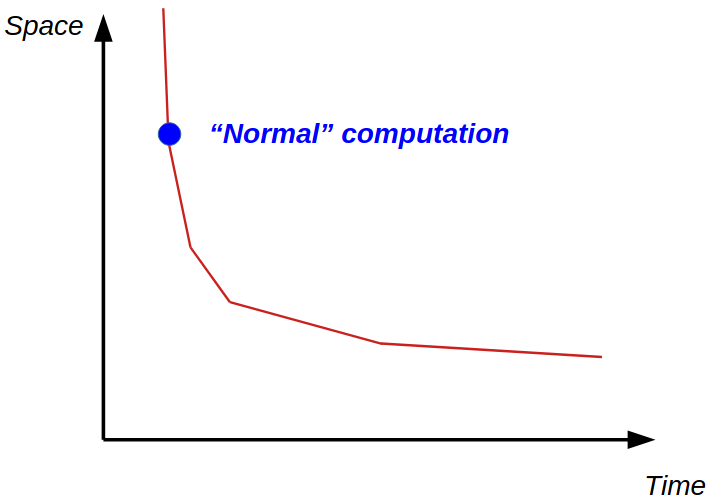
\includegraphics[width=0.35\textwidth]{img/mhf.png}
    \end{figure}

    Il primo algoritmo di questo tipo era \textbf{Scrypt} considerato sicuro, ma soffriva di due svantaggi: era vulnerabile ad una certa categoria di \textit{timing attacks} e il \textit{gap} tra attaccante e attore legittimo non era molto alto. \\
    Venne fatta una competizione per cercare un nuovo algoritmo (\textbf{\textit{password hasing competition}}) e nel 2015 il vincitore \textbf{Argon2} divenne lo standard per questo tipo di circostanze.
    \begin{itemize}[nosep]
        \item \textbf{Argon2i}: l'esecuzione è indipendente dal tempo rispetto agli input consigliata per l'utilizzo nei protocolli a chiave basati su password.
        \item \textbf{Argon2d}: è molto più forte, ma è dipendente dal tempo per quanto riguarda gli input, suggerito per l'uso di schema \textbf{PoW} o quando gli attacchi temporizzati non sono un problema.
        \item \textbf{Argon2id}: unisce le prime due \textit{mode of operation} (ibrido, spesso usato come default).
    \end{itemize}
    Parametri per \textbf{Argon2} :
    \begin{itemize}[nosep]
        \item \textbf{input}: la password inserita.
        \item \textbf{salt}: normalmente o 8 o 16 bytes.
        \item \textbf{\textit{time-cost}}: controlla il tempo di esecuzione (è simile al numero di replicazioni negli approcci iterativi); nel caso di esecuzioni per l'autenticazione \textit{online} siamo nel range 0.5-1.0 secondi, mentre per operazioni \textit{offline} anche più alto.
        item \textbf{\textit{memory}}: quantità di memoria richiesta per il calcolo ``normale'' (ad oggi il minimo per fine autenticativo 64MB, ma si può utilizzare anche 1GB per applicazioni critiche di sicurezza).
        \item \textbf{\textit{parallelism}}: numero di unità di calcolo parallele (anche se dipendenti).
        \item \textbf{\textit{output size}}: lunghezza del \textit{digest} (di default è 16 bytes).
    \end{itemize}
\end{flushleft}
\chapter{Asymmetric Cryptography}

\begin{flushleft}

    \begin{figure}[h]
        \centering
        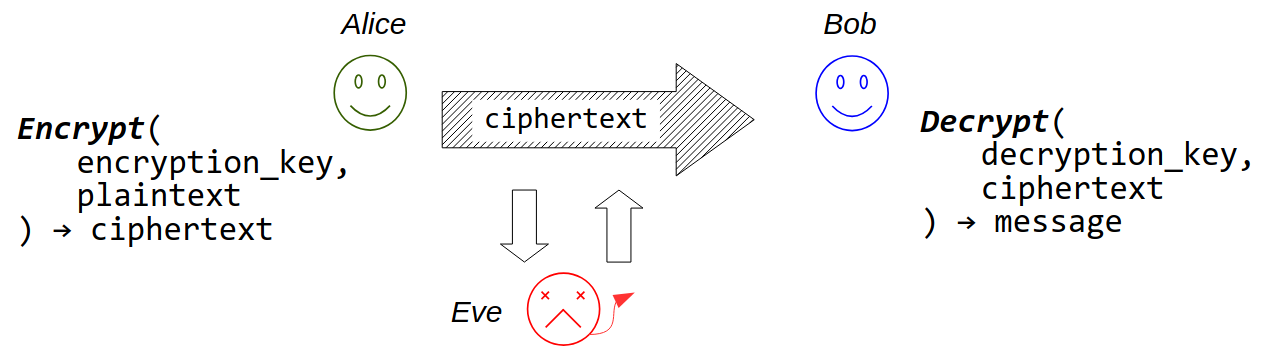
\includegraphics[width=\textwidth]{img/asym_crypto.png}
    \end{figure}

    Nella \textcolor{red}{\textbf{crittografia asimmetrica}} Alice e Bob utilizzano due chiavi differenti, infatti la \textit{encryption key} $\neq$ \textit{decryption key}, normalmente la chiave di cifrature è la pubblica e quella di decifrazione la privata. Il nome \textbf{asimmetrico} deriva dal fatto che dai requisiti per la distribuzione delle chiavi alle entità che partecipano nella comunicazione.

    \smallskip

    \textcolor{red}{\textbf{Coppia di Chiavi}}: nella crittografia asimmetrica è presente una \textbf{\textit{key pairs}} ovvero una coppia di due chiavi diverse, chiamata una \textbf{chiave secreta} (\textbf{\textit{secret key}}) e l'altra \textbf{chiave pubblica} (\textbf{\textit{public key}}). Queste due chiavi sono diverse, ma \textbf{matematicamente legate in maniera univoca}

    {\centering
        \textbf{\textit{secret key (sk)}} $\leftrightarrow$ \textbf{\textit{public key (pk)}}
    \par}

    Normalmente la \textit{secret key} è conosciuta unicamente da un'entità, mentre la \textit{public key} viene distribuita a tutti gli altri. È possibile calcolare la \textbf{pk} partendo dalla \textbf{sk}, ma non il viceversa.

    \smallskip

    Gli schemi crittografici collegati (derivati) con la crittografia simmetrica sono:
    \begin{itemize}[nosep]
        \item \textbf{\textit{digital signature}}
        \item \textbf{\textit{asymmetric encryption}} $\rightarrow$ \textbf{\textit{key encapsulation}} per \textbf{\textit{hybrid encryption}}
        \item (\textit{two party}) \textbf{\textit{key exchange (KEX)}} $\rightarrow$ \textbf{\textit{Authenticated Key Exchange}}
    \end{itemize}

    \smallskip

    \textbf{Crittografia asimmetrica} permettere di rispettare il vincolo di \textbf{confidenzialità}, permette infatti di cifrare il messaggio senza sapere la chiave segreta, ma il destinatario non ha modo di conoscere chi ha cifrato il messaggio.

    \medskip

    \textcolor{red}{\textbf{Crittografia ibrida}} \\
    L'idea è quella di incapsulare una chiave di crittografia simmetrica dentro ad un algoritmo asimmetrico:
    \begin{enumerate}[nosep]
        \item viene generata una chiave simmetrica \textbf{\textit{dek (data encryption key)}}
        \item il tutto viene incapsulato utilizzando uno schema asimmetrico attraverso l'applicazione di un \textbf{\textit{key incapsulation method (kem)}}
        \item dopo aver cifrato il messaggio con la \textbf{dek} attraverso uno schema crittografico simmetrico (ad esempio \textbf{AEAD}) viene inviato.

        \begin{figure}[h]
            \centering
            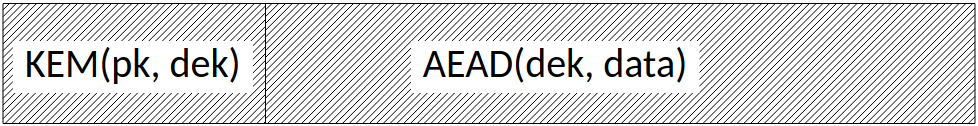
\includegraphics[width=0.75\textwidth]{img/hybrid_enc.png}
        \end{figure}
    \end{enumerate}
    La decifrazione viene applicata in maniera inversa, si decifra la \textbf{dek} con la funzione di decifrazione asimmetrica per poi decifrare il messagio con la \textbf{dek}. Può essere integrata con \textbf{firma digitale} per garantire \textbf{autenticità}.

    \medskip

    \textcolor{red}{\textbf{Firma Digitale}} \\
    In questo caso la \textbf{firma} del dato è fatta da Alice calcolando $\text{signature} = \text{sign}(\text{alice}_{sk}, \text{data})$ e viene verificata da Bob tramite $\{0, 1\} \leftarrow \text{verify}(\text{alice}_{pk}, \text{data}, \text{signature})$ in questo modo è possibile avere garanzie di \textbf{autenticità} nei settaggi asimmetrici, ma conseguentemente permette anche la garanzia su:
    \begin{itemize}[nosep]
        \item chiunque può verificare la \textit{signature} $\rightarrow$ \textbf{\textit{public verifiability}} (assumendo la correttezza della chiave pubblica).
        \item soltanto un'entità conosce il segreto: \textbf{non ripudio} (\textbf{\textit{non repudiability}}).
    \end{itemize}

    \medskip

    \textcolor{red}{\textbf{(secure) \textit{Key Exchange Protocol}}} \\
    Cercano di risolvere il \textbf{problema della distribuzioni delle chiavi} nelle configurazioni a \textbf{crittografia simmetrica}. Alice e Bob vogliono comunicare su un \textbf{canale insicuro} una chiave simmetrica condivisa senza nessuna conoscenza pregressa, per ora assumiamo che l'avversario sia \textbf{passivo}.
    
    \newpage

    \textcolor{red}{\textbf{\textit{Authenticated Key Exchange Protocol}}} \\
    Possiamo identificarla come l'unione di un \textbf{protocollo di scambio di chiavi} con la \textbf{firma digitale}, in questo caso possiamo differenziare:
    \begin{itemize}[nosep]
        \item \textbf{\textit{Server-side authenticated}}: solo il client deve verificare autenticità del server (esempio sito web).
        \item \textbf{\textit{Mutually-Authenticated}}: entrame le entità devono verificare l'autenticità dell'altra.
    \end{itemize}
    Nel caso di \textbf{\textit{Key distribution}} per \textbf{KEX} in base al \textbf{tipo} e al \textbf{contesto} di utilizzo è possibile distribuire una o entrambe le chiavi pubbliche che possono essere \textbf{permanenti} o \textbf{temporanee}.

    \begin{figure}[h]
        \centering
        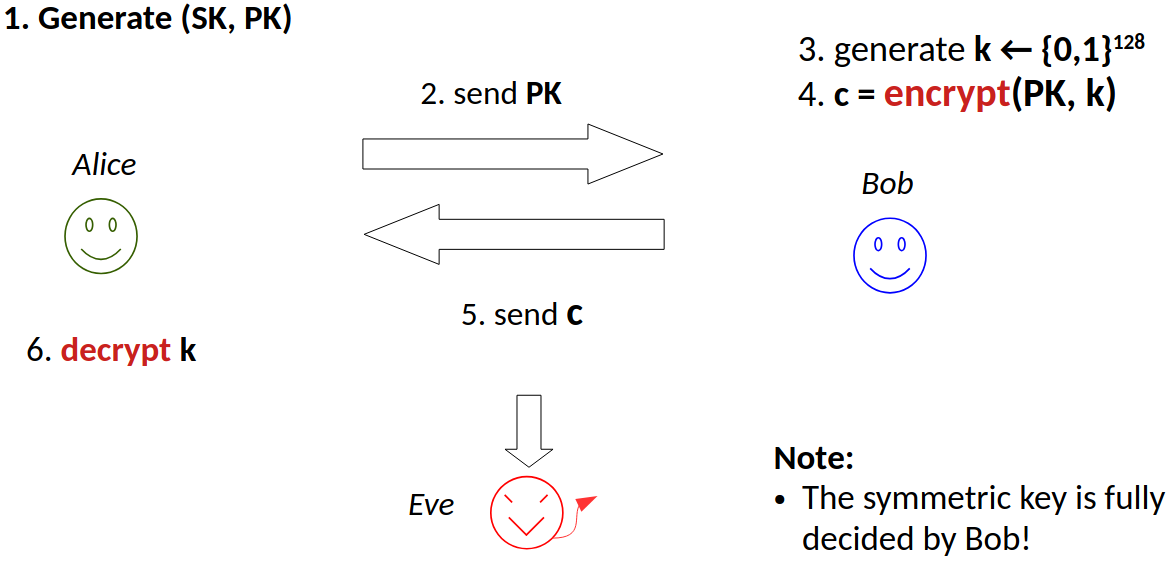
\includegraphics[width=0.75\textwidth]{img/kex.png}
        \caption{Possibile scambio di chiavi via crittografia asimmetrica}
        \label{fig:kex}
    \end{figure}

    In Fig. \ref{fig:kex} la \textit{encrypt} e la \textit{decrypt} sono riferiti allo schema asimmetrico di crittografia. In questi contesti possono comunque esserci dei problemi legati all'\textbf{autenticità della distribuzione} (sotto un attacco attivo, un avversario potrebbe distribuire chiavi false). E anche problemi legati alla \textbf{\textit{privacy}} infatti chiunque può utilizzare le nostre chiavi pubbliche (in alcuni contesti come quello della firma digitale, può essere un problema). Esistono schemi alternativi che permettono di imporre l'\textbf{anonimato}.
    
\end{flushleft}

\newpage

\section{Trapdoor One-Way Function}

\begin{flushleft}
    \textcolor{red}{\textbf{Primitive in Crittografia Simmetrica e Asimmetrica}}
    \begin{center}
        \begin{minipage}[t]{0.45\textwidth}
            \textbf{Crittografia Simmetrica}: sono basate principalmente sull'\textbf{analisi euristica}. Le funzioni sono indistinguibili da oggetti ideali come le \textbf{PRF} o \textbf{PRP}, se guardiamo il \textit{design} interno possiamo osserva la costruzione di questi blocchi su \textbf{\textit{bit-wise operation}}.
        \end{minipage}
        \hfill
        \begin{minipage}[t]{0.45\textwidth}
            \textbf{Crittografia Asimmetrica}: sono basate su - maggiormente strutturati - \textbf{problemi e algortmi matematici}. \\
            $\rightarrow$ \textbf{\textit{trapdoor one-way function}}
        \end{minipage}
    \end{center}

    Le \textbf{\textit{one-way function}} sono funzioni $f$ che sono \textbf{efficenti} da calcolare (costo polinomiale), ma che la loro funzione inversa $f^{-1}$ è \textbf{inefficente} (costo esponenziale). In crittografia simmetrica ne abbiamo già viste alcune, tra cui: le \textit{hash function} e i \textit{stream cipher} che sono \textbf{veloci}, ma completamente non strutturate e con un \textbf{comportamente impredicibile}, cosa che invece è richiesta in questo contesto. Dobbiamo ricercare tipologie di problemi matematici noti che rispecchiano queste esigenze, in modo da conoscerne il comportamento e poterlo sfruttare, ricercando quei problemi che hanno un \textbf{costo algoritmico} non trascurabile.
    \begin{itemize}[nosep]
        \item \textbf{Logaritmo discreto} (Logaritmo nei gruppi ciclici di ordine un primo): che possono basarsi su un \textbf{\textit{finite field (ff)}} costruito su un \textbf{primo intero} oppure su gruppi costruiti su \textbf{curve ellittiche}
        % campo non mi sembra corretto -> anello
        \item \textbf{rsa}: \textit{Rivest-Shamir-Adleman} che basano il problema su un \textbf{campi} di ordine \textbf{composti}, dove i fattori sono due primi di grandi dimensioni.
    \end{itemize}

    \begin{figure}[h]
        \centering
        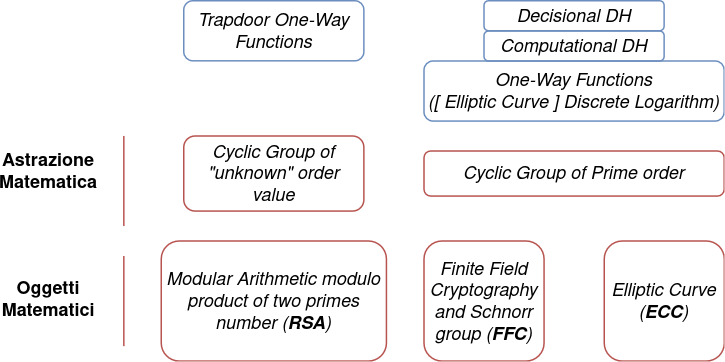
\includegraphics[width=0.75\textwidth]{img/md_crypto.png}
    \end{figure}

    Sia \textbf{RSA} che il \textbf{problema del logaritmo discreto} sono efficentemente invertibili con i \textbf{computer quantistici} (attraverso l'applicazione dell'algoritmo di \textbf{Shor}). Schemi di crittografia \textbf{\textit{post-quantum}} (promessi) si basano su problemi matematici legati a \textbf{\textit{Codes}} e \textbf{Reticoli} (\textbf{\textit{Lattices}}).
\end{flushleft}

\section{Diffie Hellman Conjectures}

\begin{flushleft}
    Consideriamo il \textbf{gruppo ciclico moltiplicativo} $\mathbb{Z}_{11}^{\times} = \{0, 1, 2, 3, 4, 5, 6, 7, 8, 9, 10\}$ e consideriamo gli elementi $2$, $3$ e $10$ andando a calcolarci il \textbf{sottogruppo ciclico} generato da questi elementi:
    \begin{itemize}[nosep]
        \item il generatore $2$ permette di ottenere il sottogruppo $\{1, 2, 3, 4, 5, 6, 7, 8, 9, 10\} \subseteq \mathbb{Z}_{11}^{\times}$
        \item il generatore $3$ permette di ottenere il sottogruppo $\{1, 3, 4, 5, 9\} \subset \mathbb{Z}_{11}^{\times}$
        \item il generatore $10$ permette di ottenere il sottogruppo $\{1, 10\} \subset \mathbb{Z}_{11}^{\times}$
    \end{itemize}
    Diremo che l'\textbf{l'ordine} del sottogruppo ottenuto dal generatore $3$ è \textbf{5} e viene definito come \textbf{\textit{Schnorr group}}. Dato un $p$ primo scrivibile come $p = 2 \cdot q + 1$ con $q$ primo, $p$ viene definito \textbf{\textit{safe prime}} (o \textbf{\textit{strong prime}}), con $p$ che sono definiti in questo modo possiamo generare 3 sottogruppi di ordine differente, rispettivamente di ordine $2$, $q$ e $2q$ (ovvero $p-1$). \\
    In algoritmi crittografici le cui primitive si basano su gruppi di ordine $p$ una scelta sbagliata del \textbf{generatore} può causare \textbf{problemi di sicurezza}.

    \smallskip

    La funzione \textbf{\textit{one-way}} che possiamo descrivere è quella del \textbf{logaritmo discreto} su un \textbf{gruppo ciclico di ordine primo}, consideriamo un generatore $g$ di un gruppo ciclico di ordine $p$ e consideriamo un $g^a \; \text{con} \; a \in \mathbb{Z}_p^{\times}$ sarà computazionalmente oneroso calcolarsi il valore $a$.

    \begin{itemize}[nosep]
        \item problema del \textbf{logaritmo discreto}: noto $g^a$ sarà difficilemnte calcolabile $a$.
        \item \textbf{\textit{computational Diffie-Hellman}} dati $g^a$ e $g^b$ sarà oneroso calcolarsi $g^{ab}$.
        \item \textbf{\textit{decisional Diffie-Hellman}} dati $g^a$ e $g^b$ sarà computazionalmente difficile distinguere $g^{ab}$ da $g^r$ dove il valore $r$ è random.
    \end{itemize}

    \newpage

    \textcolor{red}{\textbf{Curve Ellittiche}}
    \begin{itemize}[nosep]
        \item \textbf{forma di Weistrass}: $y^2 = x^3 + ax + b$
        \item \textbf{Curve Ellittiche di Edwards}:
        \begin{math}
            \begin{cases}
                x^2 + y^2 = a^2 + a^2x^2y^2 \\
                x^2 + y^2 = 1 + dx^2y^2
            \end{cases}
        \end{math}
    \end{itemize}

    \medskip

    Anche nel caso dell'applicazione di forme geometriche come le curve ellittiche, bisogna sempre ricordarsi che noi lavoreremo con numeri interi modulari.

    \medskip

    \begin{figure}[h]
        \centering
        \begin{minipage}[t]{0.45\textwidth}
            \centering
            Forma di Weistrass nell'insieme $\mathbb{R}$ \\
            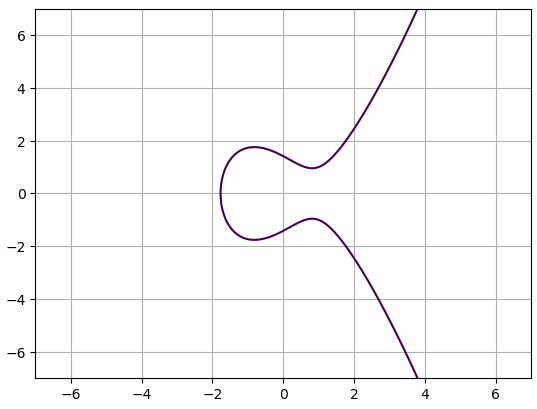
\includegraphics[width=\textwidth]{img/ec_wform.png}
            \caption{$y^2 = x^3 - 2x + 2$}
        \end{minipage}
        \hfill
        \begin{minipage}[t]{0.45\textwidth}
            \centering
            Forma di Weistrass nell'insieme $\mathbb{Z}_{149}$ \\
            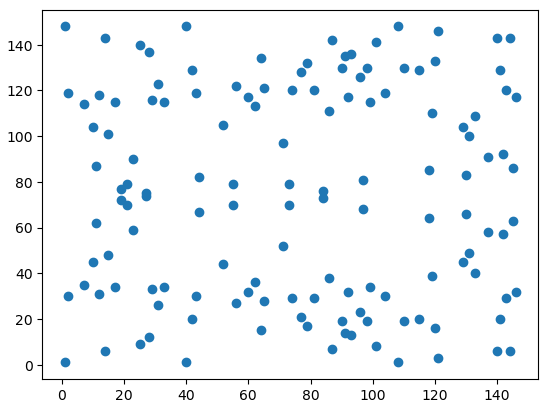
\includegraphics[width=\textwidth]{img/ec_modform.png}
            \caption{$y^2 = x^3 - 2x +2$}
        \end{minipage}
    \end{figure}

    I gruppi ciclici possono essere astratti in notazione \textbf{moltiplicativi} e \textbf{additivi}
    \begin{itemize}[nosep]
        \item \textbf{gruppi ciclici su \textit{FFC} che adottano una notazione moltiplicativa} $G_1 \cdot G_2$ è il prodotto di due interi $G_1$ e $G_2$ modulo $q$. $g^a$ con $g < q$ (intero), mentre $a < p$ (interi), le operazioni sono delle esponenziazioni modulo $q$.
        \item \textbf{gruppi ciclici su \textit{ECC} tipicamente adottano una notazione additivia} $G_1 + G_2$ è la somma di due \textbf{punti}, mentre $a \cdot G$ dove $G$ è un punto sulla curva ellittica (chiamato \textbf{\textit{base point}}), $a$ invece è uno scalare, l'operazione è quella della moltiplicazione scalare di un punto sulla curva.
        \begin{itemize}[nosep]
            \item il problema del logaritmo discreto su curve ellittiche è calcolare $a$ dato $a \cdot G$
            \item \textit{computational Diffie-Hellman} su ECC è calcolare $(a + b) \cdot G$ da $a \cdot G$ e $b \cdot G$
        \end{itemize}
    \end{itemize}
    
    \smallskip

    \textcolor{red}{\textbf{\textit{(Extra) but suggested}}} \\
    Un \textbf{punto} $P$ è formato da due coordinate $(P_x, P_y)$ ognuna delle coordinate appartiene al \textbf{campo} $\mathbb{Z}_p$ come la anche la curva. Le curve ellittiche in crittografia sono \textbf{simmetriche rispetto ad almeno un asse} (nel caso delle \textbf{curve di Edwards} ad entrambi). $-P = (P_x, -P_y)$. \\
    La rappresentazione di un punto può essere quindi \textbf{compressa} esprimendo una delle due coordinate come un bit singolo: $P = (P_x, \{0, 1\})$, infatti $P_y$ può essere ricalcolato utilizzando l'equazione della curva e il \textbf{bit} permetterà di definire il \textbf{segno}: $+ \rightarrow [0, \frac{p - 1}{2}]$ e $- \rightarrow [\frac{p - 1}{2} + 1, p - 1]$.

    \smallskip

    In certi protocolli un attaccante potrebbe fornire un \textbf{punto} $p \notin E_p(a, b)$ ovvero che le coordinate $(P_x, P_y)$ non soddisfano l'equazione della curva, oppure fornire un \textbf{punto valido} $p \in E_p(a, b)$ ma non \textbf{appartiene al gruppo crittografico} (appartiene ad un sottogruppo di ordine ``piccolo''). \\
    In entrambi gli attacchi è possibile utilizzare \textbf{proprietà matematiche} per rompere queste implementazioni incorrette, è possibile prevenirle sia a livello implementativo (aggiungendo controlli sulla validità del punto) o a livello di progettazione.

    \smallskip

    \textcolor{red}{\textbf{\textit{(extra)} Diversi Sistemi di Coordinate}} \\
    Lavorare con le \textbf{curve ellittiche} richiede molte operazioni aritmetiche sui punti. Alcuni sistemi di coordinate permettono di velocizzare i calcoli (ad esempio evitare divisioni modulari, che sono lente) a scapito di occupare più spazio in memoria (\textbf{\textit{trade-off} spazio/tempo})
    \begin{itemize}[nosep]
        \item \textbf{coordinate \textit{affine}} (``\textit{native}''): questo è il modo banale di rappresentazione $P(P_x, P_y)$, dove $P_x, P_y \in \mathbb{Z}_p$ e che soddisfano l'equazione della curva. È possibile \textbf{comprimerle} andando ad inviare una coordinata e un bit che rappresenta il segno dell'altra.
        \item \textbf{\textit{projective}} (proiettive): qui viene rappresentato ogni punto come $(X, Y, Z)$ dove $x = \frac{X}{Z}$ e $y = \frac{Y}{Z}$ in questo modo si possono eseguire operazioni tra punti senza dover fare divisioni modulo $p$, d'altro canto occupano più memoria e le formule sono più complicate.
        \item \textbf{\textit{Jacobian}} $(X, Y, Z)$ in questo caso avremo che $x = \frac{X}{Z^2}$ e $y = \frac{Y}{Z^2}$ sono ottimizzate per curve nella forma di Weistrass.
        \item \textbf{\textit{Modified Jacobian}} $(X, Y, Z, \alpha)$ come le precedenti, ma viene tenuto in memoria un valore precomputato per evitare calcoli ripetuti durante il \textbf{doubling}, vengono usate per migliorare le performance, specialmente in ambienti con risorse limitate o ottimizzazioni hardware.
    \end{itemize}

    La differenza nella rappresentazione non cambiano il punto matematico della curva. Per confrontare se due punti sono uguali, normalmente bisognerebbe tornare in coordinate affini (bisognerebbe fare la divisione, che però è molto costosa) è quindi possibile utilizzare dei ``trucchi'' algebrici per confrontare direttamente. Ad esempio in proiettivo:

    {\centering
        $X_1 \cdot Z_2 \equiv_p X_2 \cdot Z_1 \; \rightarrow \; x_1 = x_2$
    \par}

    La differente rappresentazione dei punti permette di ottimizzare le tre operazioni che normalmente vengono eseguite sulle curve ellittiche: \textbf{\textit{point addition}}, \textbf{\textit{point doubling}} e \textbf{\textit{scalar multiplication}}. In coordinate affini ogni somma di punti richiede un'inversione $\mod p$ che è ``molto lenta'' in coordinate jacobiane o proiettive ognuna di queste operazioni è effettuabile solo con somme e moltiplicazioni e quindi ``molto più veloce''.
\end{flushleft}

\section{RSA Design}

\begin{flushleft}
    Spiegazione di \textbf{\textit{Textbook RSA cryptosystem}}.

    \smallskip
    
    Nella crittografia asimmetrica abbiamo a che fare con oggetti matematici peculiari:
    \begin{itemize}[nosep]
        \item interi minori di numeri primi ($p$ in DH) o non-primi ($n$ in RSA)
        \item diverse dimensioni degli interi (ordine vs. numero di elementi di un gruppo)
        \item coordinate dei punti su una curva
        \item elementi di un gruppo che devono rientrare in sottogruppi specifici
    \end{itemize}
    
    Queste caratteristiche possono causare dei \textbf{limiti}. Pensando alla crittografia simmetrica, sappiamo che una chiave segreta deve appartenere ad un dominio binario dell'informazione con entropia uniformemente distribuita, ma nel nostro caso noi stiamo lavorando in un dominio diverso: quello dei numeri interi. Ma anche dei \textbf{richi di sicurezza}.

    \smallskip

    \textcolor{red}{\textbf{L'Insicurezza di \textit{Textbook RSA}}} \\
    Le proprietà matematiche esplicitate implicano \textbf{\textit{malleability}} (malleabilità) e \textbf{determinismo} - è possibile enumerare l'intero spazio dei messaggi, infatti la chiave di cifratura è pubblica, chiunque ci può accedere.
\end{flushleft}

\section{Diffie-Hellman Key Exchange}

\begin{flushleft}
    \begin{figure}[h]
        \centering
        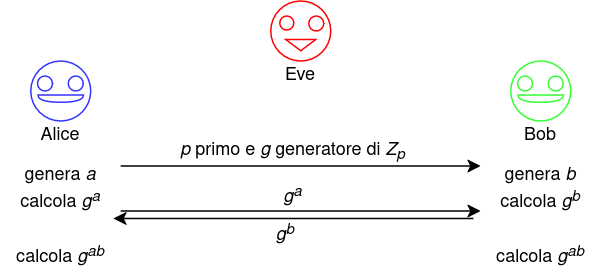
\includegraphics[width=0.55\textwidth]{img/dh.png}
    \end{figure}
    Dove $a$ e $b$ sono i \textbf{segreti temporanei} di Alice e Bob (\textbf{\textit{ephemeral keys}}), mentre $g^a$ e $g^b$ sono i \textbf{contributi pubblici} di Alice e Bob (\textbf{\textit{public contributions}}). Solo Alice e Bob possono calcolare $g^{ab}$, Eve non riesce per via del \textbf{\textit{Computational Diffie-Hellman (CDH)}} e se è valida anche la \textbf{\textit{Decisional Diffie-Hellman}} allora $g^{ab}$ è un segreto ad alta entropia che può essere utilizzato come input di una \textbf{KDF} per generare uno o più \textbf{chiavi simmetriche}. La debolezza di DH è che le parti non sono \textbf{autenticate} $\rightarrow$ \textbf{\textit{Man in the Middle Attack}}. \\
    Eve può svolgere un doppio \textbf{DH \textit{key exchange}} simultaneo con Alice e Bob interporsi nella comunicazione. \textbf{Soluzione}: \textbf{\textit{Authenticated Key Exchange}} le uniche assunzioni sono che Alice [ e Bob ] abbia una coppia di chiavi ($s_k, p_k)$ e che Bob [ Alice ] conosca la chiave pubblica.

    \smallskip

    Lo scambio di chiavi (\textbf{KEX}) può essere ricondotto a un \textbf{KEM (\textit{Key Encapsulation Mechanism})}, e applicando firme digitali a uno scambio di chiavi basato su \textbf{KEM} si ottiene un \textbf{KEX autenticato}. Con Diffie-Hellman (DH), la chiave simmetrica è contribuita da \textbf{entrambe le parti}, mentre con un KEM è decisa da una \textbf{sola parte}. A seconda del contesto, uno può essere preferito all'altro: per scopi generali, DH è la scelta tipica poiché facilita la forward secrecy grazie all'uso di chiavi ephemeral. Tuttavia, il fatto che la chiave venga decisa da un solo lato semplifica l'implementazione di alcune soluzioni di sicurezza, come la \textit{Deep Packet Inspection} su traffico cifrato (una forma di MITM legittimo). Infine, va notato che le primitive post-quantum più promettenti attualmente supportano solo scambi di chiavi basati su KEM.

\end{flushleft}

\section{Digital Signature based on DH Conjectures}

\begin{flushleft}
    \textcolor{red}{\textbf{\textit{Digital Signature Algorithm (DSA)}}}: standard alternativo alla firma di RSA. È basata sul \textbf{logaritmo discreto}, può essere implementata attraverso le curve ellittiche: \textbf{\textit{ECDSA}} (è la ragione per cui viene preferita ad RSA, scala meglio rispetto al livello di sicurezza richiesto). La via più semplice per implementare crittografia con DH è adottare un \textbf{\textit{hybrid design}}, lo standard è \textbf{\textit{Elliptic Curve Integrated Encryption Scheme (ECIES)}}.

    \begin{figure}[h]
        \centering
        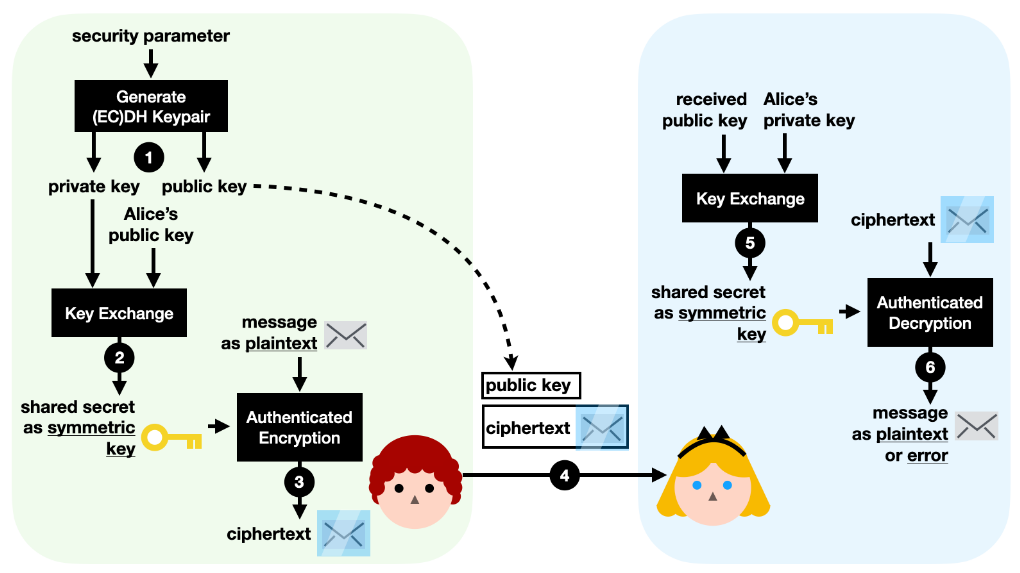
\includegraphics[width=0.85\textwidth]{img/ecies.png}
        \caption{ECIES schema}
    \end{figure}

    \medskip

    \textcolor{red}{\textbf{\textit{Digital Signature based on DH}}}: solo chi conosce il segreto può creare una firma (\textbf{\textit{signature}}) valida, ma dobbiamo distribuire una chiave pubblica che non rileva il segreto e permette di verificare la firma (\textbf{\textit{verify}}). Questa tipologia di firma digitale è del tipo \textbf{\textit{Non-Interactive Zero-Knowledge Proof}} sulla conoscenza dell'esponente segreto. Per verificare la firma il \textbf{\textit{signer}} prova la conoscenza del segreto senza rivelarla ($\neq$ \textbf{commitments} - che viene utilizzato come \textit{subroutine}).

    \begin{figure}[h]
        \centering
        \begin{minipage}[t]{0.45\textwidth}
            \textbf{\textit{Non Interactive Zero Knowledge Proof - NIZKP}} \\
            \textbf{Obiettivo}: permettere ad un \textit{prover} di dimostrare ad un \textit{verifier} di conoscere un certo segreto senza rivelarlo, e senza interazione. \\
            \textbf{Casi d'uso}: firme digitali, prova di range, \textit{blockchain} (zk-SNARKS).
        \end{minipage}
        \hfill
        \begin{minipage}[t]{0.45\textwidth}
            \textbf{\textit{Key Commitment}} \\
            \textbf{Obiettivo}: permettere ad una parte di ``\textbf{impegnarsi}'' su un \textbf{valore segreto} (ad esempio una chiave) in modo che:
            \begin{itemize}[nosep]
                \item non possa essere cambiato (\textit{binding})
                \item l'altro non la può conoscere finché non gli verrà rivelata (\textit{hiding})
            \end{itemize}
            Può essere visto come una busta sigillata crittografica. \\
            \textbf{Casi d'uso}: protocolli \textbf{KEX} per evitare attacchi \textit{MitM}, protocolli di \textit{fair exchange}.
        \end{minipage}
    \end{figure}

    \smallskip

    \textcolor{red}{\textbf{[1] \textit{Zero-Knowledge proof of Secret Exponent}}} dove il \textit{prover} è \textbf{onesto} \\
    
    \begin{figure}[h]
        \centering
        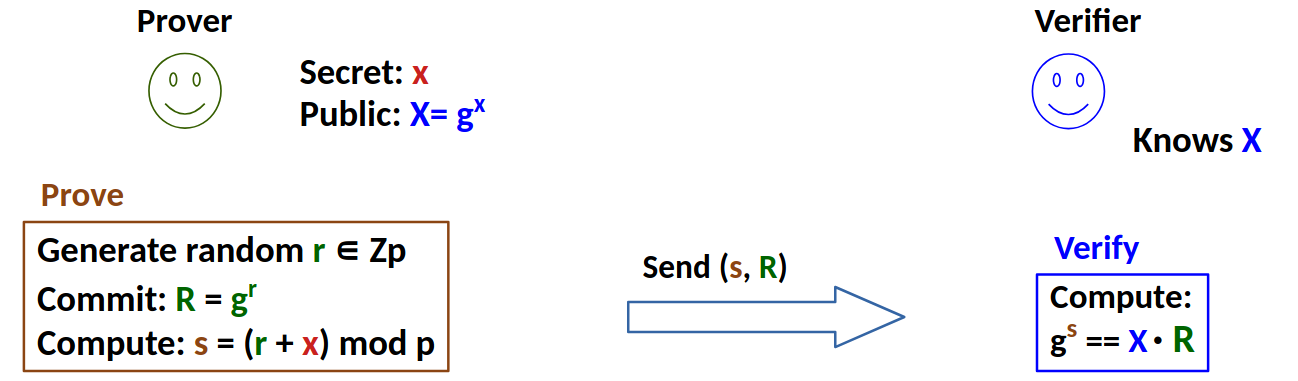
\includegraphics[width=0.95\textwidth]{img/zk_honest_prover.png}
    \end{figure}

    \begin{figure}[h]
        \centering
        \begin{minipage}[c]{0.45\textwidth}
            \textbf{Note}: osserviamo che $p$ definisce l'ordine del gruppo crittografico generato da $g$, $(r + x) \mod p$ garantisce \textbf{confidenzialità} (come un OTP), $r$ è spesso chiamato \textit{nonce} (\textbf{univocità} per la firma), ma deve essere \textbf{segreto} ed \textbf{impredicibile} $\rightarrow$ \textbf{random}, è quindi anche chiamato \textbf{\textit{one-time secret value}} della firma o \textbf{\textit{secret nonce}}.
        \end{minipage}
        \hfill
        \begin{minipage}[c]{0.45\textwidth}
            \begin{align*}
                & \textcolor{olive}{\textbf{Dimostrazione}} \quad & \\
                g^s &\equiv_p X \cdot R \\
                g^{(r + x)} &\equiv_p X \cdot R \\
                g^r \cdot g^x &\equiv_p X \cdot R \\
                R \cdot X &\equiv_p X \cdot R
            \end{align*}
        \end{minipage}
    \end{figure}

    Ma il \textit{prover} potrebbe mandare una \textbf{\textit{malicious proof}}: ovvero generare un $R$ che soddisfa la verifica in $X$ senza conoscere $x$, ad esempio: $R = g^s \cdot X^{-1}$, siccome il nostro obiettivo primario è quello di difenderci i \textit{verifier} contro \textit{prover} malevoli non possiamo adottare questo protocollo.
\end{flushleft}

\begin{boxA}

    \textcolor{orange}{\textbf{Esempio}} \\
    \textbf{Parametri pubblici}: $p = 23$, $g = 5$ e $X = 4$\\
    \textbf{\textit{Prover Malevolo}} sceglie un $s$ casuale, supponiamo $s = 7$ e calcola $R = g^s \cdot X^{-1} \mod p$ \\
    \textbf{Calcoli}: $g^s = 5^7 = 78125 \mod 23 = 18$, $X^{-1} = 4^{-1} \mod 23 = 6$ $\rightarrow$ $R = 18 \cdot 6 \mod 23 = 16$ \\
    Inviamo $(s = 7, R = 16)$ al \textit{verifier}. \\
    \textbf{Verifica}: $g^s \overset{?}{\equiv}_p X \cdot R \rightarrow 5^7 \mod 23 \overset{?}{\equiv} 4 \cdot 16 \mod 23 \rightarrow 18 \equiv 18$ \\
    La verifica va a buon fine, ma il prover non conosce $x$.
\end{boxA}

\begin{flushleft}

    \textcolor{red}{\textbf{[2] \textit{Interactive Zero-Knowledge proof}}} dove il \textit{verifier} è \textbf{onesto} \\
    \textbf{\textit{Schnorr Identification Protocol}}

    \begin{figure}[h]
        \centering
        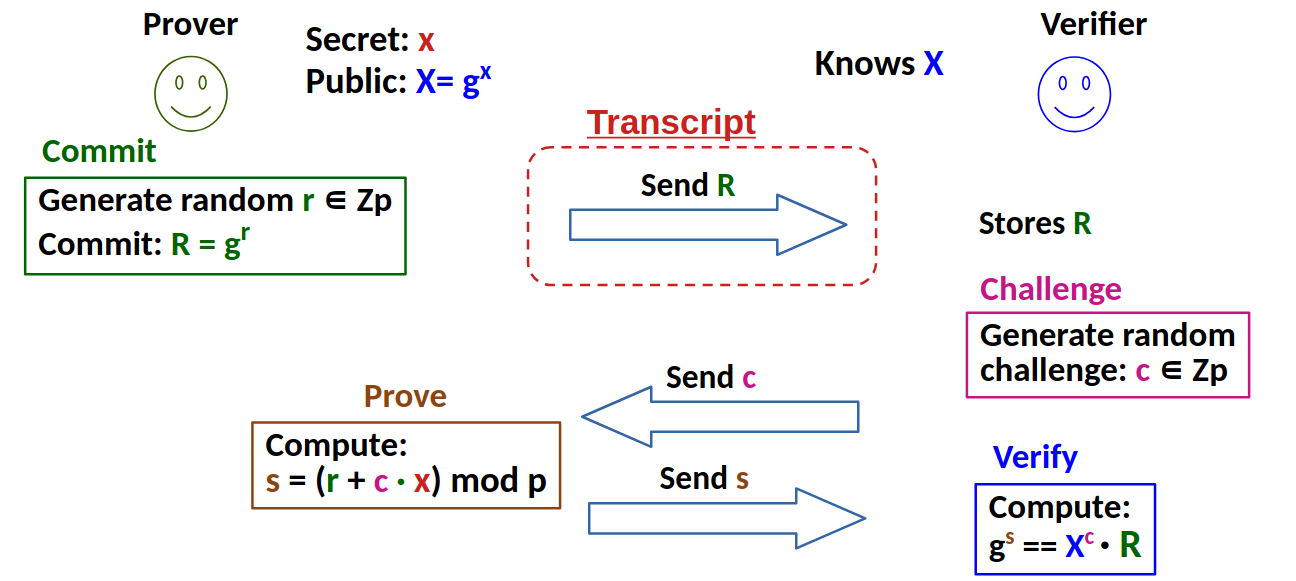
\includegraphics[width=0.95\textwidth]{img/schnorr_ip.png}
        \caption{\textit{Schnoor Signature}}
        \label{fig:schnorr_ip}
    \end{figure}

    \begin{figure}[h]
        \centering
        \begin{minipage}[c]{0.45\textwidth}
            \textbf{Note}: il \textbf{\textit{commitment}} vincola il \textit{prover} su un certo $r$ e non può cambiarlo dopo aver visto la \textit{challenge} $c$ (questo impedisce attacchi dell'\textbf{immagine iniziale}). Il \textit{verifier} sceglie la \textit{challenge} $c$ in maniera \textbf{casuale} questo impedisce al \textit{prover} di precostruire un $s$ e un $R$ in maniera malevola. Siccome $s = r + c \cdot x$ garantisce che $r$ non sia scelto a posteriori.
        \end{minipage}
        \hfill
        \begin{minipage}[c]{0.45\textwidth}
            \begin{align*}
                & \textcolor{olive}{\textbf{Dimostrazione}} \quad & \\
                g^s &\equiv_p X^c \cdot R \\
                g^{r + c \cdot x} &\equiv_p X^c \cdot R \\
                g^r \cdot g^{c \cdot x} &\equiv_p X^c \cdot R \\
                R \cdot X^c &\equiv_p X^c \cdot R
            \end{align*}
        \end{minipage}
    \end{figure}

    \medskip

    \textcolor{red}{\textbf{[3] \textit{Non-Interactive Zero-Knowledge proof of secret Exponent + Fiat-Shamir Heuristic (Transformation)}}}

    \begin{figure}[h]
        \centering
        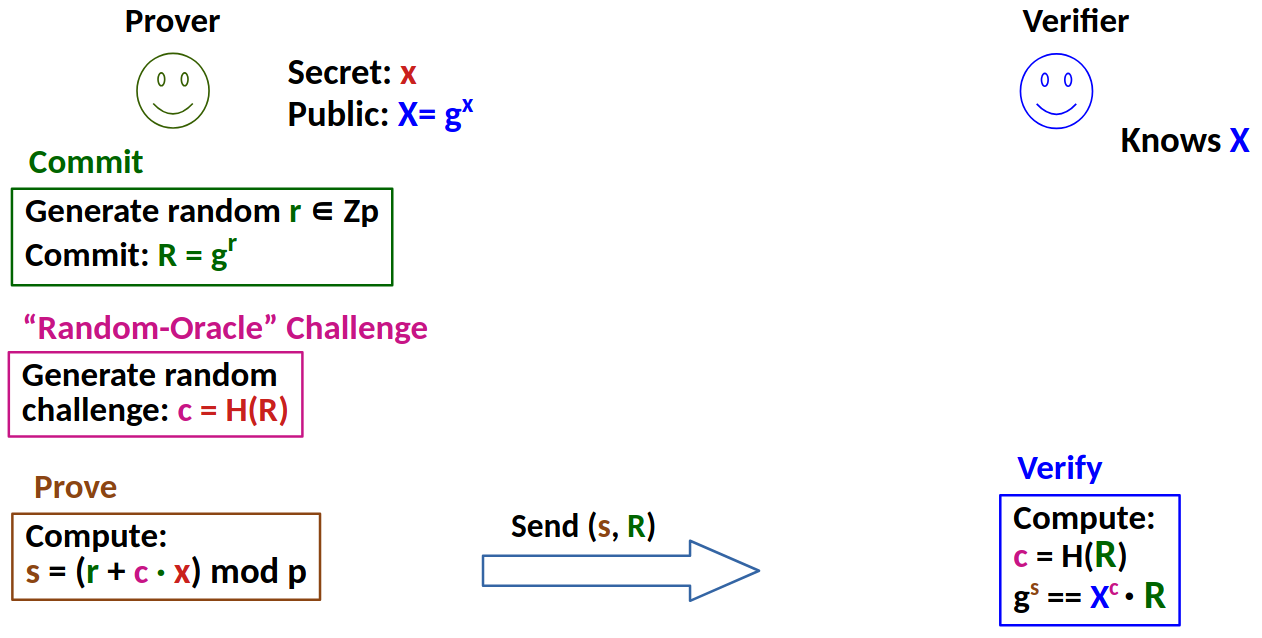
\includegraphics[width=0.95\textwidth]{img/fiat_shamir_ip.png}
        \caption{\textit{NIZKP}}
        \label{fig:fiat_shamir_ip}
    \end{figure}

    La \textit{Fiat-Shamir Heuristic} traduce qualunque \textbf{ZKP interativo} in un \textbf{NIZKP}, tuttavia aggiunge una congettura legata all'adozione di una funzione \textbf{\textit{random oracle challenge}}.
    \begin{itemize}[nosep]
        \item con \textbf{messaggi}: la \textbf{\textit{random challenge}} verrebbe calcolata $H(R \; || \; m)$ dove $m$ è il messaggio. Il \textit{prover} invierebbe al \textit{verifier} la tupla $(m, (s, R))$
        \item in alcuni casi è possibile \textbf{esplicitare la chiave pubblica} andando a calcolare la \textbf{\textit{random oracle challenge}} come $H(X \; || \; R \; || \; m)$ dove $X$ è appunta la chiave pubblica. Utili per contrastare alcuni casi di attacco in cui il \textit{verifier} venga indotto ad utilizzare un $X$ che è diverso da quello calcolato con $g^x \mod p$
    \end{itemize}

    Sono presenti anche delle varianti per quanto riguarda la \textbf{\textit{Schnorr signature}} (Fig.~\ref{fig:schnorr_ip}):

    {\centering
        \centering
        \begin{minipage}[t]{0.45\textwidth}
            \centering
            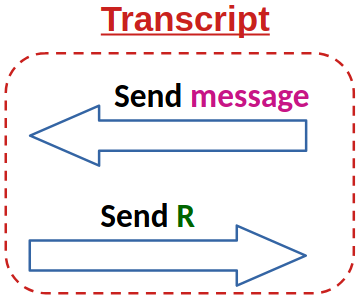
\includegraphics[width=0.55\textwidth]{img/schnorr_message_ip.png}

            \begin{flushleft}
                In questo caso il \textit{verifier} comunica un messaggio che il \textit{prover} dovrà firmare.
            \end{flushleft}

        \end{minipage}
        \hfill
        \begin{minipage}[t]{0.45\textwidth}
            \centering
            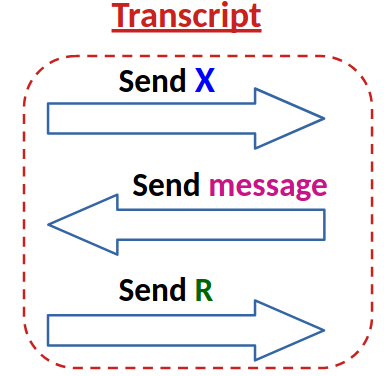
\includegraphics[width=0.55\textwidth]{img/schnorr_mX_ip.png}

            \begin{flushleft}
                In questo caso il \textit{prover} invierà prima la chiave pubblica utilizzate e successivamente il \textit{verifier} invierà il messaggio da firmare
            \end{flushleft}
        \end{minipage}
    \par}
    
    I protocolli considerati sono \textbf{probabilistici}, calcolano un random $r$ per il \textit{commitment} che - normalmente - non viene mai fornito nelle librerie. Se, però, $r$ è esposto o generato con una procedura sbagliata un avversario può ottenere la chiave segreta $x$.
    
    \smallskip

    \textcolor{red}{\textbf{\textit{Deterministic Variant}}}: generare il valore $r$ in modo \textbf{deterministico} a partire dal \textbf{messaggio} e dalla \textbf{\textit{secret key}} $x$, usando una \textbf{KDF}. Permette di evitare rischi critici dovuti alla riutilizzazione dell'$r$ e garantisce che la firma sia la stessa per uguali messaggi.
    In questo caso $r = \text{KDF}(x, m)$, la procedura per generare $r$ è \textbf{opaca} (non sa nulla) al \textit{verifier} anche perché $r$ è segreto e solamente $R$ gli viene inviato.

    \smallskip

    \textcolor{red}{\textbf{\textit{Hybrid Approaches}}} anche chiamato \textbf{\textit{hedged}} unisce la variante \textbf{deterministica} e se presente una sorgente di entropia, allora utilizza anche un valore randomico. In questo caso viene generato un $r_1 \in \mathbb{Z}_p$ e successivamente $r$ sarà calcolato come $r = \text{KDF}(x, \; \text{salt}=r_1, \; \text{info}=m)$

    \medskip

    \textcolor{red}{\textbf{\textit{EdDSA Signature (Ed22519)}}}

    \begin{figure}[h]
        \centering
        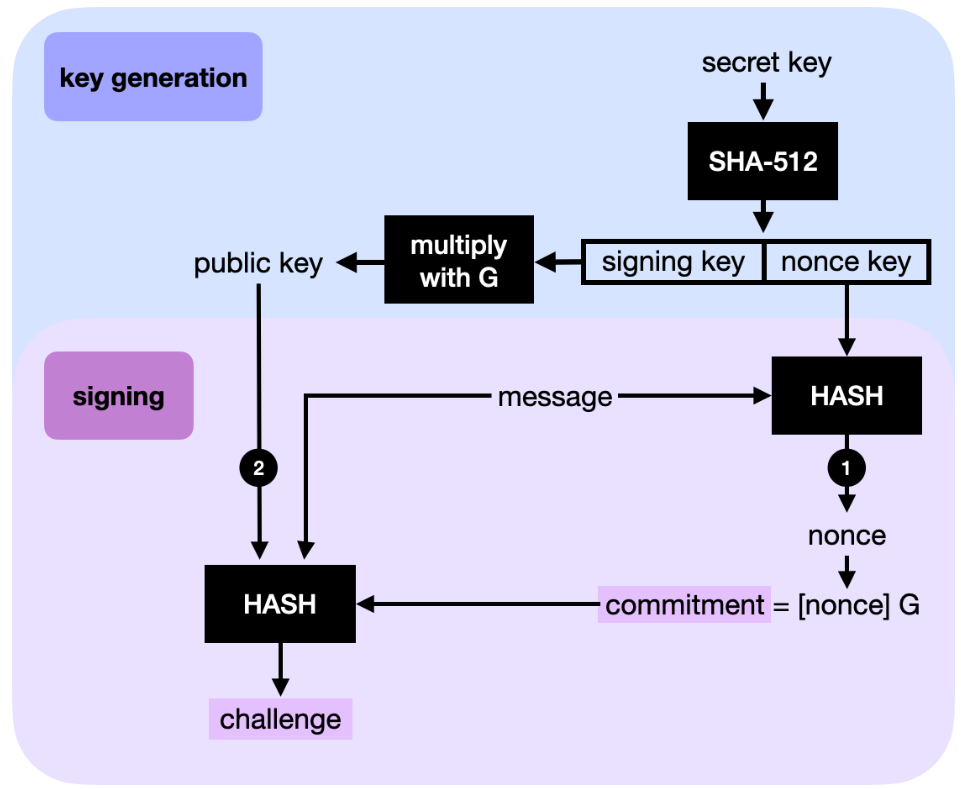
\includegraphics[width=0.75\textwidth]{img/eddsa.png}
    \end{figure}

    \textbf{SHA512} è la funzione che permette di avere chiavi \textbf{non correlate}, viene utilizzato un \textbf{HASH} per generare un ``\textbf{SIV}'' e l'altra come \textit{fiat-shamir-transformation}. \\
    Lo standard NIST per firma digitale su curve ellittiche è \textbf{ECDSA} e può essere considerata una variante della progettazione di Schnorr. \textcolor{red}{\textbf{(extra) Equazioni}}: vedi ``Algoritmi di Crittografia''.

\end{flushleft}

\begin{flushleft}
    \begin{figure}[h]
        \centering
        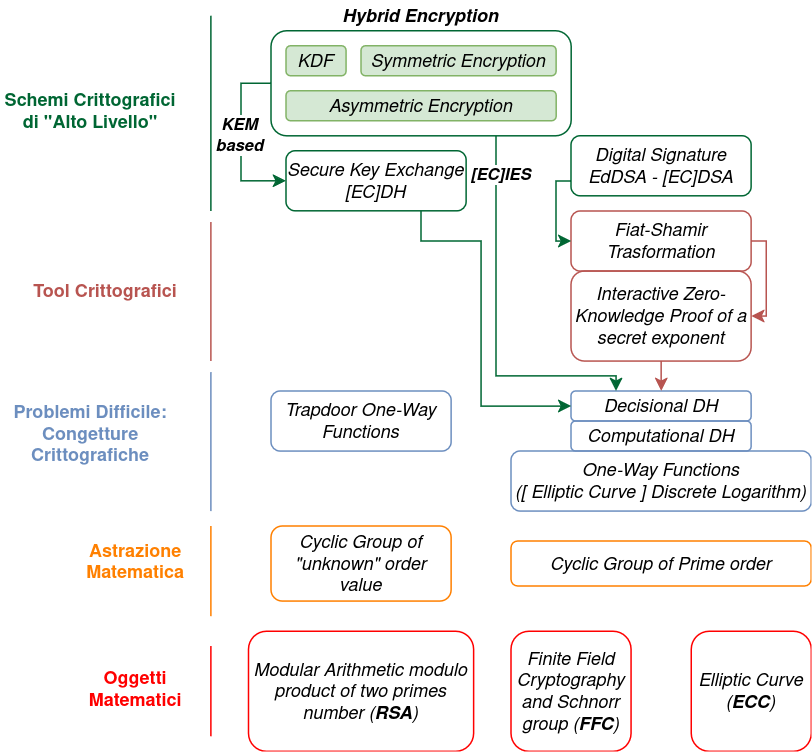
\includegraphics[width=\textwidth]{img/md_crypto_2.png}
        \caption{Mappa per gli schemi basati su \textit{[EC]DH}}
    \end{figure}
\end{flushleft}

\section{(extra) Cryptography Scheme based on RSA: PKCS\#1}
\section{(extra) "Asymmetric" Cryptography}

% PAGINA VUOTA
%\clearpage\null\thispagestyle{empty}\clearpage
%\appendix
%\appendixpage
%\addappheadtotoc

%\clearpage\null\thispagestyle{empty}\clearpage


%\listoffigures


\begin{flushleft}
\bibliographystyle{plain}
\bibliography{sections/references} 
\end{flushleft}

\end{document}
